%!inizio
\documentclass[twoside,openright]{report}
\usepackage{etoolbox}
\usepackage{emptypage}
\makeatletter
\let\LaTeXStandardPart\part%
\newcommand{\unstarredpart@@noopt}[1]{%
  \unstarredpart@@opt[#1]{#1}%
}%
\newcommand{\unstarredpart@@opt}[2][]{%
  \cleardoublepage% (For clearing content before!!!)
  \begingroup%
  \let\newpage\relax%
  \LaTeXStandardPart[#1]{#2}%
  \endgroup%
}%
\newcommand{\starredpart}[1]{%
  \LaTeXStandardPart*{#1}%
}%
\newcommand{\unstarredpart}{%
  \@ifnextchar[{\unstarredpart@@opt}{\unstarredpart@@noopt}%
}%
\renewcommand{\part}{%
  \@ifstar{\starredpart}{\unstarredpart}%
}%

\usepackage{helvet}
\usepackage[strict]{changepage}
\usepackage{lscape}

\usepackage{xcolor}
\definecolor{mybordeaux}{HTML}{AC3239}
\definecolor{myblu}{HTML}{0066cc}
\definecolor{myblack}{HTML}{000000}
\definecolor{mygreen}{HTML}{006600}

\usepackage{sectsty}
\chapterfont{\color{mybordeaux}}
\partfont{\color{mybordeaux}}
\usepackage{cleveref}
\usepackage{cite}


\usepackage[ ]{titlesec}
 
\titleformat{\chapter}[display]
{ \bf \huge \color{mybordeaux}}
{\flushright \normalsize \color{myblack} \MakeUppercase { \chaptertitlename } \hspace{1 ex} { \fontsize{60}{60}\selectfont \color{myblack} \sffamily  \thechapter }} {10 pt}{\huge}

\titleclass{\part}{top} % make part like a chapter
\titleformat{\part}
[display]
{ \raggedleft\normalfont\Huge\bfseries  \color{myblu}}
{\titlerule[0pt]\vspace{3pt}\titlerule[0pt]\vspace{3pt}\MakeUppercase{\partname} \thepart}
{0pt}
{\titlerule[0pt]\vspace{1pc}\huge\MakeUppercase}
%
\titlespacing*{\part}{0pt}{0pt}{20pt}


\usepackage{algorithm}
\usepackage{algorithmic}
\newsavebox{\ieeealgbox}
\newenvironment{boxedalgorithmic}
{\begin{lrbox}{\ieeealgbox}
\begin{minipage}{\dimexpr\columnwidth-2\fboxsep-2\fboxrule}
\begin{algorithmic}}
{\end{algorithmic}
\end{minipage}
\end{lrbox}\noindent\fbox{\usebox{\ieeealgbox}}}

\usepackage{subfig}
\usepackage{graphicx}
\graphicspath{{eps/}}
\DeclareGraphicsExtensions{.eps,.pdf,.jpeg,.png}
\usepackage[cmex10]{amsmath}

\usepackage[pagebackref, pdfstartview=Fit, bookmarksnumbered]{hyperref}
\hypersetup{  
       bookmarksopenlevel=2,
       bookmarksopen=true,
%       bookmarks=true,       % show bookmarks bar
%    unicode=false,          % non-Latin characters in Acrobat bookmarks
       pdftoolbar=false,        % show Acrobat toolbar?
       pdfmenubar=false,        % show Acrobat menu?
       %pdffitwindow=true,     % window fit to page when opened
       %pdfstartview={FitH},    % fits the width of the page to the window
       pdftitle={Resources Optimization for Distributed Mobile Platform in Smart Cities},    % title
       pdfauthor={Daniela Mazza},     % author
       pdfsubject={Urban Mobile Cloud Computing},   % subject of the document
       pdfcreator={Daniela Mazza},   % creator of the document
       pdfproducer={Producer}, % producer of the document
       pdfkeywords={Smart City, Resources Optimization, MCC, Computation Offloading, HetNets, Distributed Systems, 5G}, % list of keywords
    pdfnewwindow=true,      % links in new PDF window
    colorlinks=true,       % false: boxed links; true: colored links
    linkcolor=myblu,          % color of internal links (change box color with linkbordercolor)
    citecolor=mygreen,        % color of links to bibliography
    filecolor=myblack,      % color of file links
    urlcolor=myblu,           % color of external links
    pdfpagemode=UseOutlines,
    pdffitwindow=true
}

\usepackage{suthesis-2e}

\usepackage{enumitem}
\newcommand{\subscript}[2]{$#1 _ #2$}
\def\algorithmautorefname{Algorithm}



\usepackage[figuresright]{rotating}

\usepackage[acronym,shortcuts]{glossaries}
\setacronymstyle{long-short}
\makeglossaries

\input{vociglossario}
\dept{Electrical, Electronic and Information Engineering (DEI) Guglielmo Marconi}

\usepackage{fancyhdr}
\pagestyle{fancy}
%!hyphenation
\hyphenation{op-tical net-works semi-conduc-tor tech-nology infra-structure submitted}


\begin{document}



\title{Resources Optimization \\for Distributed Mobile Platforms \\in smart cities}
\author{Daniela Mazza Candidate}
\principaladviser{Prof. Giovanni Emanuele Corazza}
\firstreader{Prof. Daniele Tarchi}
\secondreader{Prof. Mohsen Guizani}
\thirdreader{Prof. Flavio Bonomi} %if needed
%\fourthreader{Severus Snape} %if needed

%!frontespizio
\hypersetup{pageanchor=false}
\begin{titlepage}
\begin{adjustwidth}{-4em}{-1cm}
\center
\vspace*{-2cm}
{\LARGE{\textsf{\textbf{ALMA MATER STUDIORUM  --\ UNIVERSITA' DI BOLOGNA}}}}

\vspace*{2cm}
{\LARGE{\textsf{DOTTORATO DI RICERCA IN}}}

\vspace{0.5cm}
\LARGE{\textsf{Elettronica, Telecomunicazioni \\ e Tecnologie dell'Informazione}}

\vspace{0.5cm}
{\LARGE{\textsf{Ciclo XXVIII}}}
\vspace{0.8cm}
\flushleft        
{\Large{\textsf{\textbf{Settore Concorsuale di afferenza:} 09/F2}}}  

\vspace{0.8cm}
{\Large{\textsf{\textbf{Settore Scientifico Disciplinare:} ING-INF/03}}}   
\vspace{0.8cm}
\center
\vspace{0.8cm}
{\LARGE{\textsf{RESOURCES OPTIMIZATION \\
FOR DISTRIBUTED MOBILE PLATFORMS \\ IN SMART CITIES}}}

\vspace{0.5cm}   
\flushleft
%{\Large{\textsf{\textbf{Presentata da:} Daniela Mazza\\}}}  


\begin{minipage}[t]{0.5\textwidth}
{\Large{\textsf{\textbf{Presentata da:} Daniela Mazza\\}}}  \\
{\Large{\textsf{\textbf{Coordinatore Dottorato:}}}}\\
{\Large{\textsf{Prof. Alessandro Vanelli Coralli}}}
\end{minipage}
\hfill
\hfill
\hfill\hfill\hfill\hfill\hfill\hfill
\begin{minipage}[t]{0.5\textwidth}
{\Large{\textsf{\textbf{Relatore:}}}}\\
{\Large{\textsf{Prof. Giovanni Emanuele Corazza}}}\\
{\Large{\textsf{\textbf{Correlatore:}}}}\\
{\Large{\textsf{Prof. Daniele Tarchi}}}
\end{minipage}

\vspace{1cm}
\center
{\Large{\textsf{\textbf{Esame finale anno 2016}}}}
\end{adjustwidth}
\end{titlepage}
\hypersetup{pageanchor=true}
\cleardoublepage

\beforepreface
%!dedica
\chapter*{}
\begin{flushright} 
\textit{To my family} 
\end{flushright}

\bigbreak
\bigbreak
\bigbreak
\bigbreak
\bigbreak
\bigbreak
\bigbreak
\bigbreak
\bigbreak
\bigbreak
\bigbreak
\bigbreak
\bigbreak
\bigbreak
\bigbreak
\bigbreak
\bigbreak
\bigbreak
\bigbreak
\bigbreak

''I am struck by how, except when you're young, you really need to prioritize in life, figuring out in what order you should divide up your time and energy. If you don't get that sort of system set by a certain age, you'll lack focus and your life will be out of balance.''
\bigbreak

\hfill Haruki Murakami, \textit{What I Talk About When I Talk About Running}
%\chapter*{}

%!Abstract
\prefacesection{Abstract}
This thesis collects the outcomes of a Ph.D. course in Electronics, Telecommunications, and Information Technologies Engineering and it is focused on the study and design of techniques able to optimize resources in distributed mobile platforms. It is related to a typical \emph{smart city} environment, in order to enhance quality, performance and interactivity of urban services. 
The subject is the operation of \emph{computation offloading}, intended as the delegation of certain computing tasks to an external platform, such as a cloud or a cluster of devices.
Offloading the computation tasks can effectively expand the usability of mobile devices beyond their physical limits and may be necessary due to limitations of a  system handling a particular task on its own. 

The computation offloading within an ecosystem as a urban community, where a large amount of users are connected towards even multiple devices, is a challenging subject. 
In a very close future, smart cities will be  peculiar sources of intensive computing tasks, since they are conceived as systems where e-governance will be not only transparent and fast, but also oriented to energy and water conservation, efficient waste disposal, city automation, seamless facilities to travel and affordable access to health management systems. 
Also traffic will need to be monitored intelligently, emergencies foreseen and resolved quickly, homes and citizens provided with a wide series of control and security devices.
All these ambitious aspirations will require the deployment of infrastructures and systems where devices will generate massive data and should be orchestrated in a collective way, to pursue synergic goals. 
In this context, the computation offloading is an operation dealing with the optimization of urban services, in order to reduce costs and consumption of resources and to improve the connection between citizens and government. 

This dissertation is organized in three main parts, dealing with the optimization of the resources in a smart city background from different points of view.

The first part introduces the \gls{UMCC} framework,  a system model that takes into account a series of features related to \glspl{HetNet}, cloud architectures, various characteristics of the \glspl{SMD} and  different types of smart city application, performed to pursue several goals. 

The second part deals with a partial offloading operation, taking into account the possibility of delegating towards a cloud infrastructure only a portion of the computation load. It is focused on the tradeoff between energy consumption and execution time, in a non-trivial multi-objective optimization approach. Furthermore, a utility function model developed from the economic field is introduced, in order to optimize the system. It  takes into account a series of parameters related to the \gls{UMCC}, showing that, when the network is overloaded, the partial offloading operation allows to achieve the target throughput values although the energy consumption and the computational time consumed in the partial offloading are lower than the resources consumed in the total offloading operation. 
In addition, the proposed \gls{UMCC} framework and the partial computation offloading are applied to a vehicular environment for handling a real-time navigation application, so that the \glspl{SMD} can exploit road side units and other neighbor devices forming clusters for delegating a shared application. It is shown that the clusterization allows to reduce the consumed energy in case of high traffic scenarios, optimizing the cluster size for different populations size and various offloading policies.

Finally, in the third part, the problem of \gls{CA} in a \gls{UMCC} framework deals with the system as a community, thinking about improving the collective performance and not only the achievement of a single device.
A probabilistic algorithm that uses biased-randomization techniques is proposed as an efficient alternative to exact methods, which require unacceptable levels of computational time to solve real life instances. 
This probabilistic algorithm is able to provide near-optimal solutions in real time, thus outperforming by far the solutions provided by existing greedy heuristics. 
Since this algorithm takes into account all users in the assignment process, it avoids the selfish or myopic behavior of the greedy heuristic and, at the same time, is able to quickly find near-optimal solutions for the allocation of the available resources.



\prefacesection{Introduction}
%!Introduction
According to the flagship publication of the United Nations \emph{World Urbanization Prospect}\footnote{\url{http://esa.un.org/unpd/wup/}}, more than one half of the world population is living nowadays in urban areas, and about 70\% will be city dwellers by 2050. 
Furthermore, the world population is estimated to increase in the second half of the 21\textsuperscript{st} century, while the urban areas are expected to absorb all the predicted growth and to draw in some of the rural population. 
The United Nations report predicts that,  by mid-century, there will be 27 \emph{megacities}, with at least 10 million population, while at least half of the urban growth in the coming decades will occur in small cities with less than 500,000 people, envisioning therefore that cities, big or small, are becoming a determining shift in the organization of human society. 
Cities and megacities are predicted to magnify problems such as difficulty in waste management, scarcity of resources, air pollution, human health concerns, traffic congestion, and inadequate, deteriorating and aging infrastructures.

Concurrently with such urbanization effect, an extraordinary phenomenon concerning the \gls{ICT} is happening: smart mobile devices are becoming an essential part of human life and the most effective and convenient communication tools, not bounded in time and place.
According to the Cisco \emph{Visual Networking Index}\footnote{\url{http://www.cisco.com/c/en/us/solutions/service-provider/visual-networking-index-vni/index.html}}, the number of mobile-connected devices has already overtaken the number of people in the world, and by 2018 it will be over 10 billion, including \gls{M2M} modules. 
Overall mobile data traffic is expected to have nearly an 11-fold increase in the next five years. 

Urbanization tendency and smart mobile expansion are going to reach a relevant convergence point through the concept of smart city, an icon of a sustainable and livable city, projecting the ubiquitous and pervasive computing paradigms to urban spaces, focusing on developing city network infrastructures, optimizing traffic and transportation flows, lowering energy consumption and offering innovative services. 
It is through \gls{ICT} that smart cities are truly turning \emph{smart}~\cite{Ratti}, in particular by means of the exploitation of smart mobile devices, forming together with cloud computing the \gls{MCC}, since, as suggested by Michael Batty, \textit{to understand cities we must view them not simply as places in space but as systems of networks and flows}~\cite{Batty}. 

In this context a new urban framework, named \gls{UMCC}, is introduced in this thesis.  It can be thought as the technological nervous system allowing the networks and flows of the city for achieving a better urban way of life. 
By means of the \gls{UMCC} framework, and considering various configurations of clouds and networks, data storage and processing can be dynamically delegated to resource-rich devices, thus shortening execution time, extending battery life and exploiting the possibility to preserve data in the cloud.

The \gls{UMCC} framework can effectively support a smart city \emph{vision}, gathering, collecting and processing data in real time, aiming to take advantage of the most advanced communication technologies, to hold up added-value services for the administration of the city and for the citizens. 
The resources optimization, within the \gls{UMCC} framework, can be driven by purposely defined cost functions, including throughput, energy efficiency, latency and computing performance. 
The challenges and the exploiting opportunities of  the \gls{UMCC} are discussed in relation to smart city solutions, highlighting the features that can affect the \gls{QoS} of various types of smart city related applications.
%!Original Contributions
\prefacesection{Original Contributions}
In this dissertation, innovative techniques and methodologies aimed to enhance the performance of \gls{MCC} applied to a smart city are proposed and investigated.
In particular the \gls{UMCC}, a global framework that can be adapted depending on the optimization objectives is introduced, highlighting the features that can affect the \gls{QoS} of various types of smart city-related applications.
Furthermore, various optimization techniques, based on opportunely defined cost or utility functions, are presented and inspected for the optimization of the resources in the \gls{UMCC}.
Specifically:
\begin{itemize}
\item a partial offloading tecnique is determined for optimizing time and energy consumption in a smart city \glspl{HetNet} scenario, where smart mobile devices are supposed to perform a distributed application;
\item
a utility function model derived from the economic world has been presented, aiming to measure the \gls{QoS}, in order to choose the best access point in a \gls{HetNet} for offloading part of an application on the \gls{MCC};
\item 
a cluster-based optimization technique is proposed and utilized in a distributed computing resource allocation, exploiting resource sharing, in high density \gls{SMD} environments.
\end{itemize}

During my Ph.D. course I had the opportunity to collaborate with the Internet Interdisciplinary Institute (IN3) at the Open University of Catalonia (UOC), where I contributed to  develop new optimization heuristics for improving heterogeneous communication systems. 
The applied approach is based on the use of biased randomization techniques, which have been used in the past to solve similar combinatorial optimization problems in the fields of logistics, transportation, and production. 
This work extends the use of these biased randomization techniques to the field of smart cities and mobile telecommunications. 
Some numerical experiments contribute to the validation of the proposed approach.

The outcomes of this research stay are described in \autoref{chap:socialBRA}. 

\section*{Personal Publications}
\begin{enumerate}[label={[}\subscript{P}{\arabic*}{]}]
 \item \label{P1}
   D. Mazza, D. Tarchi, and G. Corazza, {"}A Unified Urban Mobile Cloud Computing Offloading Mechanism for Smart Cities{"} \textit{Communications Magazine, IEEE, Feb. 2016 (SUBMITTED)}
    \item \label{P2}
    D. Mazza, A. Pages, D. Tarchi, A. Juan, and G. E. Corazza, {"}A biased-randomized algorithm for mobile cloud computing in smart cities,{"} \textit{Systems Journal, IEEE, Oct. 2015 (SUBMITTED)}
\item \label{P3}
D. Mazza, D. Tarchi, and G. Corazza, {"}A cluster based computation offloading technique for mobile cloud computing in a smart city scenario,{"} \textit{in Proc. of IEEE Conference on Communication (ICC) 2016, Kuala Lumpur, Malaysia (ACCEPTED).}
\item \label{P4}
D. Mazza, D. Tarchi, and G. E. Corazza,  {"}A user-satisfaction based offloading technique for smart city applications,{"}  \textit{in Proc. of IEEE Globecom 2014, Austin, TX, USA, Dec. 2014.}
\item \label{P5}
D. Mazza, D. Tarchi, and G. E. Corazza,  {"}A partial offloading technique for wireless mobile cloud computing in smart cities, {"} \textit{in Proc. of 2014 European Conference on Networks and Communications (EuCNC), Bologna, Italy, Jun. 2014.}
%\item \label{P6}
%G. Avanzolini, A. Cappello, and D. Mazza, {"}Comparative evaluation of three elastance-resistance models of left ventricular mechanics,{"}  \textit{in Computers in Cardiology, in Proceedings., Sep. 1991, pp. 653-656.} 
\end{enumerate}

%!Acknowledgments
\prefacesection{Acknowledgments}
This Ph.D. dissertation was carried out during three years of my life in which not only I have gained knowledge and accomplished an academic path, but also I had the opportunity to proof and enrich my personality.
I would like to thank Prof.~Giovanni Emanuele Corazza  and Prof.~Daniele Tarchi for their precious advice and support during my Ph.D. studies. They helped me during every step of my work with unmatched competence and patience. 

A sincere thanks goes to Prof.~\'Angel Alejandro Juan P\'erez and Prof.~Adela Pag\'es Bernaus for giving me the chance to work with them at the DPCS IN3 Lab of the Open University of Catalonia: for their collaboration and for being always available to share projects and ideas and because my stay in Barcelona has been a unique experience for me, both professionally and personally. 

I am also deeply grateful to Prof.~Alessandro Vanelli Coralli, Coordinator of the Ph.D. Program in Electronics, Telecommunications, and Information Technologies, for making it possible to carry out this work. 
 
A special acknowledgment goes also to all my colleagues that shared with me many important moments during my time at the University of Bologna - Roberta, Sergio, Vahid, Vincenzo - and at the Internet Interdisciplinary Institute IN3 in Barcelona - Aljoscha, Carlos, Jesica, Laura, Helena.

I also want to thank the reviewers of this thesis, Prof. Flavio Bonomi and Prof. Mohsen Guizani, for their many suggestions and help for greatly improving the quality of this work.

Infine, il pi\'u grande ringraziamento va alla mia famiglia. Grazie a Gabriele, mio compagno di vita, per aver condiviso la mia esperienza e per avermi supportato e incoraggiato, ai miei genitori, per avermi infuso l'amore per lo studio, e a mio figlio Alessandro, che sempre mi ha dato la forza per continuare a dedicarmi alla ricerca.
\afterpreface
\part{Urban Mobile Cloud Computing: a framework at the service of smart cities}
Innovative designs of smart cities, aiming at realizing a vision where municipalities can use information and communications technologies to meet sustainability goals, boost local economies, and improve urban services, have been and are being adopted in the political agenda of many governments as a primary program, in a large number of developed and developing countries. This development is in line with the evolutionary trends in the Information Society \cite{technologyAsANeed2010}.

The ever-growing demand for services from citizens and institutions, intending to make the cities \textit{smarter} and improve the quality of life of the communities, has given a great boost to the conception of diverse wireless communication systems and has extended the envision of cloud architectures for providing infrastructures (\gls{IaaS}), platforms (\gls{PaaS}), and software (\gls{SaaS})\cite{CCTaxonomy,fantacci09} , offering computation, storage and network and going towards the integration with novel opportunistic communications as fog networking~\cite{opportunistic, Bonomi2012, Bonomi2014}.

In order to  interact with city services, \gls{MCC} and wireless \glspl{HetNet} contribute in different and sinergic way for handling this smart city scenario, allowing ubiquitous and pervasive computing in a framework we called \gls{UMCC}.

In this first part of the dissertation, the proposed \gls{UMCC} system model is described and investigated. It takes into account a series of features related to \gls{HetNet}'s nodes, cloud architectures, \glspl{SMD}' characteristics, in association with several types of application and goals - mobility, healthcare, energy and waste management, and so on. 
It can be employed in the optimization of the \gls{QoS}'s requirements related to the needs of citizens. 

Smart cities applications are gaining an increasing interest among administrations, citizens and technologists for their suitability in managing the everyday life. 
One of the major challenges is managing in an efficient way the presence of multiple applications in this \gls{UMCC} framework, in a Wireless \gls{HetNet} environment, alongside the presence of a \gls{MCC} infrastructure. 

\vspace{1cm}
\textit{The content of the following chapter was extracted from publications \hyperref[P1]{[P1]}, \hyperref[P2]{[P2]}, \hyperref[P3]{[P3]} and \hyperref[P4]{[P4]}}

\chapter[The UMCC architecture]{The Urban Mobile Cloud Computing Architecture}
\label{chap:UMCC}
\section{Introduction to the UMCC in a smart city scenario}
The increasing urbanization level of the world population has driven the development of technology toward the definition of a smart city geographic system, conceived as a wide area characterized by the presence of a multitude of smart devices, sensors and processing nodes aiming to distribute intelligence into the city; moreover, the pervasiveness of wireless technologies has led to the presence of heterogeneous networks operating simultaneously in the same city area. 
One of the main challenges in this context is to provide solutions able to optimize jointly the activities of data transfer, exploiting the heterogeneous networks, and data  processing, by using different types of devices. 
In this chapter, the \gls{UMCC} framework is introduced, considering a mobile cloud computing model that describes the flows of data and operations taking place in the smart city scenario. 

The challenges and the opportunities of exploiting the \gls{UMCC} are discussed in relation to smart city solutions, highlighting the features that can affect the \gls{QoS} of various types of smart city-related services.

The  \gls{UMCC} sprang from the \gls{MCC}, that is gaining an increasing interest in the recent years, due to the possibility of exploiting both cloud computing and mobile devices for enabling a distributed cloud infrastructure~\cite{DinhSurvey}. 
Considering the peculiarity of the  \gls{MCC}, we can observe that, on one hand, the cloud computing idea has been introduced as an enabling technology for allowing remote computation, storage and management of information, and, on the other hand, the mobility skill allows to gain by the most modern smart devices and broadband connections for creating a distributed and flexible virtual environment. 
At the same time, the recent advances in the wireless technologies are defining a novel pervasive scenario where several heterogeneous wireless networks interact among them, giving users the ability to select the best network choosing among those present in a certain area.
As a consequence, the development of the \gls{UMCC} is introduced, gaining from both computing and wireless communication technologies. It is a challenging opportunity for the creation of smart city infrastructures, providing solutions fulfilling the urgent need for richer application and services, requested from citizens that, as mobile users, are facing many demanding tasks in relation to mobile device resources as battery life, storage and bandwidth. 
\subsection*{The triple role of Smart Mobile Devices}
By analyzing the technology systems underlying a smart city framework, mobile devices can be considered in a three-fold way, as illustrated in \autoref{fig:SMDclassification}:
\begin{itemize}
\item \textbf{Sensors:} They can acquire different types of data regarding the users and the environment, transmitting a large amount of information to the cloud in real time, by means of wireless communication systems. 
This is the underlying concept leading to the \gls{IoT} network, profitably exploited to improve urban life, for instance for extracting descriptive and predictive models in the urban context of cities~\cite{IoTCC}. As well as the expansion of Internet-connected automation into a plethora of new application areas, \gls{IoT} is also expected to generate large amounts of data from diverse locations, with the consequent necessity for quick aggregation of the data, and an increase in the need to index, store, and process such data more effectively. 
\item \textbf{Nodes:} They can form distributed mobile clouds where the neighboring mobile devices are merged for resource sharing, becoming integral part of the network. 
Furthermore, they can form \glspl{VCN} offering content routing, security, privacy, monitoring, virtualization services~\cite{Gerla}, easy to be used for providing smart city services and applications, in particular for traffic and mobility control. 
This is the crucial concept of fog networking, where a collaborative multitude of users carry out a substantial amount of storage, communication, and data management in a collaborative way.
\item \textbf{Outputs:} They can make the citizens aware of results and able to decide consequently, or become actuators without need of human intervention. This is the concept underlying \gls{M2M} communications where computers, embedded processors, smart sensors, actuators and mobile devices acquire information and act in an autonomous way~\cite{M2M}.
\end{itemize}
To perform this triple role, mobile devices have to become part of an infrastructure that is constituted by different cloud topologies and, at the same time, have to exploit heterogeneous wireless link technologies, allowing to address the different requirements of a smart city scenario. This infrastructure starts from the concept of \gls{MCC}, where the cloud works as a powerful complement to resource-constrained mobile devices.

\begin{figure}[tbp]
\centering
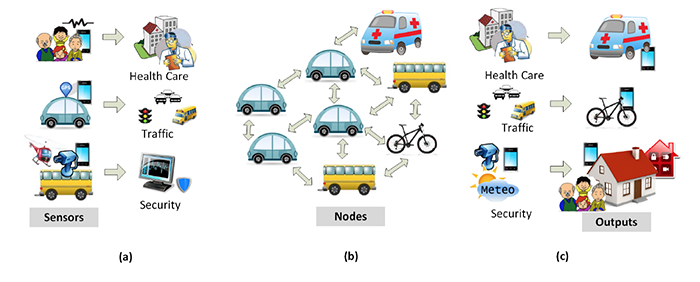
\includegraphics[width=\columnwidth]{SMDclassification}
\caption{Mobile devices acting in the UMCC framework as (a) sensors, (b) nodes, (c) outputs.}
\label{fig:SMDclassification}
\end{figure}

The vision of \gls{MCC} has increasingly become a source of interest, beginning from the early 2000s, when Amazon realized that a huge amount of space on their premises was underused. 
This awareness pushed toward the implementation of remote services, gaining by the presence of storage space and computing power and creating a cloud system. 
Alongside with the expansion of wireless technologies, the cloud computing has been integrated through a broadband system, exploiting the opportunity of working in mobility. 
The \glspl{SMD}, then, can use \gls{MCC} devolving demanding tasks and referring to it for data storage.  
\subsection*{Computation Offloading} 
The strategy allowing to delegate to one or more cloud computing elements storage and computing functions is commonly called \emph{cyberforaging} or \emph{computation offloading}. It allows to tackle with the limited battery power and computation capacity of the \glspl{SMD}, and plays a key role in a smart environment where wireless communication is of utmost relevance, particularly in mobility and traffic control domains~\cite{Barbarossa2014}.
If the storage is one of the most common and legacy activities that can be delegated to a remote cloud infrastructure, recently, thanks to modern programming paradigms, it is possible to allot even only a part of the computation load to a remote unit. 
This allows users to optimize the system performance by offloading only a fraction of the application to be computed, or distributing the application among different cloud structures. 
Offloading is an effective network congestion reduction strategy to solve the overload issue compared to scaling and optimisation \cite{Juniper}. It enables network operators to reduce the congestion in the cellular networks, while for the end-user it provides cost savings on data services and higher bandwidth availability.   

%Despite the combined advantages of cloud computing with the ubiquitous accessibility of mobile devices, the full potential of \gls{MCC} is far from being fully exploited. For instance, the primary role of mobile devices today in the context of cloud computing is to serve as terminals for accessing the cloud. If we look at the interaction pattern between the cloud and the mobile device today, an application can be either executed on the cloud side and use the mobile side as a thin client, or executed on the mobile side alone, while potentially consuming isolated cloud services such as map services in GPS-based applications. Even so, what can be executed on the cloud depends on what concrete services are provided by the cloud. This status quo limits the possibility and flexibility to optimize the mobile application performance [3].
%In a context of urban organization, such integrated \gls{UMCC} structure can be considered as the system that coordinates every function and action of a smart city.  
\section{Cloud Topologies}
\label{sec:CloudTopologies}
In relation to the \gls{SMD}'s roles previously described, we take into account various cloud topologies. This is a different categorization with respect to the common taxonomy used for cloud computing - \gls{SaaS}, \gls{PaaS} and \gls{IaaS}. It looks on the different interaction among the  nodes constituting the cloud, instead of the services provided by the cloud itself, so we can distinguish among centralized cloud, cloudlet, distributed mobile cloud and a combination of all, as shown in \autoref{fig:UMCC_topologies}. 
\subsection*{Centralized Cloud} 
A centralized cloud provides the citizens to interact remotely, e.g., for accessing to open data delivered by the public administrations. 
It refers to the presence of a remote cloud computing infrastructure having a huge amount of storage space and computing power, virtually infinite, offering the major advantage of the elasticity of resource provisioning. 
The centralized cloud infrastructure is often used for delivering the computing processes to remote clusters, owing a higher computing power, and/or for storing big amount of data. 
The centralized cloud allows to reduce the computing time by exploiting powerful processing units, but it could suffer from the distribution latency, due to the data transfer from the users to the cloud and \textit{vice versa}, the congestion, due to the multiple users exploitations, and the resiliency, due to the presence of a single performing infrastructure leading to the \gls{SPOF} issue.

\subsection*{Cloudlet}
One of the main drawback of the centralized cloud is the great distance between the mobile devices, requesting services, and the clusters, performing computation in the cloud. 
Even if the  \gls{SPOF} issue is often resolved by implementing mirroring or redundancy solutions, the big distance that may occur between users and centralized clouds can be better addressed by means of the introduction of cloudlets, representing small clouds installed in proximity of the users. 
Furthermore, the inclusion of cloudlets allows a most appropriate sizing depending on the number of contemporary requests of the users. 

Cloudlets are fixed small cloud infrastructures installed between the mobile devices and the centralized cloud, limiting their exploitation to the users in a specific area. 
Their introduction allows to decrease the latency of the access to cloud services by reducing the transfer distance at the cost of using smaller and less powerful cloud devices.

\subsection*{Distributed Mobile Cloud}
A third configuration can address the issue of non persistent connectivity, whereas both the previous concepts must assume a durable state of connection.  
In a distributed mobile cloud the neighboring mobile devices are pooled together for resource sharing~\cite{Fangming}.
An application from a mobile device can be either processed in a distributed and collaborative fashion on all the mobile devices or handled by a particular mobile device that acts as a server.

The possibility of implementing a distributed mobile cloud infrastructure has become a reality since the introduction of smarter and powerful mobile devices, e.g., smartphones, tablet, phablet, having the ability, even if limited, of computing and storaging. 
Moreover, it has to be noted that their number is still increasing, leading to a pervasive presence and allowing to form a \emph{cloud} of pervasive distributed devices that can interact among them.
This \emph{fog network} architecture uses one or a collaborative multitude of end-user clients or near-user edge devices to carry out a substantial amount of storage (rather than stored in centralized clouds), communication, and control, configuration, measurement and management \cite{Bonomi2012, Bonomi2014}.
It can be seen as the \emph{fog layer} that encapsulates phisical objects - equipped with computing, storage, networking, sensing, and/or actuating resources - and constitutes a piece of a wider \gls{CARS} architecture \cite{Guizani2014}, a geographically distributed platform that connects many billions of sensors and things, and provides multitier layers of abstraction of sensors and sensor networks, enabling the \gls{SenaaS}. 

 \subsection*{Combination of different topologies}
The proposed framework foresees the joint exploitation of the three aforementioned topologies. 
As outlined before, they are characterized by different features, leading to a different usage depending on the scenario. 
Hence, a joint exploitation could steer to a more efficient usage aiming to achieve the performance goals of a certain application.
As it will be better specified below, a smart city scenario is characterized by the presence of a lot of different applications, each one with different characteristics and requirements.
An integrated \gls{UMCC} framework composed by centralized clouds, cloudlets and distributed mobile clouds, as shown in \autoref{fig:UMCC_topologies}, allows to respect the application requirements with regard to other solution in a more efficient way.


\begin{figure}[tbp]
\centering
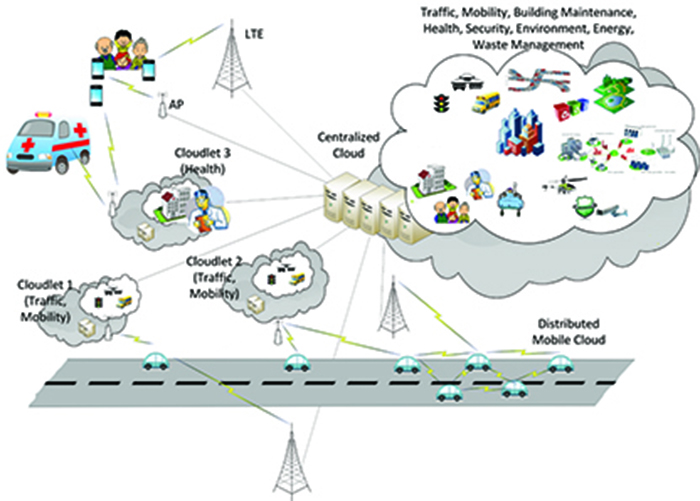
\includegraphics[width=\columnwidth]{UMCC_topologies}
\caption{Cloud topologies in the UMCC framework: centralized cloud, cloudlet and distributed mobile cloud.}
\label{fig:UMCC_topologies}
\end{figure} 





\section{Types of RATs}
\label{sec:TypesRATs}

In order to connect the devices, different types of \glspl{RAT} should be taken into consideration, providing a pervasive wireless coverage.

Multiple \glspl{RAT}, such as \gls{IEEE 802.11}, mobile \gls{WiMAX}, 
\gls{HSPA+}, \gls{LTE} and \gls{WiFi}, must be integrated to form a \gls{HetNet}. For enhancing the network capacity, generally there is an increasing interest in deploying relays, distributed antennas and small cellular base stations - \glspl{picocell}, \glspl{femtocell}, etc - indoors in residential homes and offices as well as outdoors in amusement parks and busy intersections. 
These new network deployments, comprised of a mix of low-power nodes underlying the conventional homogeneous macrocell network, by deploying additional small cells within the local-area range and bringing the network closer to users, can significantly boost the overall network capacity through a better spatial resource reuse. Inspired by the attractive features and potential advantages of \glspl{HetNet}, their development have gained much momentum in the wireless industry and research communities during the past few years. 
The heterogeneous elements are distinguished by their transmit powers/coverage areas, physical size, backhaul, and propagation characteristics. 

We can basically distinguish between two components, i.e., macrocells and small cells, where the former provide mobility while the latter boost coverage and capacity.

\subsection*{Macrocells}
The distance between the access points (base stations of the macrocells) is usually higher than 500~m. Thanks to this type of base stations the environment is completely covered and the devices can move by minimizing the handover frequency. On the other hand, in macrocells the system suffers for channel fading and traffic congestion. This leads to a lack of stability, not allowing to reach very high data rate. The technology used for this type of cells refers to the cellular networks, e.g. \gls{3G} and \gls{LTE}.
\subsection*{Small Cells} 
Small cells are characterized by low power radio access nodes, which have a cover range of about 100-200~m or less. We can distinguish between \glspl{picocell}, for providing hotspot coverage in public places - malls, airports and stadiums - without limits in terms of number of connected devices, and \glspl{femtocell}, for covering a home or small business area, available only for selected devices. \Glspl{picocell} and \glspl{femtocell} have been recently introduced as a way for increasing the coverage and maximize the resource allocation in \gls{LTE} networks. We also consider \gls{WiFi} access points as nodes with a small cover range (less than 100 m) which can typically communicate with a small number of client devices. However, the actual range of communication can vary significantly, depending on such variables as indoor or outdoor placement, the current weather, operating radio frequency, and the power output of devices.

 
\section{Challenges of the UMCC}
\label{sec:challenges}
The \gls{UMCC} approach foresees the definition of a scenario where smart city applications can exploit jointly the three topologies, as shown in \autoref{fig:offloading-distribution}, by distributing and performing among the different parts composing the framework. 
The application requested by a particular \gls{SMD}, signed as the \gls{RSMD}, is partitioned and distributed among the different clouds using the available \glspl{RAT}. In the example of \autoref{fig:offloading-distribution},  the application is divided among the centralized cloud, two cloudlets, and a distributed cloud formed by five devices. Furthermore, part of the application can be computed locally by the \gls{RSMD} itself.



The main issue is that, for transferring data from the requesting mobile device to the selected cloud topology, a certain time is required. 
This mostly depends on some communication parameters of the selected \gls{RAT}, such as the end-to-end throughput, the amount of users, the \gls{QoS} management of a certain transmission technology between the user device and each type of cloud processing unit. 
Furthermore, in terms of energy consumption, it should be taken into account the tradeoff between the energy saved in offloading part of the application to the cloud and the energy spent in sending the data. 

\begin{figure}[tbp]
\centering
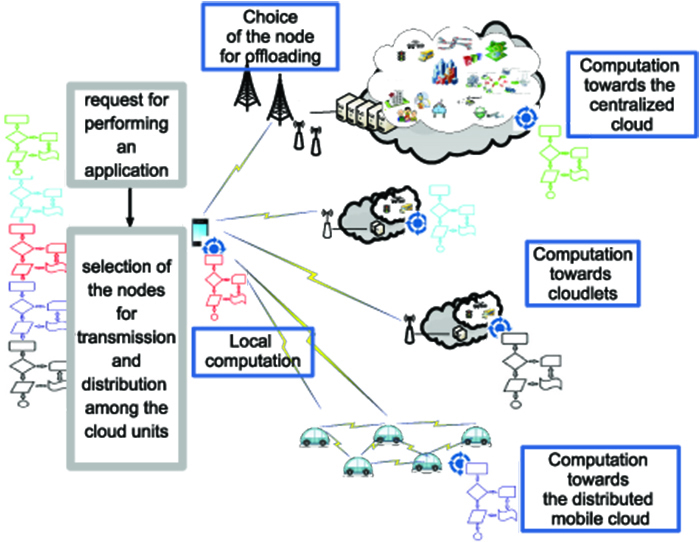
\includegraphics[width=\columnwidth]{offloading-distribution}
\caption{The process of distributing and performing the application among
different parts of the UMCC.}
\label{fig:offloading-distribution}
\end{figure}

Hence, when a \gls{RSMD} needs to select the clouds infrastructures to be used for computing the smart city application, we must focus on two main elements: 
\begin{itemize}
\item{the processing and storage devices - smart mobiles, \textit{per se} or together forming distributed mobile clouds, and cloud servers, constituting the cloudlets and the centralized cloud;}
\item{the wireless transmission equipments, - different \gls{RAT} nodes entailing diverse transmission speeds in relation to their own channel capacity and to the number of linked devices.} 
\end{itemize}

In \autoref{fig:offloading-distribution}, the  \gls{UMCC} framework is sketched by representing the functional flows of the architecture. Whenever a smart city application should be performed, the citizen within the \gls{UMCC} can select among different \gls{MCC} infrastructures, i.e., centralized clouds, cloudlets, and distributed mobile clouds, aiming to respect the requirements of the specific application depending on their features. 
The distribution depends on the application requirements, and the \gls{UMCC} features; its optimization will be discussed in the Section \ref{sec:cost}.
\subsection*{Computation, storage, and tranmission features}  
The features of the selected processing and storage devices, considered \textit{per se} or in a group forming cloud/cloudlets, are: 
\begin{itemize}
\item \emph{Processing Speed}: The processing speed corresponds to the performance speed of a device or a group of devices for processing the applications;
\item \emph{Storage Capacity}: The storage capacity corresponds to the amount of storage space provided by a device or a group of devices.
\end{itemize}
In the same time, the features of the transmission equipments to be taken into account are:
\begin{itemize}
\item \emph{Channel Capacity}: The nominal bandwidth of a certain communication technology that can be accessed by a certain device;
\item \emph{Priority/QoS management}: The ability of a certain communication technology to manage different \gls{QoS} and/or priority levels;
\item \emph{Communication interfaces}: The number of communication interfaces of each device, that impacts on the possibility of selection among the available heterogeneous networks.
\end{itemize}

\section{The UMCC model}
\label{sec:SystemModel}
In this paragraph we focus on the different entities playing a role in the \gls{UMCC} framework, describing the functions and the interactions among them. First of all, we are focusing on an application $\emph{App}$ requested by a \gls{RSMD}, defined through the number of operation to be executed, $O$, the amount of data to be exchanged, $D$, and the amount of data to be stored, $S$. An application can be seen as a smart city service, that can be executed either locally or remotely by exploiting the cloud infrastructures. Furthermore, each application has many requirements regarding the levels of \gls{QoS}. We have taken into account the following:
\begin{itemize}
\item the maximum accepted latency $T_\textit{app}$, intended as the interval between the request of performing an application and the acquisition of its results by the \gls{RSMD},
\item the minimum level of energy consumption $E_\textit{app}$, that the \gls{RSMD} necessarily uses for performing the application itself,
\item the throughput $\eta_\textit{app}$, intended as the minimum bandwidth that the application needs for being performed.
\end{itemize}
Hence, for highlighting the $\textit{App}$ dependence from the above measures, we can write: 
\begin{equation} 
\label{eq:App}
\emph{App} = \emph{App}(O,D,S,T_\textit{app},E_\textit{app},\eta_\textit{app})
\end{equation} 
%
A foundamental entity acting in the system is the \gls{RSMD} requesting the $\textit{App}$, we named $\textit{Dev}$, characterized by certain features that are involved in the offloading operation: the power to compute applications locally, $P_l$, the power used for transferring data towards clouds, $P_{\textit{tr}}$, the power for idling during the computation in the cloud, $P_{\textit{id}}$, the computing speed to perform locally the computation, $f_{\textit{l}}$, and the storage availability, $H_{\textit{l}}$. Furthermore, also the time-varying position of the device plays an important role in the system interactions. Hence, we can write:
\begin{equation}  
Dev = Dev(P_l, P_{\textit{tr}}, P_{\textit{id}}, f_{\textit{l}}, H_{l}, pos_{\textit{dev}}(x, y))
\label{eq:Dev}
\end{equation} 
Focusing on the different types of cloud entities in our scenario, we considered a unique centralized cloud $C_{\textit{cc}}$ and various cloudlets $C_{\textit{cl}}$ characterized by their own computing speed to perform the computation, i.e., $f_\textit{cc}$  for the centralized cloud and  $f_\textit{cl}$  for the cloudlets. Additionally, the storage availability  $H_\textit{cl}$ of each cloudlet has to be taken in consideration, while the storage availability of the centralized cloud can be considered infinite, therefore not constraining in the interaction. Hence, we can write for the centralized cloud $C_{\textit{cc}}$:
\begin{equation}
\label{eq:Ccc}
C_{\textit{cc}} = C_{\textit{cc}}(f_{\textit{cc}})
\end{equation} 
and for each cloudlet, considering also the influence of the position $pos_\textit{cl}(x, y)$ of the in-built \gls{AP}, the end-to-end throughput $\eta_{\textit{cl}}$ provided by the \gls{AP} itself, the maximum number of devices that it is possible to connect at the same time $n_\textit{cl}$, and the range of action $ r_{\textit{cl}}$: 
\begin{equation}
\label{eq:Ccl}
C_{\textit{cl}} = C_{\textit{cl}}(f_{\textit{cl}}, H_{\textit{cl}},  pos_{\textit{cl}}(x, y), \eta_{\textit{cl}}, n_\textit{cl}, r_{\textit{cl}})
\end{equation} 
We are considering the system from the point of view 
of a single \gls{RSMD} requesting to run an application, while the set of the other \glspl{SMD} constituting the distributed cloud are providing a service for supporting the  \gls{RSMD}.  
Thus, the distributed cloud is a set of generic entities $\textit{MD}s$, each characterized by its specific connectivity, computation and storage for the exchange of data, i.e. the computing speed $f_{\textit{MD}}$, the storage availability $H_{\textit{MD}}$, the position $pos_{\textit{MD}}(x, y)$, the throughput $\eta_{\textit{MD}}$, the number of devices that can be connected to each device$n_{\textit{MD}}$,  and each range of action $r_{\textit{MD}}$. 
Thus, we can write for the generic device $\textit{MD}$:
\begin{equation}  
\label{eq:SMD}
\textit{MD} = \textit{MD}( f_{\textit{MD}}, H_{\textit{MD}}, pos_{\textit{MD}}(x, y), \eta_{\textit{MD}} ,  n_{\textit{MD}},  r_{\textit{MD}} )
\end{equation}
    
While the connection to the cloudlets can be made only through the unique \gls{AP} that can be considered built-in in each cloudlet itself, and the connection of the distributed cloud to the \gls{RSMD} can be made directly, the nodes of the \gls{HetNet} offer different choices to connect towards the centralized cloud. Thus, for each involved node $\textit{Nod}$ constituting the centralized cloud, specifying that $pos_\textit{Nod}(x,y)$ is the position of the node, $\eta_\textit{Nod}$ is the end-to-end throughput in bit per second  between the user and the exploited node, $n_\textit{Nod}$ is the number of devices available to connect, and $r_\textit{Nod}$ is the range of availability of the node, we can write:
\begin{equation}
\label{eq:Nod}
\textit{Nod} = \textit{Nod}(pos_{\textit{Nod}}(x, y), \eta_{\text{Nod}} ,  n_{\text{Nod}},  r_{\text{Nod}})
\end{equation} 

The \autoref{tab:entities} summarizes the entities and the characteristics above described. 
\begin{sidewaystable}[tbp]
\renewcommand{\arraystretch}{2}
\begin{center}
\caption{Summary of entities and relations in the UMCC - Involved features and requirements}
\label{tab:entities}
{\begin{tabular}{l||c|c|c|c|cl}
Entity     & Connectivity	& Storage & Throughput & Energy	& Time latency 	\\  \hline
Reference Equation     &  	& \ref{eq:storage} & \ref{eq:throughput} & \ref{eq:energy}	& \ref{eq:latency} 	\\  \hline

$App = App(O,D,S,T_\textit{app},E_\textit{app},\eta_\textit{app})$		        & - 						& $S$ &	 $\eta_\textit{app}$ & $O$, $D$, $E_\textit{app}$					& $O$,$D$, $T_\textit{app}$		\\ 
$Dev = Dev(P_l, P_{\textit{tr}}, P_{\textit{id}}, f_{\textit{l}}, H_{l}, pos_{\textit{dev}}(x, y))$			& $pos_{\textit{dev}}(x, y)$	& $H_l$	&	-	& $P_l$, $P_\textit{tr}$, $P_\textit{id}$, $f_l$		& $f_l$				\\ 
$C_{\textit{cc}} = C_{\textit{cc}}(f_{\textit{cc}})$		& -			  				& -		&  - & $f_\textit{cc}$							& $f_\textit{cc}$				\\
$C_{\textit{cl}} = C_{\textit{cl}}(f_{\textit{cl}}, H_{\textit{cl}},  pos_{\textit{cl}}(x, y), \eta_{\textit{cl}}, n_\textit{cl}, r_{\textit{cl}})$		& $pos_{\textit{cl}}(x, y)$, $n_\textit{cl}$, $r_\textit{cl}$		& $H_\textit{cl}$ &	$\eta_\textit{cl}$ & $f_\textit{cl}$, $\eta_\textit{cl}$		& $\eta_\textit{cl}$, $f_\textit{cl}$		\\ 
$\textit{MD} = \textit{MD}( f_{\textit{MD}}, H_{\textit{MD}}$,$pos_{\textit{MD}}(x, y), \eta_{\text{MD}} ,  n_{\text{MD}},  r_{\text{MD}} )$		& $pos_{\textit{MD}}(x, y)$, $n_\textit{MD}$, $r_\textit{MD}$		& $H_\textit{MD}$ 	  &	$\eta_\textit{MD}$	& $f_\textit{MD}$, $\eta_\textit{MD}$	& $\eta_\textit{MD}$, $f_\textit{MD}$	\\ 
$\textit{Nod} = \textit{Nod}(pos_{\textit{Nod}}(x, y), \eta_{\text{Nod}} ,  n_{\text{Nod}},  r_{\text{Nod}})$		& $pos_{\textit{Nod}}(x, y)$, $n_\textit{Nod}$, $r_\textit{Nod}$	 		& -		&$\eta_\textit{Nod}$	& $\eta_\textit{Nod}$ 		& $\eta_\textit{Nod}$			\\ \hline
\end{tabular}}
\end{center}
\end{sidewaystable}
They are in a certain relationship due to some physical and logical constraints derived from the following considerations. 

First, for distributing the computation of the application among the different types of clouds, the system has to evaluate which \gls{HetNet} nodes, cloudlets, and \glspl{SMD} are available. The availability is realized if the \gls{RSMD} is in the range of action of a particular \gls{HetNet} node, cloudlet or \gls{SMD} and if these entities are not busy, i.e., if the number of devices connected to an entity $n_\text{conn}$ is less than $n_\textit{Nod}$, $n_\textit{cl}$, or $n_\textit{MD}$, dependently from the type of entity.
%, as shown in the Algorithm~\ref{alg1}.
%
%\begin{algorithm}[tbp]
%
%\begin{boxedalgorithmic}
%\renewcommand{\algorithmiccomment}[1]{// #1}
%\STATE \textbf{Available Connections}\\
%\STATE Requesting 
%\STATE $App = App(O,D,S,T_\textit{app},E_\textit{app},\eta_\textit{app})$ 
%\STATE by $Dev = Dev(P_l, P_{\textit{tr}}, P_{\textit{id}}, f_{\textit{l}}, H_{l}, pos_{\textit{dev}}(x, y))$      
%\FORALL {$\textit{Nod[i]} = \textit{Nod}(pos_{\textit{Nod,i}}(x, y), \eta_{\text{Nod,i}} ,  n_{\text{Nod,i}},  r_{\text{Nod,i}})$}
%        \IF{$| pos_\textit{Nod,i}(x,y) - pos_{\textit{dev}}(x, y) | \le  r_\textit{Nod,i}$} 
%        	\IF{$n_\text{conn,i} < n_\textit{Nod,i}$}
%        		\STATE{$\textit{Nod[i]} = \textit{Available}$}  
%		\ENDIF
%        	\ELSE \STATE{$\textit{Nod[i]} = \textit{Not-available}$} 
%        \ENDIF
%\ENDFOR
%\FORALL {$C_{\textit{cl}}[j] = C_{\textit{cl}}(f_{\textit{cl,j}}, H_{\textit{cl,j}},  pos_{\textit{cl,j}}(x, y), \eta_{\textit{cl,j}}, n_\textit{cl,j}, r_{\textit{cl,j}})$}
%        \IF{$| pos_{\textit{cl,j}}(x, y)) - pos_{\textit{dev}}(x, y) | \le r_{\textit{cl,j}}$} 
%        	\IF{$n_\text{conn,j} < n_\textit{cl,j}$}
%        		\STATE{$C_{\textit{cl}}[j] = \textit{Available}$}  
%		\ENDIF
%        	\ELSE \STATE{$C_{\textit{cl}}[j] = \textit{Not-available}$} 
%        \ENDIF
%\ENDFOR        
%\FORALL {\begin{multline}  
%\textit{MD[k]} = \textit{MD}(f_{\textit{MD,k}}, \notag  \\
% H_{\textit{MD,k}}, pos_{\textit{MD,k}}(x, y), \eta_{\text{MD,k}} ,  n_{\text{MD,k}},  r_{\text{MD,k}} )  \notag 
%\end{multline}   }
%        \IF{$| pos_{\textit{MD,k}}(x, y) - pos_{\textit{dev}}(x, y) | \le r_\textit{MD,k}$} 
%		\IF{$n_\text{conn,k} < n_\textit{MD,k}$}
%        		\STATE{$\textit{MD[k]} = \textit{Available}$}  
%		\ENDIF
%        	\ELSE \STATE{$\textit{MD[k]} = \textit{Not-available}$} 
%        \ENDIF
%\ENDFOR        
%\STATE
%\end{boxedalgorithmic}
%\caption{Available Connections}
%\label{alg1} 
%\end{algorithm}

%This algorithm permits 
%the detection of 
Thus, there are $M$ available \gls{HetNet} nodes $\textit{Nod}$ for offloading towards the centralized cloud,  $N$ cloudlets $C_{\textit{cl}}$ and $K$ devices $\textit{MD}$, able to share the computation in the distributed cloud.
After the detection of the available entities (which are a total of $1+M+N+K$, including the local node \gls{RSMD}, which we consider for simplicity the node of index 0), the next step is to distribute, by means of all these entities, different percentages $\alpha_i$  of operations $O$, $\beta_i$ of data $D$, and $\gamma_i$ of memory $S$, to all the available nodes, cloudlets and devices, under the constraints:
\begin{equation}
\label{eq:alpha}
\sum_{i=0}^\textit{M+N+K} \alpha_i = 1
\end{equation}
and
\begin{equation}
\label{eq:beta}
\sum_{i=1}^\textit{M+N+K} \beta_i = 1
\end{equation}
Alongside the computing capacity, it is possible to define a constraint regarding the storage availability of the cloudlets and the \glspl{SMD} by means of the following equations, considering infinite the storage availability of the centralized cloud:
\begin{equation}
\label{eq:storage}
\gamma_i S \le H_i \quad \quad \forall i \in \{0,1,...,i,..., \textit{N+K}\}
\end{equation}
that stands for an upper limit of remotely used storage of a certain $i$-th cloud infrastructure.

A constraint related to the application's requirements $\eta_\textit{app}$ involves the throughput of the entities designated for the offloading: the overall throughput offered by the selected devices should be higher than the minimum throughput requirement of a certain application:
 \begin{equation}
\label{eq:throughput}
\sum_{i=1}^\textit{M+N+K} \eta_i \ge \eta_\textit{app}
\end{equation}
From the point of view of the \gls{RSMD}, the energy spent for offloading the application can be written as the sum of the energy spent to perform locally a part of the task, plus the energy spent by the \gls{RSMD} for the transmission of data to the clouds, plus the energy spent during the idle period when the computation is being offloaded. 
Hence, the restriction related to the requirement $E_\textit{app}$ leads to the following:
\begin{equation}
\label{eq:energy}
P_l \frac{\alpha_0 O}{f_l}  + \sum_{i=1}^\textit{M+N+K}{P_\textit{tr}\frac{ \beta_i D}{\eta_i} + P_\textit{id}  \operatorname*{arg\,max}_{i =1,\textit{M+N+K}}\left \{ \frac{\alpha_i O }{f_i} \right \}}\le{E_\textit{app}}
\end{equation}
In the same time, the total latency is the sum of the time for computing locally the $\alpha_0$ percentage of computation, plus the times to transmit/receive data to/from the other computation units, plus the maximum of the time to compute in offloading. Hence, the restriction related to the requirement $T_\textit{app}$ leads to the following:
\begin{equation}
\label{eq:latency}
%T=t_l^{\text{comp}}+t_{cc}^{\text{tr}}+t_{cc}^{\text{comp}}+t_{cl_j}^{\text{tr}}+t_{cl}^{\text{comp}}+t_{dc_j}^{\text{tr}}+t_{dc}^{\text{comp}}\\
\alpha_0 \frac{O}{f_l}+ \sum_{i=1}^\textit{M+N+K} \frac{ \beta_i D}{\eta_i} +  \operatorname*{arg\,max}_{i =1,\textit{M+N+K}}\left \{ \frac{\alpha_i O }{f_i} \right \}\le{T_\textit{app}}
\end{equation}
Furthermore, the throughput $\eta_i$ is related to the number of devices $n_i$ connected to the $i^{th}$ entity and the channel capacity $BW_i$ as shown by the following representing the Shannon Formula:
\begin{equation}
\eta_i = \frac{\textit{BW}_i}{n_i}\cdot \log_2{\left(1+\frac{\textit{SNR}_i}{d_i^2}\right)}
\label{eq:shannon1}
\end{equation} 
where $\textit{SNR}_i$ is the \gls{SNR} of the related link and $d_i$ the distance between the receiver and the transmitter. Thus, the optimization of the system consists in finding the values of $\alpha_i$, $\beta_i$ and $\gamma_i$ that satisfy eqs.~\eqref{eq:alpha}-(\ref{eq:shannon1}). This is a nontrivial optimization problem, but the complexity can be decreased with the introduction of some simplifications, as presented in the following chapters.


\section{Requirements of smart city applications}
\label{sec:requirements}
There are many taxonomies trying to define smart city key areas, where social aims, care for environment, and economic issues are related and interconnected. 
The \gls{IERC} has identified in~\cite{IERC} a list of applications in different domains of \gls{IoT}, including the smart city domain, showing the utmost strategic technology trends for the next five years. 
Moreover, the Net!Works European Technology Platform for Communications Networks and Services has issued a white paper~\cite{whitepaperNetWorks} aiming to identify the major topics of smart cities that will influence the \gls{ICT} environment. 
Furthermore, a relevant document aiming to categorize and define the different applications has been released by \gls{ETSI}, where several application types have been specified focusing on their bandwidth requirements~\cite{etsi}. 

Taking into account all the relevant observations presented in these essays, we analyzed some particular smart city applications covering the areas of mobility, healthcare, disaster recovery, energy, waste management and tourism, in order to leverage the \gls{UMCC} identifying the requirements which are related to the \gls{QoS}.

Each application is defined through the service provided to the citizens, concerning the requirements in terms of throughput, energy consumption, time due to the transferring and computation processes, and number of users. 
In addition, for every application, the typical requirements of processing, data to exchange and storage have been established. The following list summarizes the definition of these requirements:
\begin{itemize}
	\item \emph{Latency}: The latency is defined as the amount of time required by a certain application between the event happens and the event is acquired by the system;
	\item \emph{Energy Consumption}: The energy consumption corresponds to the energy consumed for executing a certain application locally or remotely;
	\item \emph{Throughput}: The throughput corresponds to the amount of bandwidth required by a specific application to be reliably installed in the smart city environment;
	\item \emph{Computing}: The computing corresponds to the amount of computing process requested by a certain application;
	\item \emph{Exchanged data}: The exchanged data correspond to the amount of input, output and code information to be transferred by means of the wireless network; 
	\item \emph{Storage}: The storage corresponds to the amount of storage space required for storing the sensed data and/or the processing application;
	\item \emph{Users}: The users correspond to the number of users for achieving a reliable service.
\end{itemize}

The \gls{QoS} is a function of the previous requirements, where each one of these plays a role less or more important depending on the aims of the application. 
In the following list the considered application types are described by highlighting their technological requirements and characteristics, while in \autoref{tab:applications1} the considered application types and the significance of their requirements are summarized.
\begin{sidewaystable}
\renewcommand{\arraystretch}{2}
\centering
\caption{Summary of smart city applications and Requirements}
\label{tab:applications1}
{\begin{tabular}{c||c|c|c|c|c|c|c|}
& \multicolumn{7}{c|}{Requirements}\\\hline\hline
Application 		& latency 	 		& energy			& throughput 		& computing 	& exchanged data 	& storage   & users\\  \hline
Mobility 			& restrictive 		& variable			& restrictive		& high		& high			& variable	 & high	\\ 
Healthcare			& restrictive  	& non-restrictive 	& non-restrictive		& high			& high			& high		 & low	\\
Disaster Recovery	& restrictive 	& restrictive 		& non-restrictive		& high			& high			& high	 & variable	\\
Energy			& non-restrictive	& non-restrictive		& non-restrictive		& high			& high			& high	 & high	\\ 
Waste Management	& non-restrictive	& restrictive		& non-restrictive 	& low 			& low			& low	& low	\\
Tourism			& non-restrictive	& restrictive	& non-restrictive 	& high	& high	& high	& variable	\\
\hline
\end{tabular}
}
\end{sidewaystable}

\paragraph{Mobility}
All the components in an intelligent transportation system could be connected to improve transportation safety, relieve traffic congestion, reduce air pollution and enhance comfort of driving. 
The three-layered hierarchical cloud architecture for vehicular networks proposed by Yu et al.~\cite{Vehicular}, where vehicles are mobile nodes that exploit cloud resources and services, can be considered as included in the \gls{UMCC} framework. 
A real-time navigation with computation resource sharing, where the computation resources in the central cloud are utilized for data traffic mining, requests a minimal latency, since a ready response is needed. 
On the other hand, considering that the great part of mobile devices can be recharged directly from the car, energy consumption has to be considered only for pedestrians and bicycles. 
The necessary throughput, the computational load and the amount of data to exchange are high, whereas we can think the storage as a secondary requirement, unless for security recording.  

\paragraph{Healthcare}
Intelligent and connected medical devices, monitoring physical activity and providing efficient therapy management by using patients' personal devices, could be connected to medical archives and provide information for medical diagnosis. We considered in the \gls{UMCC} framework the typical architecture proposed by He et al.~\cite{HEALTH}, requiring a full integration of the clinical devices and efficient processing of the collected data, considering, for instance, a cloudlet nearby the home of the patient. 
In this case there are relatively low requirements regarding energy consumption, throughput and number of users, whereas the requirements of latency, computation, exchanged data and storage are high, considering the complexity of the management algorithm, the video monitoring for remote diagnosis and the data to store for the personal record archive.

\paragraph{Disaster Recovery}
In~\cite{Satyanarayanan} a disaster relief scenario is described, where people are facing with the destruction of the infrastructures and local citizens are asked to use their mobile phones to photograph the site. 
Also this case introduces the three-layered cloud described in the \gls{UMCC} framework, requiring to transmit a lot of data using the cameras provided by the smartphones to reconstruct the disaster scene. 
In this case there are relatively low requirements regarding throughput, whereas it is important to have a quick response and to save the energy of the devices. 
There are a lot of computation to reconstruct the scene and a lot of data to exchange and to store. 
The number of users is variable.

\paragraph{Energy}
Energy saving can take advantage from the cloud basically thanks to smart grid systems, aimed to transform the behavior of individuals and communities towards a more efficient and greener use of electric power.
Data fusion and mining, as well as scheduling and optimization, are critical in order to include the use of wireless communications to collect and exchange information about electric quality, consumption, and pricing in a secure and reliable fashion. 
By analyzing the specific aspects regarding the \gls{UMCC}, if we consider an application where vehicles are involved in a smart grid system, we can suppose that a big data exchange is needed, there is a lot of computation and storage between a large number of users, whereas there are relatively low requirements regarding latency and throughput, and energy saving is not a problem for the devices involved.

\paragraph{Waste Management}
Automatically generated schedules and optimized routes which take into account an extensive set of parameters (future fill-level projections, truck availability, traffic information, road restrictions, etc.) could be planned not only looking at the current situation, but also considering the future outlook. 
A logistic solution that uses wireless sensors to measure and forecast the fill-level of waste and recycling containers could combine fill-level forecasts with an extensive set of collection parameters (e.g., traffic information, vehicle information, road restrictions) in order to calculate the most cost efficient collection plan. 
This smart plan would be automatically generated and accessed by the driver through a tablet\footnote{Example from \url{http://www.enevo.com/}}. 
We can expect non-restrictive requirements of latency and throughput, whereas  resource-poor equipments have to be taken into consideration. 
The requirements related to data to be exchanged, load of computation, storage and number of users are not critical.

\paragraph{Tourism}
Augmented reality and social networks are the characteristics of applications that more take advantage from the cloud, that becomes also useful for mobile users sharing photos and video clips, tagging their friends in popular social networks like Twitter and Facebook. 
The cloud is effective also when mobile users require searching services, also using recognition techniques (using voice, images and keywords)\footnote{Example from \url{http://www.mtrip.com/augmented-reality/}}. 
We can expect not-restrictive requirements of latency and throughput, whereas  resource-poor equipments have to be taken into consideration. 
There are a great amount of data to be exchanged, load of computation and storage and number of users are variable.

\section{A utility based resource optimization approach}
\label{sec:cost}
The requirements related to the applications, and the associated \gls{QoS}, can be respected by optimizing the application partitioning and node/cloud association based on the features of the processing and storage devices and of the transmission equipments introduced in \autoref{sec:challenges}. Moreover, it should be noted that there is a correlation among the application requirements and the features of the \gls{UMCC} equipments. 

The latency suffered to perform a certain application can be seen as composed by the time needed for transferring the application data to the cloud computing infrastructure and the time needed for the cloud computation, therefore it is affected by the processing speed of the involved devices and by the channel capacity and the communication interfaces of the chosen transmission equipments. 
Furthermore, the energy spent to perform an application depends on the time needed for the data transfer, thus it depends on the channel capacity and the number of communication interfaces of the communication equipments; it has to be noticed that we have to consider also the energy spent by the user device while idles during the cloud computation, so that the processing speeds of the cloud devices are involved. 
The storage value of the application does not influence directly the performance of the system, but it can represent a limitation for the usability of a certain cloud infrastructure, as well as the number of potential users of the application.
% by the system, we focus here on the energy spent by the mobile devices, by neglecting the energy spent on the centralized cloud and the cloudlet infrastructures; it has to be noticed that we have to consider also the energy spent during the idle period by the user devices corresponding to the time needed by the cloud to perform the computation: we suppose that during this time the user device remains in an idle state. The bandwidth is affected by the channel capacity of the selected wireless network and by the number of users connected. The storage value does not influence directly the performance of the system, but it can represent a limitation for the usability of a certain cloud infrastructure, as well as the number of potential users of the application.

A feasible optimization regarding the computing and the exchanged data requirements can be performed by operating on the complexity of the computability resources, considering also that, in partial offloading, the exchanged data could not be a predetermined value~\cite{Challenges}. 

In this context, a utility function aiming to optimize the application-dependent \gls{QoS} is proposed, acting as input for a procedure of partition and a node/cloud association, as shown in \autoref{fig:FunctionalBlocks}. The utility function can be written as:
\begin{equation}
U =  \sum_{i=1}^{N_{req}}\gamma_i f_i(\xi_i)
\label{eq:global-utility}
\end{equation}
where $N_{req}$ is the number of requirements for a certain smart city application, $\xi_i$ stands for the $i$-th application requirement among those defined in \autoref{sec:requirements}, and $\gamma_i$ is a weight value, while $f_i(\cdot)$ corresponds to a specific utility function used for evaluate the respect of the $i$-th requirement. 

In \autoref{fig:FunctionalBlocks}, the functional blocks of the \gls{UMCC} framework, based on a utility function optimization, are represented. 
On one hand, the smart city applications define specific requirements, while the cloud topologies in a certain scenario set their features. 
The utility function aims at selecting those cloud topologies that allow to respect the requirements by setting an optimized distribution of the application itself. 
The optimization of the partition and the node association will impact again on the \gls{UMCC} features to be used by the other applications.

\begin{figure}[tbp]
\centering
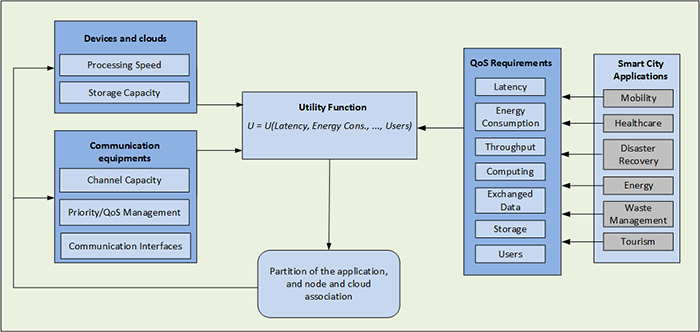
\includegraphics[width=\columnwidth]{FunctionalBlocks.png}
\caption{The utility function acts for distributing and performing the application in different parts of the Urban MCC.}
\label{fig:FunctionalBlocks}
\end{figure}

The maximization of the introduced utility function could be a nontrivial optimization problem, depending on the considered number of applications and devices acting in the selected scenario. 
In relation to the introduced requirements, the number of constraints could be reduced, and the complexity of the problem decreased by introducing opportunely defined sub-optimal solutions. 
All the utility and cost functions presented in the following chapters are particular cases of the \autoref{eq:global-utility}. 
In particular, in \autoref{chap:EUCNC}  a cost function including the tradeoff between energy consumption of mobile devices versus the time to offloading data and to compute tasks on a centralized remote cloud server is provided, evaluating the optimal offloading fraction depending on the network’s load; in \autoref{chap:GLOBECOM14} and in \autoref{chap:socialBRA} we focused on a utility function representing the \gls{QoS} degree perceived by the user, modeled as a sigmoid curve, that is a well-known function often used to describe \gls{QoS} perception~\cite{Badia}; finally, in \autoref{chap:cluster-based} we focused on the computation offloading towards the distributed cloud, for offloading a real-time navigation application in a distributed fashion, aiming to minimize the execution time, since the devices are autonomous regarding the energy provision. 
%The function is modeled as a sigmoid curve, that is a well-known function often used to describe \gls{QoS} perception~\cite{Badia}. 
%A sigmoid curve can be defined as:
%$$
%f(x)=\frac{1}{1+e^{-\alpha (x-\beta)}}
%$$
%where $\alpha$ and $\beta$ decide the steepness and the center of the curve. 
%The value of $\alpha$ indicates user's sensitivity to the \gls{QoS} degradation while $\beta$ indicates the \emph{acceptable} region of operation. 
%The derivative of the sigmoid function describes the subject perception, so that it does not make sense to give more resources over a certain value above which the derivative of the utility function approximate to zero.
%
%In particular in~\cite{Globecom2014} the focus was on a selected subset of smart city applications whose most restrictive requirements are energy consumption, latency and throughput. 
%The  defined utility function can be used for a cell association scheme that allows the selection by each smart city device of the \emph{best} access point for respecting the requirements of the considered applications; whenever an application should be computed, the utility function is evaluated aiming to respect the requirements. 
%

\section{Conclusions}
\label{sec:conclusions1}
In this chapter we introduced the \gls{UMCC} framework, a concept that supports the smart city vision for the optimization of the \gls{QoS} of various types of smart city applications. 
The \gls{UMCC} consists of different topologies of cloud and diverse types of \glspl{RAT}, that are used for offloading computation and share resources among the mobile devices. 
The \gls{QoS} depends on the type of application, since it is affected by the defined requirements in a different way depending on the aims of the application itself. 
A cost function optimization approach is proposed, aiming to select the optimal partition level of the applications and the cloud infrastructures to be used for their computation. 
The optimization of the \gls{QoS} is influenced by a big number of features, related to the choice of the distribution of data in the cloud units and the nodes used for the transmission, but the problem can be restricted considering some simplifications suggested by the aims and the domain of the application. 

\part{Partial Offloading Optimization}
A \gls{UMCC} framework settled on an efficient wireless network allows users to benefit from multimedia services in an ubiquitous, seamless and interoperable way. 
In this context \gls{MCC} and \glspl{HetNet} are viewed as infrastructures providing together a key solution for the major facing problems: the former allows to offload application to powerful remote servers, shortening execution time and extending battery life of mobile devices, while the latter allows the use of small cells in addition to macrocells, exploiting high-speed and stable connectivity in an ever grown mobile traffic trend.
In order to fulfill the computation offloading efficiently, in the following chapters we explore techniques aiming to move the computing application towards the cloud, considering a non-trivial multi-objective optimization approach that takes into consideration the tradeoff between the energy consumption of the \glspl{SMD} and the time for executing the application. 
The aim of the optimization is to find the percentage of application offloading  that minimizes the proposed cost function, in such a way that only a part of the application is transfered and computed outside, whereas the rest of the application is computed locally.

The \autoref{chap:EUCNC} deals with the partial offloading technique in a \emph{centralized cloud} scenario.
The results show that exists a particular offloading percentage value fitting the system in case of simultaneously high data and network workload, differently from the simple \emph{yes/no} offloading decision which would move the entire application or would perform it locally. 
In \autoref{chap:GLOBECOM14} the partial offloading technique is applied using a utility function model arising from the economic world. It aims to measure the \gls{QoS}, in order to choose the best \gls{AP} in a \gls{HetNet} for running the partial computation offloading. The goal is to save energy for the \glspl{SMD} and to reduce computational time. 
In \autoref{chap:cluster-based} the proposed \gls{UMCC} framework and the partial computation offloading are applied to a vehicular environment for handling a real-time navigation application. In this case, we consider also cloudlets and distributed clouds, so that the \glspl{SMD} can exploit road side units and other neighbor devices for delegating a shared application.

\vspace{1cm}
\textit{The content of the following chapters was extracted from publications \hyperref[P3]{[P3]},  \hyperref[P4]{[P4]}, and \hyperref[P5]{[P5]}.}

\chapter[A Partial Computation Offloading Technique]{A Partial Computation Offloading\\ Technique}
\label{chap:EUCNC}
\section{Introduction}
Smart cities are considered a paradigm where wireless communication is an enhancing factor to make better urban services and improve the quality of life for citizens and visitors. 
In a smart city scenario several entities should be taken into consideration: the wireless infrastructure that allows data-exchange, the user devices, the sensing nodes, the machine devices, access points, one or more cloud infrastructures. 
Moreover, for delivering the requested services lots of data are exchanged among the citizens and the devices, and these data need also to be elaborated in order to give the correct information to the users.
Thanks to various wireless communication technologies, users can move through different environments, indoor and outdoor, providing data to the cloud and receiving access services as browsing, video on demand, video streaming, information about location and maps. 
In this context, energy saving and performance improvement of the \glspl{SMD} have been widely recognized as primary issues. 
In fact, the execution of every complex application is a big challenge due to the limited battery power and computation capacity of the mobile devices, especially in a smart environment where communication is considered a key to get better features in important areas such as mobility and transportation. 

The exploitation of \gls{HetNet} infrastructures together with the opportunity to delegate computation load to \gls{MCC}, as shown in \autoref{fig:HetNet_MCC},  is an appealing connection achieving the aims of saving the \gls{SMD}'s power resource and executing the requested tasks in a faster way~\cite{Challenges}.
\begin{figure}[tbp]
\centering
\includegraphics[width=1\columnwidth]{HetNet_MCC}
\caption{The reference scenario with access nodes in HetNet for Mobile Cloud Computing}
\label{fig:HetNet_MCC}
\end{figure}
\glspl{HetNet} involve multiple types of low power radio access nodes in addition to the traditional macrocell nodes in a wireless network, reaching the major goal to enhance connectivity. On the other hand, \gls{MCC} aims to increase the computing capabilities of mobile devices, to conserve local resources - especially battery charge - to extend storage capacity and to enhance data safety for making the computing experience of mobile users better~\cite{Cloud-based}.

The distributed execution (i.e., computation/code offloading) between the cloud and mobile devices has been widely investigated~\cite{DinhSurvey}, highlighting the challenges towards a more efficient cloud-based offloading framework and also suggesting some opportunities that may be exploited.
Indeed, the joint optimization of \glspl{HetNet} and distributed processing is a promising research trend~\cite{fantacci09}.

Several works have already analyzed characteristics and capacity of \gls{MCC} offloading, for example aiming to extract offloading friendly parts of codes from existing applications~\cite{CuervoMAUI, CloneCloudChun}. 
Also, in~\cite{MobileMeetCloud} the key issues are identified when developing new applications which can effectively leverage cloud resources.  
Furthermore, in~\cite{Barbera} a real-life scenarios, where each device is associated to a software clone on the cloud, has been considered, and in~\cite{Murmuria} a system that effectively accounts for the power usage of all of the primary hardware subsystems on the phone has been implemented, distinguishing between CPU, display, graphics, GPS, audio, and microphone. 

In~\cite{Time-and-Energy-Aware} an offloading framework, named Ternary Decision Maker (TDM), has been developed, aiming to shorten response time and reduce energy consumption simultaneously with targets of execution including on-board CPU and GPU in addition to the cloud, from the point of view of the single device. 
In addition, there are many studies that focus on whether to offload computation to a server, providing solutions related to a yes/no decision for the entire task at one time~\cite{Kumar,Tradeoff}, or studies that focus on optimization of the energy consumption in \glspl{SMD} necessary to run a given application under execution time constraint~\cite{Barbarossa1}.

Differently from the literature, we propose a partial offloading technique able to exploit the \glspl{HetNet} scenario and the presence of \gls{MCC} devices - the \gls{UMCC} framework - by optimizing the amount of partial offloading of the computational tasks depending on the number of devices connected to a network and their location with respect to the \gls{WiFi} access points or \gls{LTE} eNodeBs.  
The \glspl{SMD} can exploit the partial data offloading to distribute high computational tasks among centralized servers and local computing.
 
In \autoref{fig:offloadingOrNot} the workflow and the entities involved in the performance of a task are shown. From the point of view of a single user, the decision about offloading or not is taken on the basis of the following considerations:
\begin{itemize}
\item If the task is delegated to the cloud, the energy consumed by the mobile device is due to the data transfer - uploading data and downloading results - plus the energy consumed in an idle state during the outside computation  - waiting for the results; the global time for having the task accomplished is related not only to the computational time but also to the transfer time for moving data from the mobile device to the cloud and \emph{vice-versa}.

\item If the task is computed locally, the energy consumed by the mobile device is due to the computation itself; the global time for having the task accomplished is related only to the computational ability of the \gls{SMD}.
\end{itemize}
\begin{figure}[tbp]
\centering
\includegraphics[width=\columnwidth]{offloadingOrNot}
\caption{The offloading decision from the point of view of a single user.}
\label{fig:offloadingOrNot}
\end{figure}

In this chapter the optimization of the entire system is considered, not for a single device but for the whole community of devices, by taking into account partial offloading in a non trivial multi-objective optimization approach, where both energy consumption and execution time constraints are considered. 
A cost function including the tradeoff between energy consumption of mobile devices versus the time to offloading data and to compute tasks on a remote cloud server is provided, evaluating the optimal offloading fraction depending on the network's load.
It can be exploited when the network is overloaded and the tasks  request large amounts both of computation to perform and data to exchange.  

\section{System Model}
The reference scenario is characterized by a urban area with a pervasive wireless coverage, where several mobile devices are interacting with a traditional centralized cloud and request for services from a remote data center, as illustrated in \autoref{fig:HetNet_MCC}.
Alongside the presence of a pervasive wireless network, the system deals with many sensing and user terminals that generate and exploit a large amount of data.
In order to connect the \glspl{SMD} to the cloud and the data centers for delegating data for the computation, we take into account a simple categorization of the \gls{UMCC}'s trasmission entities, considering only two types of \glspl{RAT} forming the basic elements of the \glspl{HetNet}: macrocells and small cells.
If, on one side, the strategy of delegating computation to the centralized cloud allows to exploit high performance computing centers, on the other side, 
it copes with the energy spent by the \glspl{SMD} for transferring data. 
Similarly, the \glspl{SMD} which compute locally the applications in a distributed approach, face with the energy issues due to the computation itself.
In other words, the \glspl{SMD} consumes energy  both to delegate the application to the data centers and to compute it locally.  Furthermore, both the speed to transmit data and the speed for local computation are related to the energy consumed by the \glspl{SMD}. Thus, the offloading decision between offloading the application or computing it locally leads to a tradeoff. 
For this reason our model provides a cost function by resorting to a previously introduced model in~\cite{Kumar,Tradeoff} which compares the energy used for a 100\% offloading with the ones used to perform the task locally. The parameters used in the following are listed in \autoref{tab:parameters}. 

	\begin{table}[tbp]
	\renewcommand{\arraystretch}{2}
	\begin{center}
	\caption{Offloading Parameters}
	\label{tab:parameters}
	{
	\begin{tabular}{l|p{2.5in}|p{2in}}\hline\hline
	{symbol}& {meaning}& {unit of measure}\\ \hline
	 
	$P_{l}$      &  power for local computing& W\\ 
	$P_{\textit{id}}$      &  power while being idle& W\\ 
	$P_{\textit{tr}}$      &  power for sending and receiving data& W\\ 
	 
	$S_{\textit{md}}$      &  SMD's calculation speed & no. of instructions / s\\ 
	$S_{\textit{tr}}$      &  SMD's transmission speed  & bit / s\\
	$S_{\textit{cs}}$      &  cloud server's calculation speed & no. of instructions / s\\ 
	
	$C$      &  instructions required by the task  & no. of instructions\\ 
	$D$      &  exchanged data  & bit\\ \hline
	\end{tabular}
	}
	\end{center}
	\end{table}
In our scenario we suppose that the computation of a certain task requires $C$ instructions.
 $S_{\textit{md}}$ and $S_{\textit{cs}}$ are, respectively, the speeds in instructions per second of the mobile device and the cloud server. 
Hence, a certain task can be completed in an amount of time equal to $C/S_{\textit{md}}$ on the device and $C/S_{\textit{cs}}$ on the server. 
On the other hand, let us suppose that $D$ corresponds to the amount of bits of data that the device and the server must exchange for the remote computation, and $S_{\textit{tr}}$ is the transmission speed, in bit per second between the \gls{SMD} and the access point; hence, the transmission of data lasts an amount of time equal to $D/S_{\textit{tr}}$. 
In this case we consider that the transmission time is mostly due to the access network transfer, because the transfer rate of the backbone network can be considered as negligible due to the higher data rate.
Moreover, we consider as negligible the transfer time from the access point to the user terminal because the amount of data in response to the elaboration in centralized server is little with respect to the data sent to the centralized server~\cite{Kumar,Tradeoff}.

Hence, it is possible to derive the energy for local computing:
	 \begin{equation}
	 \label{eq:E_locale}
	 E_{l} = P_{l}\times\frac{C}{S_{\textit{md}}} 
	 \end{equation}
as the product of the power consumption of the mobile device for computing locally, $P_{l}$, and the time $C/S_{\textit{md}}$ needed for the computation. Similarly, it is possible to derive the energy needed for performing the task computation on the cloud as the energy used while being in idle for the remote computation plus the energy used to transmit the whole data from the \gls{SMD} to the cloud:
\begin{equation}
	 \label{eq:E_OD100}
	 E_{\textit{od}} = P_{\textit{id}}\times\frac{C}{S_{\textit{cs}}} + P_{\textit{tr}}\times\frac{D}{S_{\textit{tr}}},
	 \end{equation}
%
where $P_{\textit{id}}$ and $P_{\textit{tr}}$ are the power consumptions of the mobile device, in watts, during idle and data transmission periods, respectively.
 
Similarly, it is possible to derive the time needed for the local computing as:
	\begin{equation}
	\label{eq:T_locale}
	T_{l} = \frac{C}{S_{\textit{md}}}, 
	\end{equation}
	and the time for the whole offloading computing as 
	\begin{equation}
	\label{eq:T_OD100}
	T_{\textit{od}} = \frac{C}{S_{\textit{cs}}} + \frac{D}{S_{\textit{tr}}}
	\end{equation}

In many applications, this approach is not efficient or feasible, and it is necessary to partition the application at a finer granularity into local and remote parts, which is a key step for offloading.	

\section{Adaptive Offloading}
In this section, firstly, two equations are provided, to represent the energy used by a \gls{SMD} to execute an application in partial offloading and to express the time needed to execute such application. 
Secondly, the impact of the traffic workload in the wireless network is taken into account, since the \glspl{RAT} and the number of \glspl{SMD} entails the transmission speed of the the offloading data. 
Thirdly, a cost function is introduced, to evaluate the percentage of offloading which minimizes both energy and time.

In order to analyze the energy spent for offloading only a part of the application, we introduce the weight coefficients ${\gamma}$ and ${\delta}$, satisfying ${0 \le \gamma ,\delta \le 1}$, representing respectively the percentage of the computational task and the percentage of the exchanged data for offloading. 
Then, the used energy of a single device ${E_{\textit{part}\_\textit{od}}}$ has been introduced, as the sum of the one spent to perform a part of the task locally plus the one spent to idle and transmit the other part of the task to the cloud:
	\begin{equation}
	E_{\textit{part}\_\textit{od}}  = P_{l}\times\frac{(1-\gamma)\cdot C}{S_{\textit{md}}} 
	+ P_{\textit{id}}\times\frac{\gamma\cdot C}{S_{\textit{cs}}} + P_{\textit{tr}}\times\frac{\delta\cdot D}{S_{\textit{tr}}}
	\label{eq:E_ODpart}
	\end{equation}

Taking into account the same coefficients $\gamma$ and $\delta$ used in \autoref{eq:E_ODpart}, we can calculate the time for the partial offloading ${T_{\textit{part}\_\textit{od}}}$ as  the maximum between the time needed for computing the local part of the task and the time needed for the offloading, considering the two phases performed in the same time:
	\begin{equation}
	\label{eq:T_ODpart}
	T_{\textit{part}\_\textit{od}} = \max \left(\frac{(1-\gamma)\cdot C}{S_{\textit{md}}};\quad\frac{\gamma\cdot C}{S_{\textit{cs}}} + \frac{\delta\cdot D}{S_{\textit{tr}}}\right)
	\end{equation}

The structure and the workload of the network are implicitly considered in \autoref{eq:E_ODpart} and \autoref{eq:T_ODpart}. 
Now we are going to describe the effect on ${E_{\textit{part}\_\textit{od}}}$ and ${T_{\textit{part}\_\textit{od}}}$ due to the different \glspl{RAT} performing in the \glspl{HetNet} and to the amount of devices connected to this different  \glspl{RAT}.
The \gls{HetNet} mainly consists of two components, macrocells and small cells, with different bandwidths ${\textit{BW}}$. 
Since, for a single \gls{SMD}, the speed rate of the data exchange ${S_{\textit{tr}}}$ is affected by the bandwidth of the node to which the \gls{SMD} is connected, by the distance ${d}$ from this node, and by the number ${n}$ of the overall \glspl{SMD} connected to the same node, ${S_{tr}}$ can be written in an explicit way as:
 	\begin{equation}
	\label{eq:Str}
	S_{tr} = \frac{\textit{BW}}{n}\cdot \log_2{\left(1+\frac{\textit{SNR}}{d^2}\right)}
	\end{equation}   
	where  $\textit{SNR}$ is the \gls{SNR}, typical parameter of the device.
 
In order to allow the evaluation of the offloading percentage, aiming to save energy and improve performance, the introduction of a cost function that can consider the minimization of both \autoref{eq:E_ODpart} and \autoref{eq:T_ODpart} for the entire set of \glspl{SMD} is required. 
This is a non-trivial multi-objective optimization problem that we addressed by setting the cost function as a weighted sum of both the average values, with $\alpha$ and $\beta$ coefficients with the constraints $0\le\alpha,\beta\le1$ and $\alpha+\beta=1$, $N$ number of network's devices and ${E_l}$, ${T_l}$ reference values representing average energy and time spent when the task is computed locally by a \gls{SMD}: 
 \begin{equation}
	\label{eq:FCost}
	F = \alpha \frac{\frac{1}{N}\sum_{k=1}^N E_{\textit{part}\_\textit{od},k}(\gamma,\delta)}{E_l} + \beta \frac{\frac{1}{N}\sum_{k=1}^N T_{\textit{part}\_\textit{od},k}(\gamma,\delta)}{T_l}
	\end{equation}            
This cost function is based on a network centric approach in which a central entity is responsible for choosing values of the offloading percentage $\gamma$ and $\delta$ after collecting informations about the \glspl{SMD}' features. 
Furthermore, in the partial offloading procedure, $\gamma$ and $\delta$ are bounds, because before a task is executed it may require certain amount of data from other tasks~\cite{Challenges}. 
Moreover, the weighted coefficients $\alpha$ and $\beta$ are chosen at a main level to give a major importance to energy or time saving.   

\section{Numerical Results}
During a partial offloading the amount of energy and time in \autoref{eq:E_ODpart} and \autoref{eq:T_ODpart} is affected by the percentage of computation and communication exchanged, represented respectively by the coefficients $\gamma$ and $\delta$. 
These are correlated each other, since the execution of a remote computation task requires a certain amount of input/output data to be exchanged. 
So we can consider the ratio $\frac{\delta}{\gamma}$ as a typical value, peculiar of a type of application. To summarize typical scenarios we have taken into account three kinds of applications represented in \autoref{tab:Apps}, according to the aims to analyze cases of a smart transportation system~\cite{TowardCloudBased}.
 
\begin{table}[tbp]

\begin{center}
\caption{Application Types}
\label{tab:Apps}
{
\renewcommand{\arraystretch}{2}
\begin{tabular}{p{2in}|p{1in}|p{1in}|c|c|c}\hline\hline 
Application & Computation & Data transmission & $C$ & $D$ & $\delta/\gamma$\\  \hline
1 - Real time traffic analysis &  High & Low &  $10^7$ & $10^5$ & $0.25$\\
2 - Mobile Video and Audio Communication &  Low & High &  $10^5$ & $10^7$ & $0.75$\\ 
3 - Mobile Social Networking &  High & High &  $10^7$ & $10^7$ & $0.50$\\ \hline
\end{tabular}
}
\end{center}
\end{table}

We considered a deployment area of $1000\times1000\ m^2$, where one \gls{LTE} eNodeB with channel capacity equal to 100 MHz and three \gls{WiFi} access point with channel capacities equal to 22 MHz are positioned to cover the entire area. 
Specifically, the access points are positioned at point (0,0), (500,1000) and (0,1000), and the LTE station at (500,500), as shown in \autoref{fig:env}. 

\begin{figure}[tbp]%
\centering
\subfloat{\includegraphics[width=0.7\columnwidth]{ENV500}}\\
\subfloat{\includegraphics[width=0.7\columnwidth]{ENV5000}}
\caption{Area in case of 500 and 5000 SMD connected, where the access points are positioned at point (0,0), (500,1000) and (0,1000), and the LTE station at (500,500)}
\label{fig:env}
\end{figure}

The values of $S_{\textit{md}}$, $P_{\textit{id}}$, $P_{\textit{tr}}$ and $P_l$ are specific parameters of the mobile device. For example we utilized the values of an HP iPAQ PDA with a 400 MHz Intel XScale processor ($S_{\textit{md}}=400$) and the following values: $P_l\approx0.9 W$, $P_{\textit{id}}\approx0.3 W$ and $P_{\textit{tr}}\approx1.3 W$~\cite{Kumar}.

The cost function coefficients, $\alpha$ and $\beta$, are equal to 0.5, aiming to give the same importance to both time and energy consumptions. In Figures \ref{fig:fc1}, \ref{fig:fc2}, and \ref{fig:fc3} the performance results of the cost function are represented for the three applications described in \autoref{tab:Apps}.

\autoref{fig:fc1} shows that, when a task requires high computation and low communication, i.e. Application 1, it is better to offload the task totally, no matter how many devices are connected to the network. 
In fact, the curves are overlapped and the cost function assumes the sames values for the same percentage $\gamma$.

On the other hands, \autoref{fig:fc2} shows that, when a task requires low computation and high communication, i.e. Application 2, it is better to compute the task locally. In this case a big number of connected devices affects the cost function in a negative way; it is possible to see that there is a minimum for $\gamma$ = 0.

%\begin{figure}[tbp]
%\centering
%\includegraphics[width=0.8\columnwidth]{FC2}
%\caption{Cost Function for Application 2 - Mobile Video and Audio Communication}
%\label{fc2}
%\end{figure}

The most interesting case is shown in \autoref{fig:fc3}.  In fact, when the network is overloaded, tasks with both a large amount of computation to execute and data to exchange - as in Application 3 - are better performed for a specific value of $\gamma$. For example, in this case, the best performance is for $\gamma = 0.4$ when a population of 5000 devices is whithin the area, and $\gamma= 0.7$ for a population of 2000 devices. When the network is not overloaded, instead, as in cases of less devices within the area, it's better to perform the total offloading. 

\begin{figure}[tbp]
\centering
\includegraphics[width=0.8\columnwidth]{FC1}
\caption{Cost function behavior for Application 1 - Real Time Traffic Analysis}
\label{fig:fc1}
\end{figure}

\begin{figure}[tbp]
\centering
\includegraphics[width=0.8\columnwidth]{FC2}
\caption{Cost function behavior for Application 2 - Mobile Video and Audio Communication}
\label{fig:fc2}
\end{figure}

\begin{figure}[tbp]
\centering
\includegraphics[width=0.8\columnwidth]{FC3}
\caption{Cost function behavior for Application 3 - Mobile Social Networking}
\label{fig:fc3}
\end{figure}

Finally, as shown in \autoref{fig:enApp3adapt} and \autoref{fig:timeApp3adapt},  we compare energy and time spent in the adaptive case with those spent for the local execution and the total offloading case to perform Application 3; for the adaptive algorithm we have considered the use of the optimized $\gamma$ parameter following the previous analysis. 
While for the energy there is a compromise between the two boundary cases, the adaptive function allows the best performance considering time as the primary issue.

\begin{figure}[tbp]
\centering
\includegraphics[width=0.8\columnwidth]{enApp3adapt}
\caption{Energy for Application 3 - Mobile Social Networking}
\label{fig:enApp3adapt}
\end{figure}

\begin{figure}[tbp]
\centering
\includegraphics[width=0.8\columnwidth]{timeApp3adapt}
\caption{Time for Application 3 - Mobile Social Networking}
\label{fig:timeApp3adapt}
\end{figure}

\section{Conclusions}
In this chapter, a cost function has been defined for optimizing contemporaneously time and energy consumption in a scenario where smart mobile devices are supposed to perform an application; the aim was to optimize the amount of computation performed locally and remotely. 
The remote execution is faster and can relieve mobile devices from the correlated energy consumption, but it involves data exchange with the cloud server, spending time and energy to transmit, depending also from the load of the \gls{HetNet}. 
The cost function is proposed to evaluate the percentage of application to offload for time and energy optimization. 
The results show that for applications requesting both high execution work and data exchange a particular value of this percentage, depending on the number of devices, optimize the performance.  

\chapter[A User-Satisfaction Based Offloading Technique]{A User-Satisfaction Based Offloading Technique for Smart City Applications}
\label{chap:GLOBECOM14}

\section{Introduction}
New user's needs cause a major boost of wireless communication techniques employed in smart cities, as well as a rapid growth and diffusion of enhancing technologies.
To achieve the goal of interacting with city services, allowing to simplify everyday life, \gls{MCC} and \glspl{HetNet} become together the killer applications for resolving the significant facing problems: the former for offloading application to powerful remote servers, shortening execution time and extending battery life of mobile devices, the latter for exploiting high-speed and stable connectivity in an ever grown mobile traffic trend, allowing the use of small cells in addition to macrocells \cite{Challenges}.
In such a scenario users can access to remote resources without interruption in time and space.

In this context, energy saving and performance improvement of \glspl{SMD} have been widely recognized as primary issues. In fact, the execution of every complex application is a big challenge due to the limited battery power and computation capacity of the mobile devices \cite{Cloud-based}.
The distributed execution between the cloud and mobile devices has been widely investigated \cite{DinhSurvey}, highlighting the challenges towards a more efficient cloud-based offloading framework and also suggesting some opportunities that may be exploited. Indeed, the joint optimization of \glspl{HetNet} and distributed processing is a promising research trend \cite{fantacci09}. We envision that the success of \glspl{HetNet}, jointly with \gls{MCC}, would ultimately depends on user satisfaction, which in turn relies on saving energy and computing application quickly. Identifying the relevant \gls{QoS} for each of the diverse application types and distinguishing the variation of user satisfaction related to the \gls{QoS} is a research challenge \cite{User-satisfaction}. 

Various mobile data offloading policies are proposed in the literature where the partial offloading of data to the network infrastructure is performed according to the variations of the network conditions and the operator strategies \cite{Policies}; however, a model related to user satisfaction regarding battery saving and speed of computation is not already taken in consideration.

In this chapter we propose a utility function model that takes into account a series of parameters related to \gls{HetNet}'s nodes, \glspl{SMD}' characteristics and types of performed application. 
We categorize applications in different classes, and consider for each application type the amount of data and computation transferred to the \gls{MCC} and how the  \gls{HetNet} traffic load affects the power consumption of the \glspl{SMD} and their execution time. 
The opportunity to move to the cloud a portion of the computing application is taken into account, because the decision whether moving the computation tasks of mobile applications from the local \glspl{SMD} to the remote cloud involves a tradeoff between energy consumption and computational time \cite{EUCNC2014}. 

The proposed utility function takes into account the \gls{QoS} parameters in terms of throughput, amount of energy used by the \glspl{SMD} and time spent to execute the application. Furthermore, it acts as input for a \gls{CA} procedure aiming to select the best access point for respecting the system requirements. 
The user-satisfaction \gls{CA} algorithm is compared with a legacy algorithm that foresees the connection with the nearest access point. 
The results show that when the network is overloaded, the algorithm based on the proposed utility function offers a better service with respect to the nearest-node technique, since the average throughput is stable, allowing less outage of connectivity and reduced values of average energy and average time in comparison to the nearest-node algorithm.

\section{System Model}
\label{sec:system}
The system model we are focusing on relies on the results of the \autoref{chap:EUCNC}. We consider a reference scenario analogous to \autoref{fig:HetNet_MCC}, but, in this case, various \glspl{SMD} are requesting three different types of application, with a casual uniform distribution. Each type is partially offloaded giving the optimization problem investigated previously.
The \glspl{SMD}  are interacting with a traditional centralized cloud requesting for offloading through two types of \gls{RAT} that compose the basic elements of the \gls{HetNet}: macrocells and small cells. 

Recalling the characteristics  the system is premised on, we can summarize:
\begin{itemize}  
\item[--]{
a certain application requires $O$ operations and $D$ data,} 
\item[--]{the speeds of the mobile device and of the cloud server are, respectively, $S_{\textit{md}}$ and $S_{\textit{cs}}$ }

\item[--]{the speed of the mobile device for transferring data to the access point is $S_{\textit{tr}}$}
\item[--]{the weight coefficients representing, respectively, the fraction of the computational task and the fraction of the data sent for the offloading are ${\gamma}$ and ${\delta}$, satisfying ${0 \le \gamma ,\delta \le 1}$}
\end{itemize}
We recall also that the transmission time is mostly due to the access network transfer, by considering as negligible the transfer time on the backbone network between the access point and the cloud server, due to the higher data rate, and the return time from the cloud server to the user terminal because the amount of data in response to the elaboration in the cloud server is small with respect to the data sent toward the cloud server \cite{Kumar,Tradeoff}.

The values $\gamma$ and $\delta$, previously found in the optimization procedure of \autoref{chap:EUCNC} have been considered here for each selected application. We will focus on three application types, characterized by a specific amount of required operations $O_k$, amount of data that need to be exchanged $D_k$, fraction of offloaded computational tasks $\gamma_k$, and fraction of offloaded data $\delta_k$, as defined in \autoref{tab:applications_par1}. 
The considered application classes are:
\begin{enumerate}
\item Real time road traffic analysis: the applications aiming to optimize the route toward a certain destination (e.g., navigation applications);
\item Mobile Video and Audio Communications: the applications that elaborates user generated audio and video content;
\item Mobile Social Networking: the applications used for social networking.
\end{enumerate}

\begin{table}[tbp]
\begin{center}
\caption{Values and fraction of computation and transmission}
\label{tab:applications_par1}
{
\renewcommand{\arraystretch}{2}
\begin{tabular}{p{8cm}|c|c|c|c}\hline\hline 
Application 							& $O_k$ 			& $\gamma_k$ 		& $D_k [b]$ 			& $\delta_k$		\\  \hline
1 - Real time road traffic analysis 			& $10^7$ 			& $0.9$			& $10^5$			& $0.25$		\\ 
2 - Mobile Video and Audio Communication 		& $10^5$ 			& $0.1$			& $10^7$ 			& $0.07$		\\ 
3 - Mobile Social Networking				& $10^7$ 			& $0.7$			& $10^7$  		& $0.35$		\\  \hline
\end{tabular}
}
\end{center}
\end{table}

In order to describe the throughput, the consumed energy and the time spent by a device for the computation - the three measures we chose for the \gls{QoS} evaluation - let us focus now on the network infrastructure, by considering a generic couple composed by the $i$-th access point and the $j$-th \gls{SMD}.

\paragraph{Throughput ${S_{\textit{tr},\textit{ij}}}$ } The throughput ${S_{\textit{tr},\textit{ij}}}$ is affected by the bandwidth ${\textit{BW}}_{i}$ of the $i$-th access point, by the distance ${d_{\textit{ij}}}$ between the access point and the \gls{SMD}, by the signal to noise ratio  $\textit{SNR}_i$ at the receiver, and by the number of devices $n_i$ already connected to the $i$-th access point. By resorting to the Shannon formula, the throughput ${S_{\textit{tr},\textit{ij}}}$ can be written as:	  
\begin{equation}
\label{eq:Str2}
S_{\textit{tr},\textit{ij}} = \frac{{\textit{BW}}_{i}}{n_i}\cdot \log_2 {\left(1+  \frac{\textit{SNR}_{i}}{d_{\textit{ij}}^2}\right)}                \end{equation} 

\paragraph{Energy $E_{\textit{part}\_\textit{od},\textit{ijk}}$} The energy spent for the partial offloading can be written as the sum of the energy spent to perform locally a part of the task and the energy spent during the idle period and during the transmission of the remaining part of the task to the cloud; the idle period corresponds to the amount of time needed by the cloud to perform the computation: we suppose that during this time the \gls{SMD} remains in an idle state. 
In this case it is possible to derive the overall spent energy for the $k$-th application as:
	\begin{equation}
	E_{\textit{part}\_\textit{od},\textit{ijk}}  = P_{\textit{l,j}}\times\frac{(1-\gamma_{k})\cdot O_{k}}{S_{\textit{md,j}}} 
	+ P_{\textit{id,j}}\times\frac{\gamma_{k}\cdot O_{k}}{S_{\textit{cs}}} + P_{\textit{tr,ij}}\times\frac{\delta_{k}\cdot D_{k}}{S_{\textit{tr,ij}}}
	\label{E_ODpart}
	\end{equation}		
where $P_{l,j}$ corresponds to the power consumption for performing the local computation by the $j$-th \gls{SMD}, $P_{\textit{id,j}}$ is the power consumption of the $j$-th \gls{SMD} in idle state, $P_{\textit{tr,ij}}$ is the power consumption of the $j$-th \gls{SMD} for transmitting the data to the $i$-th access point, and $S_{\textit{md,j}}$ is the computing speed in operations per second of the $j$-th \gls{SMD}.

\paragraph{Time $T_{\textit{part}\_\textit{od},\textit{ijk}}$} The computation time for executing the application can be written as the maximum value between the time needed to compute the local portion of the task and the time needed for the offloaded portion; we have supposed that the two phases can be performed at the same time, so that the overall time corresponds to the maximum value:
\begin{equation}
\label{T_ODpart}	 
	T_{\textit{part}\_\textit{od,ijk}} = \max \left(\frac{(1-\gamma_{k})\cdot O_{k}}{S_{\textit{md,j}}};\quad\frac{\gamma_{k}\cdot O_{k}}{S_{\textit{cs}}} + \frac{\delta_{k}\cdot D_{k}}{S_{\textit{tr,ij}}}\right)
	\end{equation}
%%%%%%%%%%%%%%%%%%%%%%%%%%%%%%%%%%
%  User-Satisfaction Based Utility Function
%%%%%%%%%%%%%%%%%%%%%%%%%%%%%%%%%		
\section{User-Satisfaction Based Utility Function} 
\label{sec:utility}
We introduce, for each of the three quality parameters taken in consideration, a function representing the \gls{QoS} degree perceived by the user. The functions are modeled as sigmoid curves, since they are well-known functions often used to describe \gls{QoS} perception \cite{Lohier,Badia,User-satisfaction}. A sigmoid curve can be defined as:
\begin{equation}
U(x)=\frac{1}{1+e^{-\alpha (x-\beta)}}
\label{eq:sigmoid}
\end{equation}
where $\alpha$ and $\beta$ decide the steepness and the center of the curve. The value of $\alpha$ indicates user's sensitivity to the  \gls{QoS} degradation, while $\beta$ indicates the \emph{acceptable} region of operation. The derivative of the sigmoid function describes the subject perception, so that it does not make sense to give more resources over a certain value above which the derivative of the utility function approximates to zero.

Focusing on the three \gls{QoS} parameters we are considering, i.e., throughput, energy and time, it is possible to define the related sigmoid functions, by taking into account that the user satisfaction grows with higher throughput values and lower energy and time values. To this aim, concerning the user throughput, it is possible to define the related sigmoid function as:
 \begin{equation}
	\label{eq:s}
	f_1(S_{\textit{tr},\textit{ij}}) =  \frac{1}{1+e^{-\alpha_1 (S_{\textit{tr},\textit{ij}}-S_{\textit{tro,k}})}}
	\end{equation}  
	where $S_{\textit{tro,k}}$ is the objective throughput value for the $k$-th application.
	
On the other hand, since the energy and time parameters need to decrease for increasing the user satisfaction, the related cost functions need to be decreasing sigmoid functions defined as: 
 \begin{equation}
	\label{eq:e}
	f_2(E_{\textit{part}\_\textit{od},\textit{ijk}}) =  1 - \frac{1}{1+e^{-\alpha_2 (E_{\textit{part}\_\textit{od},\textit{ijk}}-E_\textit{o,k})}}
	\end{equation}  
 \begin{equation}
	\label{t}
	f_3(T_{\textit{part}\_\textit{od},\textit{ijk}}) =  1 - \frac{1}{1+e^{-\alpha_3 (T_{\textit{part}\_\textit{od},\textit{ijk}}-T_\textit{o,k})}}
	\end{equation}  

The parameter $\alpha_q$ ($q = 1,2,3$) is defined as the steepness of $f_q$ and is related to the user's sensitivity to the \gls{QoS} degradation of the $q$-th parameter. The parameters $S_\textit{tro,k}$,  $E_\textit{o,k}$ and $T_\textit{o,k}$ are the center points of the curves $f_q$, indicating the \emph{acceptable} region of operation. $S_\textit{tro,k}$ and $T_\textit{o,k}$ are reference values for the data transmission rate and the computing time related to the type of application requested, whereas  $E_\textit{o,k}$, the energy spent to compute le application locally, is also associated to the type of device in addition to the type of application. For the goal of this study, referring to network analysis rather than \gls{SMD}'s types analysis, we considered values of $E_\textit{o,k}$ dependent only to application types. The values of $S_\textit{tro,k}$,  $E_\textit{o,k}$ and $T_\textit{o,k}$ in relation with the application classes are defined in \autoref{tab:applications_par2}. 

\begin{table}[tbp]
\begin{center}
\caption{Reference values for QoS functions}
\label{tab:applications_par2}
{
\renewcommand{\arraystretch}{2}
\begin{tabular}{p{8cm}|c|c|c}\hline\hline 
Application &  $S_\textit{tro,k} (\textit{kb/s})$  & $E_{o,k} (\textit{W}\cdot s)$ & $T_{o,k} (\textit{s})$\\  \hline
1 - Real time road traffic analysis  & 0.52   & 2.9  	 &	0.5  \\ 
2 - Mobile Video and Audio Communication & 1.42   & 3.6	 & 0.1 	\\ 
3 - Mobile Social Networking &0.93    & 7.1	 & 2 	\\   \hline
\end{tabular}
}
\end{center}
\end{table}

%%%%%%%%%%%%%%%%%%%%%%%%%%%%%%%%
%  Utility  Function
%%%%%%%%%%%%%%%%%%%%%%%%%%%%%%%% 
On the basis of the \gls{QoS} sigmoid functions, we introduce a model developed from the economic concept of utility function~\cite{Lohier}. By focusing on the access point $i$ (related to the type of \gls{RAT}) and the \gls{SMD} $j$, the cost function for the association of the $j$-th \gls{SMD} to the $i$-th access point is given by:
  \begin{equation}
	\label{eq:Utilityfunction}
	\textit{U}_{\textit{ij}} =  c_1\cdot f_1(S_{\textit{tr},\textit{ij}}) + c_2\cdot f_2(E_{\textit{part}\_\textit{od},\textit{ijk}}) + c_3\cdot f_3(T_{\textit{part}\_\textit{od},\textit{ijk}})
	\end{equation}   
where $S_{\textit{tr},\textit{ij}}$, $E_{\textit{part}\_\textit{od},\textit{ijk}}$ and $T_{\textit{part}\_\textit{od},\textit{ijk}}$ are the \gls{QoS} parameters related to the connection between the $i$-th access point and the $j$-th \gls{SMD} for partial offloading of the $k$-th application. 
The weight parameters $c_q$ are associated to the importance of the respective quality-related parameters in the performance of the application. 
For example, for an application of type 1 (real time road traffic analysis) a high weight $c_1$ (related to $S_\textit{tr}$) is required, rather then in an application of type 2 (Mobile Video and Audio Communication) where it is more important to have a low delay time, therefore a high value of $c_{3}$. 

The weight parameters $c_q$ are normalized with respect to a certain application, so that it is possible to assume that:
$$\sum_{h=1}^3 c_h=1.$$
for each application $k$. 
\autoref{tab:applications_par3} shows the considered weight parameters for each type of application; it is worth to be noticed that, higher is a certain parameter $c_k$ for a certain application $k$, higher is the importance of the related \gls{QoS} parameter for the selected application.

\begin{table}[tbp]
\begin{center}
\caption{Weight parameters of Utility Function}
\label{tab:applications_par3}
{
\renewcommand{\arraystretch}{2}
\begin{tabular}{p{8cm}|c|c|c}\hline\hline 
Application & $c_1$ &$c_2$ & $c_3$\\  \hline
1 - Real time road traffic analysis & $0.6$ &$0.2$ & $0.2$  \\ 
2 - Mobile Video and Audio Communication & $0.2$ &$0.2$ & $0.6$ \\ 
3 - Mobile Social Networking& $0.2$ &$0.6$ & $0.2$  \\   \hline
\end{tabular}
}
\end{center}
\end{table}

\subsection*{Cell Association}
The above defined utility function is at the basis of the \gls{CA} scheme that allows the selection of the \emph{best} access point by the \gls{SMD}, for respecting the requirements of the considered applications; whenever a \gls{SMD} requests to offload an application, the utility function is evaluated for each access point of the network. 
The \gls{SMD} will connect to the access point with the maximum utility function.

The selection of a certain access point for establishing the connection could modify the values $S_\textit{tr}$, $E_{\textit{part}\_\textit{od}}$ and $T_{\textit{part}\_\textit{od}}$ for the \glspl{SMD} already connected with the same access point.
Hence, the utility function related to those \glspl{SMD} is evaluated again, by considering the new incoming \gls{SMD}. 
The cell association algorithm is reported in \autoref{algo:ACalgo1}, where it is possible to note the utility function elaboration and the updating of the utility function for all the \glspl{SMD} already connected to the selected access point.
The \gls{CA} algorithm is performed for all the \glspl{SMD} in the scenario.
 
%and $T_{\textit{part}\_\textit{od}$ 

        \begin{algorithm}[htbp]

        \begin{boxedalgorithmic}

        \renewcommand{\algorithmiccomment}[1]{// #1}

        \STATE \textbf{Cell Association Algorithm}\\
\FORALL {SMD}
        \STATE Cell association request by the $\textit{SMD}_{j}$

        \STATE for offloading the $App_k$

        \STATE

        \FORALL {$RAT_i$}

        \STATE{compute $S_{\textit{tr},\textit{ij}}$}

        \STATE{compute $E_{\textit{part}\_\textit{od},\textit{ijk}}$}

        \STATE{compute $T_{\textit{part}\_\textit{od},\textit{ijk}}$}

        \STATE{compute $U_\textit{ij}$}


        \STATE {associate $\textit{SMD}_{j}$ with $RAT_a$} s.t. $\textit{U}_{\textit{ajk}}=\max(\textit{U}_{\textit{ij}}) \forall i $

        \STATE $RAT_a.n = RAT_a.n + 1$ \COMMENT{update the number of SMDs associated to the $RAT_a$}

        \FORALL{$\textit{SMD}_h$ associated to $RAT_a$}

        \STATE{compute $S_{\textit{tr},\textit{ah}}$}

        \STATE{compute $E_{\textit{part}\_\textit{od},\textit{ahk}}$}

        \STATE{compute $T_{\textit{part}\_\textit{od},\textit{ahk}}$}

        \STATE{compute $U_\textit{ahk}$}

        \ENDFOR

        \ENDFOR
				
				\ENDFOR

        \STATE

        \end{boxedalgorithmic}

        \caption{Cell Association Algorithm}

        \label{algo:ACalgo1}

        \end{algorithm}



%%%%%%%%%%%%%%%%%%%%%%%%%%%%%%
% Risultati
%%%%%%%%%%%%%%%%%%%%%%%%%%v
\section{Numerical Results}
\label{sec:numerical}
This section deals with the numerical results of the proposed utility function approach by resorting to computer simulations. The smart city scenario has been modeled in Matlab by considering a randomly placed number of \glspl{SMD} in a deployment area of $1000\times1000\ m^2$, where one \gls{LTE} eNodeB with channel capacity equal to 100 MHz and three \gls{WiFi} access points with channel capacities equal to 22 MHz are positioned to cover the entire area. The \glspl{SMD}, positioned randomly, will connect to one of the access point/eNodeB, depending on the cell association policy; to this aim we suppose that all the \glspl{SMD} are capable to connect to both \gls{WiFi} and \gls{LTE}. The infrastructures are positioned in the same configuration as represented in \autoref{fig:env}, where the access points are positioned at point (0,0), (500,1000) and (0,1000), and the \gls{LTE} eNodeB at (500,500). 

The \glspl{SMD}, positioned randomly, request in sequence to offload a random application type and are connected accordingly, on the basis of the presented cell association algorithm.
The values $S_{\textit{md}}$, $P_{\textit{id}}$, $P_{\textit{tr}}$ and $P_l$ are specific parameters of the mobile devices. 
We utilized the values of an HP iPAQ PDA with a 400 MHz Intel XScale processor ($S_{\textit{md}}=400$) and the following values: $P_l\approx0.9 W$, $P_{\textit{id}}\approx0.3 W$ and $P_{\textit{tr}}\approx1.3 W$. 
As for the cloud server used for the offloading we suppose that $S_{cs}$ = 8000~\cite{Kumar}.

In the same way used for the utility function, we have resorted to the following values for the  steepness of the sigmoidal functions: $\alpha_1 = 1.6\cdot 10^{-3}$, $\alpha_2 = 10^{-6}$, and $\alpha_3 = 10^{-6}$. 
These values have been selected after a numerical optimization phase as reported in \autoref{chapEUCNC}. 
We have supposed that the three applications are equally distributed among all the \glspl{SMD} existing in the environment, so that they have same probability equal to 1/3.

The numerical results are reported by focusing on the performance in terms of average energy consumption, computational time and throughput for each \gls{SMD}.
The numerical results have been compared with three other approaches: local computation, total offloading and nearest node. 
For the local computation algorithm is assumed that the computation is performed locally by each \gls{SMD}; in this case no data is exchanged on the network. In the total offloading algorithm an opposite situation is assumed, since nothing is computed  locally, while the entire data load is offloaded to the centralized cloud servers. The nearest node algorithm, finally, assumes that each \gls{SMD} will connect to the nearest AP/eNodeB.

In \autoref{fig:energy} the results in terms of energy consumption are reported. It is possible to note that both the utility function and the nearest node approaches outperform the local computing and the total offloading. Moreover, it is possible to note that the utility function algorithm allows to have almost the same values for different numbers of nodes, outperforming the nearest node approach for increasing number of \glspl{SMD}. A similar behavior can be noted in terms of average time for executing the application, in \autoref{fig:time}, where, also in this case, the utility function algorithm outperforms the other approaches.

\begin{figure}[tbp]
\centering
\includegraphics[width=0.9\columnwidth]{energyGLOBECOM14}
\caption{Performance results in terms of average energy consumption with a variable number of SMDs.}
\label{fig:energy}
\end{figure}
%
\begin{figure}[tbp]
\centering
\includegraphics[width=0.9\columnwidth]{timeGLOBECOM14}
\caption{Performance results in terms of average computation time with a variable number of SMDs.}
\label{fig:time}
\end{figure}


In \autoref{fig:throughput}, the performance in terms of average throughput has been reported. In this case the performance for the local computation approach is not reported because in this case no data transfer occurs. It is possible to note that the throughput for the utility function algorithm remains stable, hence giving an optimized value to each \gls{SMD}, while in the nearest node approach the throughput decreases when the number of \glspl{SMD} increases.


\begin{figure}[tbp]
\centering
\includegraphics[width=\columnwidth]{throughputGLOBECOM14}
\caption{Performance results in terms of average throughput with a variable number of SMD.}
\label{fig:throughput}
\end{figure}

%\begin{figure}[h]
%\begin{boxedalgorithmic}
%\STATE \textbf{RRM Algorithm - second phase: Bandwidth Allocation}\\ 
%\STATE 
%\FOR{every $RAT_i$} 
%	\STATE{calculate $\textit{U}_\textit{{ij}}$} \ENDFOR 
%\end{boxedalgorithmic}
%\caption{RRM Algorithm - second phase: Bandwidth Allocation}
%\label{algo:RRMalgo}
%\end{figure}
%

\section{Conclusions}
\label{sec:conclusions2}
In this chapter we introduced a utility function derived from the economic world aiming to optimize the cell association of the smart devices for achieving low energy consumption and computational time while maximizing the overall throughput. 
The proposed approach allows to increase the performance with respect to a nearest node association, and with respect to statical approaches where the computation is performed locally or is completely offloaded.

\chapter[A Cluster Based Computation Offloading  Technique]{A Cluster Based Computation Offloading  Technique for the UMCC}
\label{chap:cluster-based}
\section{Introduction}
\label{sec:intro}
The evolutionary trends of the Information Society have lead to the definition of the smart city as the most challenging scenario for the \gls{IoT} applicability. Among several \emph{things} composing a smart city, the computing infrastructures are responsible for giving a distributed elaboration intelligence to the environment  aiming at providing unprecedented services and efficiency. 
The increasing number of devices, appliances, smart-phones and objects connected to the Internet has lead to the introduction of the \gls{IoT} paradigm, aiming at design the network infrastructure as composed by a moltitude of devices collaborating each others. 
Among several different functions provided by the \gls{IoT} devices, the distributed computing approach seems to have an increasing interest allowing to establish an interaction between the \gls{IoT} and the \gls{MCC} worlds \cite{Miorandi12, Bonomi2012}.

This chapter takes into consideration the computation offloading towards other \glspl{SMD} pooled together, in addition to powerful remote servers, with the aim of an exploitation for shortening execution time and extending battery life. 
The actual innovation is to take into account different types of mobile cloud infrastructures, considering also a non-trivial extension of the \gls{MCC} paradigm to the edge of the network, where a collaborative crowd of end-user clients or near-user edge devices share storage, communication, computation, and control. In this context, the issues of mobile device energy saving and performance improvement become increasingly a source of concern, because of the strict constraints on their memory capacity, network bandwidth, CPU speed and battery power~\cite{Cloud-based}.
The proposed cluster based computation offloading technique is able to work in a distributed environment, in order to better satisfy the \gls{QoS} requirements of the \gls{SMD} users, by minimizing a cost function that takes into account the already mentioned  tradeoff between \gls{SMD}'s energy consumption and execution time. 
By analyzing an actual case of this very complex system, we introduce an algorithm for offloading a real-time navigation application in a distributed fashion, aiming to minimize the execution time. 

Although the computation offloading can significantly increase the data processing capabilities for each mobile user, it is challenging to achieve an efficient coordination among the entire set of requesting devices, because this operation can affect the efficiency of the \glspl{CCI}, since the channel capacity has to be shared among all the devices, causing a reduction of the throughput experienced by each user. This could make not convenient the offloading operation \cite{GameForMCC}.

Several excellent works have been done to study cloud and radio resource management issues; among them in the last years there is an increasing importance in the collaborative mobile device offloading~\cite{Mtibaa14,Pengbo,Tzanakaki}, as well as other considerable studies that face up jointly to clouds and fog architectures~\cite{Barbarossa2014, Rosing1}. Further, this investigation proposes a system model that takes into account jointly a series of features related to \gls{HetNet}
nodes, different \glspl{CCI} -
in particular a distributed cloud of devices merged together to
share resources - and various \glspl{SMD}’ characteristics \cite{Rosing2, Rosing3}.

In this chapter we consider a system where users can interact with all the different topologies of cloud - centralized, cloudlets, and distributed mobile cloud - as described in~\autoref{sec:CloudTopologies}. This allows users to optimize the system performance by offloading a fraction of the application among different cloud structures.  
The advantage of this approach consists in computing the application that is referred to a specific service exploiting the different cloud infrastructures and network technologies, optimizing important characteristics of the system, i.e. maximize throughput and time computation or minimize the energy used by the \glspl{SMD}. 

A cost function is introduced to optimize the nodes assignment and the resources allocation for distributing the application through the system. 
In particular we focused on a cluster based solution aiming at exploiting the \gls{MCC} environment for executing an application in a distributed fashion, for handling a real-time navigation application in a vehicular environment. 
 
\section{Application Scenario}
\label{sec:network-scenario}
We consider a \gls{UMCC} environment where each \gls{SMD} aims at performing an application, interacting with many \glspl{CCI}, through different wireless connections, in order to distribute the computation load to one or more \glspl{CCI} and receive data results from the \glspl{CCI} themselves. 
We will consider the possibility of distributing the computation load exploiting multiple \glspl{CCI} at the same time, for offloading to each one of them a different part of the application.
In this chapter we neglect the storage optimization, since each device is supposed to own a storage capacity fitting its computation load. This simplification allows to focus on the proper \emph{computation} offloading optimization.

A \gls{SMD} can delegate computation functions towards one or more \glspl{CCI} for performing the requested application.
The \glspl{CCI} can be distinguished on the basis of their features and are classified following the three types described in \autoref{sec:CloudTopologies}: an ubiquitous centralized cloud infrastructure, many roadside cloudlet infrastructures, and a distributed cloud infrastructure composed by neighboring \glspl{SMD} pooled together for resource sharing. The centralized cloud refers to an infrastructure with a huge amount of storage space and computing power, virtually infinite, offering the major advantage of the elasticity of resource provisioning. The cloudlets are instead fixed small cloud infrastructures available in a delimited area, installed in proximity of the users and provided with a dedicated transmission node that supports the wireless communication into this area. Finally, the distributed cloud is a \gls{MANET} composed by the neighboring \glspl{SMD}. 

From the computational point of view, the centralized cloud allows to reduce the computing time by exploiting powerful processing units, but it could suffer from the distribution latency, due to the remote data transfer. Cloudlets, instead, allow to decrease the distribution latency with respect to the centralized cloud, but the storage capacity and the computation power are reduced. Finally, a distributed cloud is composed by the \glspl{SMD} themselves sharing their own amount of resources depending on the instantaneous usage.

The communication side consists of all the wireless connections available within the selected smart city environment allowing to exploit the centralized cloud, various cloudlet nodes and the \glspl{SMD} themselves. 
Aim of the selected system is to divide a certain smart city application into different parts and distribute them among the available nodes. 
In case a  fraction  of an application is distributed towards the centralized cloud infrastructure, one of the available \gls{HetNet} nodes is used for the offloading operation. 
In case of computation offloading towards a roadside cloudlet infrastructure, the only available node is the one provided in the proximity of the cloudlet itself. 
In case of computation offloading towards other \glspl{SMD} belonging to the distributed cloud infrastructure, the transferring operation is made directly by the \glspl{SMD}. 
Besides, part of the application can be computed locally by the   \glspl{SMD}  requesting the application.  Referring to \autoref{fig:offloading-distribution}, we consider the complete distribution, exploiting each of the \glspl{CCI} represented.

\section{The Partial Distributed Offloading Model}
\label{sec:system-model}
Even if every \gls{SMD} of the system can simultaneously requests the computation offloading of one or more applications, we are focusing on a scenario where a single requesting smart mobile device wants to perform an application $\emph{App}$, whereas all the other \glspl{SMD} are considered only for receiving and computing it. 
This simplification does not prevent the generalization of the system, as we can consider the general case as an extension composed by the overlapping of many simplified cases. 

The application $\emph{App}$ is defined through the number of operations to be executed, $O$, and the amount of data to be exchanged, $D$%, and the amount of data to be stored, $S$
. The \emph{App} is running on a certain \gls{SMD}, named Requesting Smart Mobile Device \gls{RSMD}, that is the \gls{SMD} requesting to the \glspl{CCI} to execute the \emph{App}. We focus for the moment on the presence of a single \emph{App} and a single requesting \gls{RSMD}. 

We suppose that the system demands some features in terms of \gls{QoS}, in order to have a reliable execution of the \textit{App}. We have taken into account:
\begin{itemize}
%\item throughput $\eta_\textit{app}$, the minimum bandwidth the RSMD needs from the CCIs to perform the application,
\item[--] \emph{latency}: the interval between a task of the application is requested and its results are acquired,
\item[--] \emph{energy consumption}: the amount of energy the \gls{RSMD} consumes for performing the application.
\end{itemize}
Thus, being $T_{\textit{RSMD}}$ and $E_{\textit{RSMD}}$, respectively, the amount of time and energy spent by the \gls{RSMD} for offloading the application, the system optimization consists in minimizing a weighted sum of the normalized $T_\textit{RSMD}$ and $E_\textit{RSMD}$, giving more weight to the first or the second parameter depending on the importance of minimizing the \emph{energy consumption} or the \emph{latency}:
%
\begin{equation}
\label{eq:latency-energy}
w_E \frac{E_\textit{RSMD}}{E_o} + w_T  \frac{T_\textit{RSMD}}{T_o}  
\end{equation}
where $w_E$ and $w_T$ are the weight coefficients, and $E_o$ and $T_o$ reference values.

Both $T_\textit{RSMD}$ and $E_\textit{RSMD}$ depend on the parameters $O$ and $D$ of the $App$ and on the overall throughput $\eta_\textit{RSMD}$ between the nodes and the \gls{RSMD}, hence, we can rewrite the eq.~\eqref{eq:latency-energy}, for emphasizing this dependency, as:
\begin{equation}
\label{eq:latency-energy2}
w_E \frac{E_\textit{RSMD}(O,D,\eta_\textit{RSMD})}{E_o} + w_T  \frac{T_\textit{RSMD}(O,D,\eta_\textit{RSMD})}{T_o}  
\end{equation}

The system is composed by $M$ available \gls{HetNet} nodes for offloading towards the centralized cloud (marked as $\textit{HN}$),  $N$ cloudlets nodes (marked as $\textit{CL}$), and $K$ \glspl{SMD}' nodes (marked as $\textit{MD}$), for sharing the computation in the distributed cloud.
Thus, being $\eta_\textit{Xi}$ the throughput offered by the $i^{th}$ node of type $X$, where $X$ stands for $\textit{HN}$, $\textit{CL}$, and $\textit{MD}$, it results that $\eta_\textit{RSMD}$ is the sum of the throughput offered by the nodes available for the transfer operation:
\begin{equation}
\label{eq:throughput4}
\eta_\textit{RSMD} = \sum_{i=1}^\textit{M} \eta_\textit{HNi} + \sum_{i=1}^\textit{N} \eta_\textit{CLi} + \sum_{i=1}^\textit{K} \eta_\textit{MDi}  
\end{equation}
where we suppose that the \gls{RSMD} can connect ideally with all the available nodes.  The throughput $\eta_\textit{Xi}$ is related to the number of \glspl{SMD} $n_\textit{Xi}$ connected to the $i^{th}$ node and the channel capacity $BW_\textit{Xi}$ of the $i^{th}$ node, and can be expressed by resorting to the Shannon Formula:
\begin{equation}
\eta_\textit{Xi} = \frac{\textit{BW}_\textit{Xi}}{n_\textit{Xi}}\cdot \log_2{\left(1+\frac{\textit{SNR}}{{d_\textit{Xi}}^2}\right)}
\label{eq:shannon4}
\end{equation} 
where $\textit{SNR}$ is a reference signal to noise ratio value of the \gls{RSMD} at a distance equal to 1~m and $d_\textit{Xi}$ is the distance between the \gls{RSMD} and the $i^{th}$ node. 
We have considered for simplicity a no fading-affected channel; this simplification does not affect the operating principles of the framework. Furthermore, we assume a uniform distribution of the available bandwidth among all the $n_\textit{Xi}$ nodes.

$T_\textit{RSMD}$ can be defined as the sum of the time spent to perform locally part of the task, $T_\textit{l}$, plus the time spent to transmit data to the clouds, $T_\textit{tr}$, plus the time spent during the idle period, $T_\textit{id}$, waiting for the computation performed outside and the results transmitted back. In this case we assume that the transmission time is mostly due to the access network, because the backbone network data rate is much higher. Hence, we can write:
\begin{equation}
\label{eq:latencyRSMD}
T_\textit{RSMD} = T_\textit{l} + T_\textit{tr} +  T_\textit{id} 
\end{equation}
$T_\textit{l}$ can be evaluated as the ratio between the fraction of operation computed locally, $\alpha_0  O$ (where $\alpha_0$ is the percentage of operations $O$ computed locally),  and the computing speed of the \gls{RSMD}, $f_\textit{l}$:
\begin{equation}
\label{eq:Tl}
T_\textit{l}= O \frac{\alpha_0}{f_l} 
\end{equation}
$T_\textit{tr}$ is the sum of the transferring times towards each node, corresponding to the ratio between the amount of transferred data  $\beta_\textit{Xi} D$ (where $\beta_\textit{Xi}$ is the percentage of transferred data $D$ to the $i^{th}$ node),  and the throughput of the node, $\eta_\textit{Xi}$. Thus we can write:
\begin{equation}
\label{eq:Ttr}
T_\textit{tr} =  D  \left (  \sum_{i=1}^\textit{M}\frac{\beta_\textit{HNi}}{\eta_\textit{HNi}}  + \sum_{i=1}^\textit{N}\frac{\beta_\textit{CLi}}{\eta_\textit{CLi}}+ \sum_{i=1}^\textit{K}\frac{\beta_\textit{MDi}}{\eta_\textit{MDi}} \right )
\end{equation}
$T_\textit{id}$ depends on the starting time and the duration of the offloaded computations. Since each \gls{CCI} is able to compute it own task independently and simultaneously with the other \glspl{CCI}, and since an offloaded computation cannot begin until all the data needed for performing it are provided, $T_\textit{id}$ would be optimized.

We consider for simplicity the worst case for $T_\textit{id}$, i.e., the maximum value among every duration of the offloaded computations.
Furthermore, by defining as $f_\textit{CLi}$ and $f_\textit{MDi}$ the computing speed of the $i^{th}$ cloudlet and the $i^{th}$ \gls{SMD}, respectively, and $f_\textit{CC}$ the computing speed of the centralized cloud, and considering $\alpha_\textit{Xi}$ the precentage of computed operations O within the $i^{th}$ node, $T_\textit{id}$ can be written as:
\begin{equation}
\label{eq:Tid}
T_\textit{id} = O \operatorname*{arg\,max}_{\substack{i=1,\ldots,M\\ j=1,\ldots,N\\ k=1,\ldots,K}} \left \{  \frac{\alpha_\textit{HNi}}{f_\textit{CC}} ,  \frac{\alpha_\textit{CLj}}{f_\textit{CLj}} ,   \frac{\alpha_\textit{MDk}}{f_\textit{MDk}} \right \}
\end{equation}

$E_\textit{RSMD}$  can be defined as the sum of the energy spent to perform locally part of the task, $E_\textit{l}$, plus the energy spent to transmit data to the clouds, $E_\textit{tr}$, plus the energy spent during the idle period, $E_\textit{id}$, waiting for the computation performed outside and the results transmitted back: 
\begin{equation}
\label{eq:energyRSMD}
E_\textit{RSMD} = E_\textit{l} + E_\textit{tr} +  E_\textit{id} 
\end{equation}
$E_\textit{l}$ is obtained by multiplying the \gls{RSMD}'s local computation power consumption,  $P_l$, by the time consumed for computing locally the application:
\begin{equation}
\label{eq:El}
E_\textit{l}= P_l  \frac{\alpha_0 O }{f_l} 
\end{equation}
$E_\textit{tr}$ is determined by the power consumption of the \gls{RSMD} for transmitting, $P_\textit{tr}$, multiplied by the transferring time. Thus we can write:
\begin{equation}
\label{eq:Etr}
E_\textit{tr} = P_\textit{tr} D  \cdot \left (  \sum_{i=1}^\textit{M}\frac{\beta_\textit{HNi}}{\eta_\textit{HNi}}  + \sum_{i=1}^\textit{N}\frac{\beta_\textit{CLi}}{\eta_\textit{CLi}}+ \sum_{i=1}^\textit{K}\frac{\beta_\textit{MDi}}{\eta_\textit{MDi}} \right )
\end{equation}
$E_\textit{id}$ corresponds to the idle time $T_\textit{id}$, thus, taking into account the same considerations used for $T_\textit{id}$, we can write the following:
\begin{equation}
\label{eq:Eid}
E_\textit{id} = P_\textit{id} O \operatorname*{arg\,max}_{\substack{i=1,\ldots,M\\ j=1,\ldots,N\\ k=1,\ldots,K}} \left \{  \frac{\alpha_\textit{HNi}}{f_\textit{CC}} ,  \frac{\alpha_\textit{CLj}}{f_\textit{CLj}} ,   \frac{\alpha_\textit{MDk}}{f_\textit{MDk}} \right \}
\end{equation}

Thus, the optimization model consists in finding the values $\alpha_\textit{Xi}$ and $\beta_\textit{Xi}$ that minimize \ref{eq:latency-energy2}, by taking into account the relationships defined in \autoref{eq:throughput4}, \ref{eq:shannon4}, \ref{eq:latencyRSMD}, \ref{eq:Tl}, \ref{eq:Ttr}, \ref{eq:Tid}, \ref{eq:energyRSMD}, \ref{eq:El}, \ref{eq:Etr}, and \ref{eq:Eid}. 
The model constraints are derived from the observation that the sum of the offloaded fractions must be equal to 1, thus the optimization problem becomes:
\begin{subequations}
\label{eq:optim-model}
\begin{gather}
\underset{\alpha_\textit{Xi},\beta_\textit{Xi}}{\text{minimize}}\left\{w_E \frac{E_\textit{RSMD}(\alpha_\textit{Xi},\beta_\textit{Xi})}{E_o} + w_T  \frac{T_\textit{RSMD}(\alpha_\textit{Xi},\beta_\textit{Xi})}{T_o}\right\} \\ \text{s.t. } \;\;
\alpha_0 +
\sum_{i=1}^\textit{M} \alpha_\textit{HNi} + \sum_{i=1}^\textit{N} \alpha_\textit{CLi} + \sum_{i=1}^\textit{K} \alpha_\textit{MDi}= 1 \\
 \sum_{i=1}^\textit{M} \beta_\textit{HNi} + \sum_{i=1}^\textit{N} \beta_\textit{CLi} + \sum_{i=1}^\textit{K} \beta_\textit{MDi}= 1
\end{gather}
\end{subequations}

The obtained minimization problem cannot easy solved, so that, in the following section, we will resort to a sub-optimal solution based on a clusterization approach.% that allows to reduce the amount of variables, thus allowing to find the optimal fractional offloading parameters for each cluster.

% Therefore, the optimization model can be expressed as:
% \begin{subequations}
% \label{mod:assignmentModel}
% \begin{flalign}
% \min_{x,y}\ & Z = \sum_{\substack{ i \in \cal{M} \\ j \in \cal{N}}} x_{i,j} \left\{ K^{tr}_{i,j} \sum_{l \in \cal{N}} x_{i,l}  + K^{id}_j \right\} + \sum_{j \in \cal{N}} y_j E_{0,j} \label{eq:mod_minEnergy} \\
% \mbox{s.t. }& \sum_{i \in \cal{M}} x_{i,j} + y_j = 1 \qquad\qquad  j \in \cal{N} \label{eq:mod_assign_all_customers}\\
%  & x_{i,j}, y_j  \in \{0,1\} \qquad\qquad i \in \cal{M} \qquad \textit{j} \in \cal{N};
% \end{flalign}
% \end{subequations}

% Resorting and resuming, our model become:
% \begin{equation}
% %\label{eq:optim-model}
% \begin{aligned}
% \underset{\alpha_\textit{Xi},\beta_\textit{Xi}}{\text{minimize}} \; w_E \frac{E_\textit{RSMD}(\alpha_\textit{Xi},\beta_\textit{Xi})}{E_o} + w_T  \frac{T_\textit{RSMD}(\alpha_\textit{Xi},\beta_\textit{Xi})}{T_o} \\
% \text{subject to} \; (13-17)
% \end{aligned}
% \end{equation}


% Until now we have considered only the \textit{computation offloading}, but we have to take into consideration also the \textit{storage offloading}. By defining $H_\textit{CLi}$ and $H_\textit{MDi}$ the storage availability of the $i^{th}$ cloudlet and the $i^{th}$ SMD respectively, and considering $\gamma_\textit{CLi}$, $\gamma_\textit{MDi}$ and $\gamma_\textit{CC}$ the percentage of storage $S$ transferred towards the $i^{th}$ cloudlet, the $i^{th}$ SMD and the centralized cloud, respectively, we must assume that the fraction of data to be stored, transferred to each node, is less or equal to the storage availability of the node itself. Thus, it is possible to define the following constraints: 
% \begin{equation}
% \label{eq:storage}
% \gamma_\textit{CLi} S \le H_\textit{CLi} \quad \quad \forall i \in \{1,...,i,..., \textit{N}\}
% \end{equation}
% \begin{equation}
% \label{eq:storage2}
% \gamma_\textit{MDi} S \le H_\textit{MDi} \quad \quad \forall i \in \{0,1,...,i,..., \textit{K}\}
% \end{equation}
% Furthermore, since the sum of the fractions of the transferred storage must be normalized, we can write: 
% \begin{equation}
% \label{eq:gamma}
% \sum_{i=1}^\textit{N} \gamma_\textit{CLi} + \sum_{i=0}^\textit{K} \gamma_\textit{MDi} +  \gamma_\textit{CCi}= 1
% \end{equation}
% The storage availability of the centralized cloud is considered infinite, thus no constraint is related to the feasibility to store S within the centralized cloud.  


%%%%%%%%%%%%%%%%%%%%%%%%%%%%%
% Description of the optimization problem
%%%%%%%%%%%%%%%%%%%%%%%%%%%%%
\section{Cluster based optimization}
\label{sec:optimization}
The idea is to divide the urban area in subareas having range $r$; each \gls{SMD} can share resources only with the other \glspl{SMD}, cloudlets, and \gls{HetNet} access points placed in the same subarea. This approach, even if sub-optimal, can simplify the problem by reducing the amount of concurrent devices that are involved in the computation offloading. This means, on the other hand, that we have to select the most appropriate cluster size. 

If we define with $M_r$, $N_r$ and $K_r$, the number of \gls{HetNet} access points, cloudlets and \glspl{SMD}, respectively, within the cluster having range $r$, it is possible to write the transferring time needed by a single \gls{RSMD} as:
\begin{equation}
\label{eq:Ttr-r}
T_{\textit{tr},r} =  D  \left (  \sum_{i=1}^{M_r}\frac{\beta_\textit{HNi}}{\eta_\textit{HNi}}  + \sum_{i=1}^{N_r}\frac{\beta_\textit{CLi}}{\eta_\textit{CLi}}+ \sum_{i=1}^{K_r}\frac{\beta_\textit{MDi}}{\eta_\textit{MDi}} \right )
\end{equation}

Let us suppose that among the $K_r$ \glspl{SMD} within a cluster, $\bar{K}_r \leq K_r$ have an active task to be computed that can be offloaded to the surrounding nodes. Without going into the details of a scheduling algorithm to be used by the cluster based \glspl{SMD}, we suppose that the \emph{Apps} are computed by all the \glspl{SMD} that act as a pool of resources, by exploiting a RAN as a Service (RANaaS) cloud model \cite{sabella13}. In this case it is possible to calculate the overall transferring time as:
\begin{equation}
\label{T_tr_tot}
T^{\text{tot}}_{\textit{tr},r} =  \sum_{j=0}^{\bar{K}_r}\sum_{i=1}^{M_r}\frac{D_j\beta_\textit{HNi}}{\eta_\textit{HNi}}  +\sum_{j=0}^{\bar{K}_r} \sum_{i=1}^{N_r}\frac{D_j\beta_\textit{CLi}}{\eta_\textit{CLi}} + \frac{\sum_{j=0}^{\bar{K}_r}\sum_{i=1}^{K_r}D_j\beta_\textit{MDi}}{\sum_{i=1}^{K_r}\eta_\textit{MDi}}
\end{equation}
where $D_j$ is the amount of \emph{App} data requested by the $j^{th}$ \gls{RSMD}.  Similarly, it is possible to write the overall energy needed by the $\bar{K}_r$ nodes for offloading the task as:

\begin{equation}
\label{E_tr_tot}
E^{\text{tot}}_{\textit{tr},r} =  \sum_{j=0}^{\bar{K}_r}\sum_{i=1}^{M_r}\frac{P_{tr,j}D_j\beta_\textit{HNi}}{\eta_\textit{HNi}}  +\sum_{j=0}^{\bar{K}_r} \sum_{i=1}^{N_r}\frac{P_{tr,j}D_j\beta_\textit{CLi}}{\eta_\textit{CLi}} + \frac{\sum_{j=0}^{\bar{K}_r}\sum_{i=1}^{K_r}P_{tr,j}D_j\beta_\textit{MDi}}{\sum_{i=1}^{K_r}\eta_\textit{MDi}}
\end{equation}

% In the following, we focus on a single application that is requested by all the SMDs. This leads to an interesting consideration regarding the relation among the shared resources into the distributed cloud: assuming that the SMDs help each other, contributing with their own capacity, the RSMD exploits K nodes of the distributed cloud employing a throughput that is the summation of the $\eta_\textit{MDi}$ with $i=1,2,...,K$ for computation offloading, and the time spent to transmit data to the clouds $T_\textit{tr}$ becomes:
% \begin{equation}
% \label{eq:simpliP2P}
% T_\textit{tr} =  D  \left \{  \sum_{i=1}^\textit{M}\frac{\beta_\textit{HNi}}{\eta_\textit{HNi}}  + \sum_{i=1}^\textit{N}\frac{\beta_\textit{CLi}}{\eta_\textit{CLi}}+ \frac{K\sum_{i=1}^\textit{K}\beta_\textit{MDi}}{\sum_{i=1}^\textit{K}\eta_\textit{MDi}} \right \}
% \end{equation}
% Eq. \eqref{eq:simpliP2P} means that each additional node in the distributed network contributes to the computation, offering its resources thus shortening the transmission time.

%******SI POTREBBE AGGIUNGERE UNA CONSIDERAZIONE SIMILARE A QUELLA CHE HA PORTATO ALLA (22) ANCHE PER L'ENERGIA?*****


% we propose an algorithm in which different cases of offloading decision are compared, in terms of latency and energy consumption, considering an increasing number $n$ of SMDs. In order to simplify our scenario we resort to the application of the optimization problem in two cases:  %all including the computation into only one type of CCI, In particular the following cases are observed: 
% \begin{enumerate}[label=(\roman*)]
% %\item{local computation taking place into the SMDs;}
% %\item{total offloading towards the nearest cloudlet;}
% \item{\emph{best distributed clouds - }the urban area is divided in subareas of range $r$ defining the distributed clouds; each SMD can share resources with the other SMDs and cloudlets placed in the same subarea. The distributed cloud configuration with $r$ minimizing the average latency is chosen}; 
% \item{\emph{total offloading to the centralized cloud - }the RSMD offloads the whole computing task towards the centralized cloud.}
% \end{enumerate}

% From \eqref{T_tr_tot}, it is possible to observe that in case (i) $T_\textit{RSMD} \propto~n^2$, whereas, in case (ii) $T_\textit{RSMD} \propto~n$, hence,  it is possible to say that there is a number of devices $n_o$ such that, for a number of devices $n \le n_o$ the offloading towards the centralized cloud is the optimal solution, whereas for $n>n_o$ the best performance is obtained for the distributed cloud with a certain range. 



From \eqref{T_tr_tot} and \eqref{E_tr_tot}, it is possible to observe that the transferring time related to the offloading within the \glspl{SMD} cluster is proportional to the square of the number of the \glspl{SMD}, i.e., $T_\textit{tr,r},E_\textit{tr,r} \propto~K_r^2$, whereas it is linearly proportional to the number of  \glspl{SMD} in case only the centralized cloud or the cloudlets are used, i.e.,  $T_\textit{tr,r},E_\textit{tr,r} \propto~K_r$; hence,  it is possible to state that there is an optimal number of devices ${K}^o_{r}$ within a cluster such that, for $K_r\le{K}^o_{r}$ the offloading towards the centralized cloud is the optimal solution, whereas for $K_{r}>{K}^o_{r}$ the best performance is obtained for the distributed cloud. This means that the cluster size affects the optimization problem. 

Since the numbers of  \glspl{SMD} affect primarily the transferring time and energy consumption, we focus our attention on their behavior, without focusing on the idle and local time and energy consumption. Hence, the optimization problem in~\eqref{eq:optim-model}, can be rewritten as:
%
\begin{equation}
\label{eq:optim-modelKr}
\underset{r}{\text{minimize}} \left\{w_E \frac{E^{\text{tot}}_{\textit{tr},r}(r)}{E_o} + w_T  \frac{T^{\text{tot}}_{\textit{tr},r}(r)}{T_o}\right\} \end{equation}
%
where the aim is to minimize the linear combination of latency and energy consumption by selecting the cluster size $r_o$ that contains the optimal number of devices ${K}^o_{r}$: this corresponds to estimate the density of the surrounding nodes and select the cluster size by comparing their amount with the optimal number. It is worth to be noticed that the density estimation of a distributed network has been studied in the literature by resorting to specific algorithms, such as in \cite{SMDdensity}. Hence, for a given scenario, once estimated the \glspl{SMD} density, it is possible to set the cluster size based on ${K}^o_{r}$.%The estimation of the SMDs density allows to set the best cluster size. Hence, the solution to the suboptimal problem in~\eqref{eq:optim-modelKr} can be achieved by resorting to estimate the density and, hence, find the optimal cluster size $r_0$.

Once set the cluster size, with respect to the offloading problem, if $K_r\le{K}^o_{r}$, it is convenient to set $\sum_{i=1}^{M_r}{\alpha_\textit{HNi}}=1$ and $\sum_{i=1}^{M_r}\beta_\textit{HNi}$=1, that corresponds to a complete offloading towards the centralized cloud, whereas it is better to perform the offloading towards the nodes in the cluster for $K_r>{K}^o_{r}$. 
In this case we consider $\alpha_\textit{CLi} =\beta_\textit{CLi}$ and $\alpha_\textit{MDi}=\beta_\textit{MDi} $ for every node of the distributed cloud, since it is reasonable that the amount of processed data is proportional to the computation load; furthermore, we choose $\alpha_\textit{CLi}$ and $\alpha_\textit{MDi}$ s.t. $\alpha_\textit{CLi}/f_\textit{CLi} = \alpha_\textit{MDi} / f_\textit{MDi}$ for every node, since this is the value that minimize \autoref{eq:Tid} and, hence,~\autoref{eq:latencyRSMD}.






























\section{Numerical Results}
\label{sec:cases}
In order to prove the effectiveness of the proposed approach, we resort to a typical scenario for an \gls{ITS} proposed by Yu et al.~\cite{Vehicular}, composed by the three-layered hierarchical cloud architecture for vehicular networks where the \glspl{SMD}  exploit cloud resources and services in an environment  composed by vehicular clouds (i.e., the distributed topology), a set of roadside cloudlets, and a centralized cloud (see Fig.~\ref{fig:ex-mobility-dc}). 

\begin{figure}[htbp]
\centering
\includegraphics[width=0.9\columnwidth]{ex-mobility}
\caption{Realtime navigation with computation resource sharing, connection with the centralized cloud, the nearest cloudlet and near vehicles}
\label{fig:ex-mobility-dc}
\end{figure}

All the devices are supposed to be connected for improving transportation safety, relieve traffic congestion, reduce air pollution and enhance comfort  of driving.
The selected real-time application, unlike a traditional navigation - which only provides static geographic maps - could be able to offer dynamic three-dimensional maps and adaptively optimize routes based on traffic data mining. 
Thus, the computational time requirement is of utmost importance. 
On the other hand, considering that the great part of the involved mobile devices can be recharged directly from the cars in which they are placed, they do not need a restrictive energy consumption requirement.  
Due to these considerations, we focused the optimization problem for this scenario on a sub-optimal solution minimizing $T_\textit{RSMD}$, i.e. we consider the weight coefficients $w_E = 0$ and $w_T = 1$ and we assumed that all the devices are requesting the same application. Also the storage requirement could be neglected, while we established that the number of operations $O$ to be executed is equal to $10^6$ flops and the amount of exchanged data $D$ by each \emph{App} is equal to 0.5 Mbit.  

In our scenario we considered a linear road 1000 m long with the presence of one centralized cloud with a computation rate $f_\textit{CC}$ equal to $10^3$ Gflops, obtained by an Amazon EC2 Cluster GPU instance, through a unique Proxim Tsunami MP 8250 Base Station Unit 4G placed in the middle of the road (at point 500), with a channel capacity equal to 300 Mbps. 

A set of four roadside units are the cloudlets evenly positioned at the relative positions of 125, 375, 625, 875 m respectively. Every cloudlet is a compute-box using Nvidia GT520 GPUs with  a computing capability $f_\textit{cl} $ equal to 150~Gflops~\cite{Soyata}. The offered throughput of the cloudlet $\eta_\textit{cl}$ is 40~Mbps (considering one LTE cloudlet-devices link), with a coverage range $r_{\text{cl}}$ equal to 250 m, so that each cloudlet covers only a limited part of the road. 


The \glspl{SMD} are placed along the route with a uniform distribution, simulating a road where a fluent traffic is present. The \gls{SMD} computational speed  $f_\textit{dev}$ is equal to 10 Gflops, while their offered throughput $\eta_{dev}$ is equal to 10 Mbps - considering to use the IEEE 802.11p vehicle-to-vehicle standard - and a reference \gls{SNR} equal to 30 dB. 
We considered also, for the energy evaluation, the parameters of an HP iPAQ PDA with $P_l$ equal to 0.9 W, $P_{\textit{id}}$ equal to 0.3 W, $P_{\textit{tr}}$ equal to 1.3~W.

We have chosen different cases for partitioning the subareas of the distributed clouds, with ranges equal to 250 m, 50 m, 25 m, and 10 m, where every \gls{SMD} can share resources  with the other \glspl{SMD} placed in the same subarea.

In \autoref{fig:Time-4} the performance in terms of average latency for an increasing number of \glspl{SMD} by comparing the total offloading towards the centralized cloud and the distributed clouds is depicted. Four possible clusterizations for the distributed cloud infrastructure are considered; furthermore the total offloading to the nearest cloudlet is also considered. These are compared with the local computation as a benchmark. Moreover, the optimal solution is reported, where the range is selected based on the \gls{SMD} density.

\begin{figure}[tbp]
\centering
\includegraphics[width=0.85\columnwidth]{Time-4}
\caption{Average latency vs the number of RSMDs, in a fluent traffic scenario}
\label{fig:Time-4}
\end{figure}

It is possible to see that by varying the number of \glspl{SMD} inside the considered area, the most efficient \glspl{CCI}, to which is convenient to offload, change. In particular for a low density of \glspl{SMD} it is convenient to offload towards the centralized cloud, corresponding to set the cluster range to infinity, while the cloudlets are convenient just over. This is because in case of low density the \glspl{SMD} are isolated and, moreover, their communications through the eNodeB -i.e., centralized cloud or cloudlets- have a limited intra-system interference. However, when the number of \glspl{SMD} increases it is possible to see that the use of the distributed cloud become more convenient, with the cluster size reducing with the increasing of the \glspl{SMD}. The optimal solution allows to select the best cluster range based on different density situations by approaching always the best cluster size. It is worth to be noticed that the optimal number of \glspl{SMD} $K^o_r$, in this case, is equal to 50.

In \autoref{fig:Energy-4} the average energy consumption is depicted by considering a variable number of \glspl{SMD}, and considering the same cluster sizes as in \autoref{fig:Time-4}. Even if the energy issue does not affect the operations of this particular scenario, where all \glspl{SMD} are supposed to have unlimited energy since reloaded by the cars' resources, we can consider this issue from an echo-friendly point of view. Comparing the trends of the consumed average energy in the various cases, it is undeniable that the clusterization allows to reduce the consumed energy in case of high traffic scenarios as those present in a smart city environment, and the optimal solution allows to select for different populations the best cluster size, and offloading policy. 

\begin{figure}[htbp]
\centering
\includegraphics[width=0.85\columnwidth]{Energy-4}
\caption{Average Energy vs the number of RSMDs, in a fluent traffic scenario}
\label{fig:Energy-4}
\end{figure}

Finally, in \autoref{fig:Throughput-4} the performance in terms of throughput is shown by comparing the distributed cloud infrastructure with 10 m of range, the total offloading toward the central cloud and the nearest cloudlet and the optimal solution. It is possible to note that the  distributed offloading technique outperform the other techniques, except in case of low density of the nodes. %The distributed technique is slightly better in terms of throughput with respect to the optimized technique, mainly due to the fact that in the latter case the use of the centralized cloud affects the throughput performance.

\begin{figure}[tbp]
\centering
\includegraphics[width=0.85\columnwidth]{Throughput-4}
\caption{Average throughput vs the number of RSMDs, in fluent traffic scenario}
\label{fig:Throughput-4}
\end{figure}


\section{Conclusions}
\label{sec:conclusions}
In this chapter an optimization model for supporting the computation offloading in the \gls{UMCC} is conceived in a particular \gls{IoT} scenario, where the objects, consisting of different \glspl{CCI}, can interact through different types of wireless connections, for creating a distributed computing environment. 
The distributed computing resource allocation results to be a complex problem due to the presence of several devices and possible wireless connections, thus, we resort to decreasing its complexity by considering a clustering approach for the resource sharing, observing that the use of cluster offloading is useful especially for high density \gls{SMD} distribution. The numerical results, based on a scenario performing a real-time navigation application of with computation resource sharing, confirm the advantages of the clusterization especially in dense scenarios.


% pezzi del vecchio articolo

%An other considerable simplification regards an offloading strategy that restricts the computation offloading operation only towards  one of the potential available nodes. This can be formalized, considering the node $i^*$ as the unity chosen for offloading:
%\[ \alpha_i  , \beta_i = \left\{
%  \begin{array}{lr}
%    1 & i = i^*\\
%    0 & \forall i \ne i^*
%  \end{array}
%\right.
%\]
%First, for distributing the computation of the application among the different types of clouds, the system has to evaluate which HetNet nodes, cloudlets, and SMDs are available. The availability is realized if the RSMD is in the range of action of a particular HetNet node, cloudlet or SMD and if these nodes are not busy, i.e., if for every $i^{th}$ node, the number of devices connected $n_\textit{i}$ is less than  $n_\textit{Xi}$, where $X = \textit{HN},\textit{CL},\textit{MD}$, dependently by the type of node as shown in 
%
%
%Due to the distance and the availability of the nodes, only a part of them can be utilized for the offloading operation, as a results from Algorithm 1. In Fig. \ref{radius} a typical case of distribution of SMD in an environment of 2000x2000 mq is shown, and it reveals that a great part of devices can interact only with centralized cloud and cloudlets, whereas the other devices are not in an available status due to the distance between each other. 
% 
%\begin{figure}[tbp]
%\centering
%\includegraphics[width=0.95\columnwidth]{./eps/radius.eps}
%\caption{Distribution of SMD in an environment of 2000x2000 mq}
%\label{radius}
%\end{figure}


 
%In the following case we compare different distribution policies in an application related to the smart city area of mobility, in order to identify the restrictions and the simplifications which permit to solve the optimization.

\part{Optimization considering a community of devices}
In a typical smart city ecosystem, where a great affluence of mobile devices try to perform applications at the same time, a competition for allocating remote resources occurs, becoming a potential cause of delay and energy consumption.
In such a large-scale and dynamic system, relevant optimization challenges concerning the operational assignment of computation offloading become a community issue. Most of these challenges are related to the minimization of the necessary time and energy employed for satisfying the mobile users' requests.

In this part of the thesis the problem of \gls{CA} in a \gls{UMCC} framework is analized, considering the system as a community, thinking about the improvement of the collective performance and not only the one of a single device.
In \autoref{chap:socialBRA} three different methods for solving the offloading-related \gls{CA} problem are compared: the first leads to the optimal solution, but it requires the complete information about the final position of the requesting devices and, therefore, cannot be used in a realistic scenario with online demands. The other two get sub-optimal solutions, but allow connecting each device on the fly --as new requests appear. The first of these two online algorithms is based on a greedy heuristic which chooses 'the best' network node for each single device --selfish behavior. The second one is a probabilistic algorithm that makes use of biased-randomization techniques \cite{Juan2011} in order to enhance the quality of the solution from a \emph{social} or collective point of view. 

\vspace{1cm}
\textit{The content of the following chapter was extracted from publications \hyperref[P2]{[P2]} and \hyperref[P4]{[P4]}.}

\chapter{A Social-Aware Biased-Randomized Algorithm for UMCC}
\label{chap:socialBRA}
\section{Introduction}
In this chapter the \gls{UMCC} is exploited for accomplishing applications in a cooperative way while satisfying the \gls{QoS} requirements for the citizens involved. 
By taking into account all users in the assignment process, the proposed biased-randomized algorithm allows to enhance social-aware performance as compared with the greedy approach while, at the same time, it allows for online allocation of resources.  

Although the computation offloading can significantly increase data processing capability for the single mobile users, it is challenging to achieve an efficient coordination among the entire set of requesting devices when the environment is particularly crowded. 
In fact, the computation offloading entails data transmission among the devices and the cloud, to make the operation possible. 
If a great number of users utilize the same wireless resource to delegate computation to the cloud, this operation can affect the efficiency of the access node, since its channel capacity has to be shared among all the devices, causing a reduction of the throughput experienced by each user. 
This can lead to a crucial use of energy and time spent for data transmission, making not convenient the offloading operation \cite{GameForMCC}.

In this paper we present a probabilistic method that makes use of biased-randomization techniques to solve the \gls{CA} problem, i.e. to select, among the available access nodes, the one that increases the system efficiency. This method is compared with the global optimization solution, that is shown to be unacceptable from a point of view of time computation, and with a greedy algorithm \cite{Globecom2014}, that instead implement a selfish behavior in allocating the resources to the users.    
All the three techniques --the probabilistic, the greedy and the optimal-- are based on the definition of a proper cost function that takes into account the different requirements and characteristics of the considered \gls{UMCC} framework. We will consider, for our example and calculation, the  throughput, the energy consumption, and the delay as those parameters that drives the optimal allocation of the resources to be offloaded.

The novel proposed algorithm improves the solutions and is easy to implement in real time, thus outperforming by far the solutions provided by the heuristic approach. The underlying biased randomization techniques \cite{Juan2011} introduces some degree of randomness using a skewed probability distribution and reaching a solution nearer to the optimal without the need of knowing all the \glspl{SMD}' positions.

As it will be illustrated in the numerical results, the use of the biased-randomized approach allows to easily enhance the quality of the solutions generated by the original heuristic in different dimensions when considering social or collective performance. 
It is important to notice that if a uniform probability distribution would be used instead of a skewed one, this improvement would very rarely occur since the logic behind the constructive heuristic would be destroyed and, accordingly, the process would be random but not correctly oriented.

In the context of combinatorial optimization problems, constructive heuristics use an iterative process in order to construct a `good' and feasible solution. Examples of these heuristics are the savings procedure for the Vehicle Routing Problem \cite{Clarke1964}, the NEH procedure for the Flow-Shop Problem \cite{Nawaz1983}, or the Path Scanning procedure for the Arc Routing Problem \cite{Golden1983}. 
In all these heuristics, a `priority' list of potential movements is traversed during the iterative process. 
At each iteration, the next constructive movement is selected from this list, which is sorted according to some criteria. 
The criteria employed to sort the list depends upon the specific optimization problem being considered. 
Therefore, a constructive heuristic is nothing more than an iterative greedy procedure, which constructs a feasible `good' solution to the problem at hand by selecting, at each iteration, the `best' option from a list, sorted according to some logical criterion. 
Notice that this is a deterministic process, since once the criterion has been defined, it provides a unique order for the list of potential movements. 
Of course, if we randomize the order in which the elements of the list are selected, then a different output is likely to occur each time the entire procedure is executed. 
However, a uniform randomization of that list will basically destroy the logic behind the greedy behavior of the heuristic and, therefore, the output of the randomized algorithm is unlikely to provide a good solution. 

\section{Problem Description}
\label{sec:problem_description}
The environment consists of an urban area with a pervasive wireless coverage, where several mobile devices are interacting with a centralized cloud infrastructure and request for services from a remote data center. 
In order to connect the \glspl{SMD} to the cloud, the presence of different types of \glspl{RAT} that compose the basic elements of the \gls{HetNet} has been considered. 
The \glspl{SMD} can connect to the cloud, as shown in \autoref{fig:scenario1}, by using the reachable \glspl{RAT}. 
The selection will depend upon the distance to the \glspl{RAT} as well as on other features that will be detailed below.
\begin{figure}[tbp]
\centering
\includegraphics[width=0.8\columnwidth]{scenario1}
\caption{The reference scenario with different node types in HetNet used by SMDs for offloading applications to UMCC}
\label{fig:scenario1}
\end{figure}

The existence of different \glspl{RAT} allows cloud computing systems to complement the resource-constrained mobile devices. 
In effect, storage and computing tasks can be completed in the cloud, where the appropriate technology is selected among a variety of options.
Different strategies can be carried out in order to enhance the network capacity, such as: deployment of relays, distributed antennas, and small cellular base stations (e.g. macrocells, picocells, femtocells), etc. 
These deployments have occurred indoors, in residential homes and offices, as well as outdoors, in amusement parks and busy intersections.

These new network deployments are typically comprised by a mix of low-power nodes underlying the conventional homogeneous macrocell network. 
By deploying additional small cells within the local-area range and bringing the network closer to users, they can significantly boost the overall network capacity through a better spatial resource reuse.
Inspired by the attractive features and the potential advantages of \glspl{HetNet}, their development have gained much momentum in the wireless industry and research communities during the past few years.

The goal of the system and of every \glspl{SMD}, indeed, is to choose and exploit effectively the different available \glspl{RAT} for transmitting the application data and for offloading towards the cloud. 
However, if this operation is not convenient, the application can be computed locally by the requesting \gls{SMD}.
The analized approaches to solve a collective \gls{CA} problem are based on a cost function related to the number and the localization of the \glspl{SMD}.
The first approach is the optimization of the cost function, considering a relation among the different measures involved, but it can only be used once the position and requests of all the \glspl{SMD} is known --i.e., it cannot be used for online allocation of resources. 
Thus, this approach assumes that all users' requests are processed at the same time --or, alternatively, that the allocation decision is postponed until all requests have been received--, which in practice might require customers to wait for their requests to be served. 

The second approach adopts a heuristic method that makes use of a `greedy' behavior consisting on the selection of the `best next step' from a list of potential constructive movements \cite{Globecom2014}, allowing to find a good solution \emph{on the fly}, so that every SMD can connect to the proper cell without waiting for all the other SMDs taking place in the environment.

The third, finally, is a novel algorithm that makes use of biased-randomization techniques \cite{Juan2011} to improve the results obtained with the second.
 
In the heuristic described for the second algorithm, each agent tries to make the choice that maximizes his/her individual utility function.
However, this might lead to sub-optimal solutions from a collective or social point of view, since individual decisions do not take into account a global perspective.
 
In this context, the main idea behind our third approach is to introduce a slight modification in the greedy constructive behavior. 
This is done so that the constructive process is still based on the heuristic logic but, at the same time, some degree of randomness is introduced. 
This random effect is generated throughout the use of a skewed probability distribution: at each step of the constructive process, each potential movement receives a probability of being selected. This measure is higher as more `promising' is the movement. 

In the following of this section the various components of the \gls{UMCC} described in \autoref{chap:UMCC} are recalled emphasizing the dependency from the parameters that play a role in the used algorithms.
 
\subsubsection{Centralized Cloud}   
The cloud entity $C_\textit{cc}$ is characterized by its own computation speed, $f_\textit{cc}$. The storage availability of $C_\textit{cc}$ can be considered infinite, and thus it does not represent a constraint in the interaction with the \glspl{SMD}. Hence, for the centralized cloud it is possible to write:
\begin{equation}
\label{Ccc-5}
C_{\textit{cc}} = C_{\textit{cc}}(f_{\textit{cc}})
\end{equation} 
%%%%%%%%%%%% 
%!      HetNet Nodes
%%%%%%%%%%%%
\subsubsection{HetNet nodes}   
The wireless \gls{HetNet} infrastructure is composed of some $\textit{RAT}$ nodes, each of them characterized by different features: 
\begin{itemize}
\item{Channel Capacity $\textit{BW}$: the nominal bandwidth of a certain communication technology that is available for the requesting connecting devices;}
\item{$n$: the number of devices connected to the \gls{RAT};}
\item{$pos_{RAT}(x,y)$: the position in which the \gls{RAT} is located.}
\end{itemize}
Hence, for the a generic \gls{RAT} it is possible to write:
% %%%%%%%%%%%%
% %!      RAT Nodes of the HetNet 
% %%%%%%%%%%%%%
\begin{equation}
\label{RAT-5}
\textit{RAT} = \textit{RAT}(\textit{BW}, n, pos_\textit{RAT}(x,y))
\end{equation} 
\subsubsection{Applications}
Even if every \gls{SMD} of the system can simultaneously request the computation offloading of one or more applications, we focus on a scenario where each \gls{SMD} demand is restricted to a single application, which is characterized by the number of operations to be executed, $O$, and the amount of data to be exchanged, $D$. 
This simplification does not prevent the generalization of the system, since the general case in which a user requests several applications at a given time can be seen as an aggregation of several single-application requests.   
Hence, it is possible to express a generic application $\textit{App}$ as:
% %%%%%%%%%%%%
% %!      Application 
% %%%%%%%%%%%%%
\begin{equation}
\label{App-5}
\textit{App} = \textit{App}(O,D)
\end{equation} 
\subsubsection{SMDs}
Each \gls{SMD} is characterized by the following features which influence the performance of the computation offloading:
\begin{itemize}
\item{$P_\textit{tr}$: the power consumed by the \gls{SMD} to transmit data to the node}
\item{$P_l$: the power consumed by the \gls{SMD} for local computation}
\item{$P_\textit{id}$: the power consumed by the \gls{SMD} in waiting mode while the computation in performed in the cloud}
\item{$f_\textit{md}$: the speed to perform the computation locally}
\item{$\textit{SNR}$: the \gls{SNR} of the device}
\item{$pos_\textit{md}(x,y)$: the position in which the \gls{SMD} is located.}
\end{itemize}
Hence, for a generic smart mobile device $\textit{SMD}$:

\begin{equation}
\label{SMD-5}
\textit{SMD} = \textit{SMD}(P_\textit{tr},P_l,P_\textit{id},f_\textit{md},\textit{SNR}, pos_\textit{md}(x,y))
\end{equation} 
% %%%%%%%%%%%%
% %!      Throughput 
% %%%%%%%%%%%%%
Given these entities, with the respective features, and defining $d_\textit{i,j}$ as the distance between the $i$-th \gls{RAT} to the $j$-th \gls{SMD}, we can resort the Shannon formula for the throughput $S_\textit{i,j}$ delivered by the $i$-th \gls{RAT} to the $j$-th \gls{SMD}, where $k$ is an attenuation coefficient for the signal propagation:
\begin{equation}
\label{eq:distance-5}
d_\textit{i,j} = \left|pos_\textit{RAT,i}(x,y)-pos_\textit{md,j}(x,y)\right|
\end{equation}
\begin{equation}
\label{eq:throughput-5}
S_\textit{i,j} = \frac{\textit{BW}_i}{n_i}\log_2\left\{1+\textit{SNR}_j e^{-k d_\textit{i,j}} \right\}
\end{equation}
In case of computation offloading, \autoref{eq:throughput-5} affects both the measures we are considering for evaluating the \gls{QoS}: 
\begin{itemize}
\item{the energy consumed by the $j$-th \gls{SMD}, i.e.: the sum of the energy spent in transmitting the application data plus the energy consumed while the application is computed on the cloud server};
\item{the time required to accomplish the application, i.e.: the sum of the time spent in transmitting the application data plus the time for computation on the cloud server}.
\end{itemize} 

Considering an overall number of $N$ devices and a total number of $M$ \gls{HetNet} nodes, the energy and the time spent by the $j$-th \gls{SMD} for offloading towards the $i$-th \gls{RAT} are, respectively:
%%%%%%%%%%%%%%%%%%%%%%%
%! Energy OD
%%%%%%%%%%%%%%%%%%%%%%%
\begin{equation}
\label{eq:energyOD-5}
E_\textit{i,j} = \frac{P_\textit{tr i}\,D}{S_\textit{i,j}} + \frac{P_{id\,i}\,O }{f_{cc}} \quad i=1,2,\dots,M;j=1,2,\dots,N;
\end{equation}
%%%%%%%%%%%%%%%%%%%%%%%
%! Time OD
%%%%%%%%%%%%%%%%%%%%%%%
\begin{equation}
\label{eq:timeOD-5}
T_\textit{i,j} = \frac{D}{S_\textit{i,j}} + \frac{O}{f_{cc}} \quad i=1,2,\dots,M;j=1,2,\dots,N;
\end{equation}
On the other hand, in case of local computation executed by the $j$-th \gls{SMD}, the energy and the time consumed by the \gls{SMD} are, respectively:
%%%%%%%%%%%%%%%%%%%%%%%
%! Energy Local
%%%%%%%%%%%%%%%%%%%%%%%
\begin{equation}
\label{eq:energyL-5}
E_\textit{0,j}=\frac{P_{l\,j}\,O}{f_\textit{md\,j}} \quad j=1,2,\dots,N;
\end{equation} 

%%%%%%%%%%%%%%%%%%%%%%%
%! Time Local
%%%%%%%%%%%%%%%%%%%%%%%
\begin{equation}
\label{eq:timeL-5}
T_\textit{0,j} = \frac{O}{f_\textit{md\,j}} \quad j=1,2,\dots,N;
\end{equation}
where the 0 index represents a fictitious node related to this operation.

The \gls{SMD} requesting to compute an application $App$ evaluates if the computation offloading is convenient and which is the \gls{RAT} to be used. 
The decision aims at minimizing the energy consumption of the user requesting the service as well as the execution time required to accomplish the application. 
Therefore, the decision is `selfish' in the sense that it does not take into account the current and future needs of other users.

We consider, instead, to optimize the global energy consumption, assuming an environment where the devices of the set ${\cal{N}} = \{ 1, 2, \cdots, j, \cdots,  \textit{N} \}$ are requesting to offload an application using the nodes of the set ${\cal{M}} = \{ 0, 1, 2, \cdots, i, \cdots,  \textit{M} \}$, where the 0-th element represents the fictitious node related to the local computation. 

Defining $x_{i,j}$ as a binary variable that indicates whether SMD$_j$ is assigned to RAT$_i$ or not, and $y_j$ as another binary variable to account for SMD$_j$ computing locally its application,
it is possible to write the energy consumed by SMD$_j$ when offloading towards RAT$_i$ (\autoref{eq:energyOD-5}) by exploiting \autoref{eq:throughput-5} 

\begin{equation}
\label{eq:energyFunctionCost-5}
E_\textit{i,j} = x_{i,j}\left(\frac{P_\textit{tr j}\,D}{\frac{\textit{BW}_i}{n_i}log_2\left\{1+\textit{SNR}_j e^{-k d_\textit{i,j}} \right\}} + \frac{P_\textit{id\,j}\,O }{f_{cc}}\right)  
+ y_j \left( \frac{P_{l\,j}\,O}{f_\textit{md\,j}} \right) 
\end{equation}
\begin{equation*}
x_{i,j} = \begin{cases}
1& \text{if SMD$_j$ is assigned to RAT$_i$},\\
0& \text{otherwise}.
\end{cases}
\end{equation*}
\begin{equation*}
y_j = \begin{cases}
1& \text{if SMD$_j$ computes $App$ locally},\\
0& \text{otherwise}.
\end{cases}
\end{equation*}
where $n_i$ is the number of \glspl{SMD} connected to RAT$_i$, i.e. $n_i = \sum_{l \in \cal{N}} x_{i,l}$. 

Rearranging the constant terms and the variable terms it is possible to write:
\begin{equation}
E_{i,j} = x_{i,j} \left\{ K^\textit{tr}_{i,j} \sum_{l \in \cal{N}} x_{i,l} + K^{id}_j \right\} + y_j E_{0,j}
\label{eq:energyODmodel-5}
\end{equation}
The constant part for offloading due to the transmission is computed as $K^\textit{tr}_{i,j} = \frac{P_\textit{tr j}\,D}{\textit{BW}_ilog_2\left\{1+\textit{SNR}_j e^{-k d_\textit{i,j}} \right\}}$ plus the constant part $ K^{id}_j = \frac{P_{id\,j}\,O }{f_{cc}}$.
Therefore the optimization model can be expressed as:
\begin{subequations}
\label{mod:assignmentModel-5}
\begin{flalign}
\min_{x,y}\ & Z = \sum_{\substack{ i \in \cal{M} \\ j \in \cal{N}}} x_{i,j} \left\{ K^{tr}_{i,j} \sum_{l \in \cal{N}} x_{i,l}  + K^{id}_j \right\} + \sum_{j \in \cal{N}} y_j E_{0,j} \label{eq:mod_minEnergy-5} \\
\mbox{s.t. }& \sum_{i \in \cal{M}} x_{i,j} + y_j = 1 \qquad\qquad  j \in \cal{N} \label{eq:mod_assign_all_customers-5}\\
 & x_{i,j}, y_j  \in \{0,1\} \qquad\qquad i \in \cal{M} \qquad \textit{j} \in \cal{N};
\end{flalign}
\end{subequations}

The objective function (\autoref{eq:mod_minEnergy-5}) minimizes the overall energy spent, while ensuring that all devices are either assigned to a \gls{RAT} or leaving the computations to be done locally (\autoref{eq:mod_assign_all_customers-5}). 


\section{Optimal and Heuristic Solutions}
\label{sec:methodological_approach}
In this section different methods to solve the optimization model are presented. A first approach is to use an off-the-shelf commercial solver, but for real large-size instances it requires unsuitable computation times.
Moreover, since  we take into account mobile \glspl{SMD}, thus their position changes in time, the cell association has to be computed often. 
Therefore, given that the assignation of the \glspl{SMD} to the \gls{RAT} nodes has to be done in a very short time, we analyze several heuristic procedures.
We focus on a novel \autoref{algo:BRAalgo} based on biased randomization strategy, that is proposed to improve the quality of the solution from a social or collective point of view, enhancing a previously proposed greedy \autoref{algo:ACalgo}.  
To evaluate their  effectiveness we use the optimal solution presented in \autoref{sub:model}, that can only be applied \emph{ex-post}, once all the \gls{SMD} requests have been revealed. This optimal solution is found using the procedure of \autoref{algo:Baronalgo}.
In particular, since the global optimization needs to know the position and the requests of all the \glspl{SMD}, it cannot be used for online allocation of resources. 
Thus, this approach assumes that all users' requests are processed at the same time --or, alternatively, that the allocation decision is postponed until all requests have been received--, which in practice might require customers to wait for their requests to be served. 

On the other hand, the heuristic method making use of a `greedy' behavior, consisting on the selection of the `best next step' from a list of potential constructive movements \cite{Globecom2014}, allows to find a good solution in real time, so that every \gls{SMD} can connect to the proper cell without waiting for all the other \glspl{SMD} taking place in the environment. 
But with this heuristic, each agent tries to make the choice that maximizes his/her individual utility function, so that this might lead to sub-optimal solutions from a collective or social point of view, since individual decisions do not take into account a global perspective.
\subsection{Optimal Solution}
\label{sub:model}
The previous objective function shown in \autoref{mod:assignmentModel-5} can be seen as an application of the \gls{QSAP} which is NP-hard \cite{burkard-2013}. 
A first approach to find the solution is to use the global optimizer Baron \cite{Baron}.  
The Branch-And-Reduce Optimization Navigator derives its name from its combining constraint propagation, interval analysis, and duality in its reduce arsenal with advanced branch-and-bound optimization concepts.

Note that the \gls{QSAP} not only needs to know the position of all \glspl{SMD} requests before assigning them to an antenna, but also it takes a time longer than the needed to serve quickly the \glspl{SMD}, as shown in \autoref{sec:numerical-results-5}. 
Therefore, the optimal resolver can be taken only as reference, to compare fast heuristics (which can do the assignation dynamically or with a \emph{wait-and-go}) with an optimal, ideal solution.
\autoref{algo:Baronalgo} shows the method to find the optimal ex-post solution.
\begin{algorithm}[htbp]
 \begin{boxedalgorithmic}
 \renewcommand{\algorithmiccomment}[1]{// #1}
 \renewcommand{\algorithmicrequire}{\textbf{Inputs:}}
 \renewcommand{\algorithmicensure}{\textbf{Output:}}
 \REQUIRE $\,$\\
 $\mathcal{M} = \{{1,2,\cdots, M\}}$ // $M$ number of RAT nodes \\
 $\mathcal{N} = \{{1,2,\cdots, N\}}$ // $N$ number of SMDs \\
 $\textit{RAT}_i = \textit{RAT}(\textit{BW}_i, n_i, pos_{RAT,i}(x,y))\;i \in \mathcal{M} $\\
 $\textit{SMD}_j = \textit{SMD}(P_\textit{tr,j},P_\textit{l,j},P_\textit{id,j},f_\textit{md,j},\textit{SNRj}, pos_\textit{md,j}(x,y))\;j \in \mathcal{N} $\\
 \STATE $\textit{App}=\textit{App}(O,D)$
 \ENSURE $\,$\\
 $A$ // assignment vector\\
 \textbf{Initialization} :
 %\STATE $A \leftarrow$  $A_o$ //  start configuration
 \STATE Compute constants $K^\textit{tr}_{i,j}$ and $K^{id}_j$
 \STATE Solve model (\ref{mod:assignmentModel}) $\rightarrow x_{i,j}^*, y_j^*$
 %\STATE $calculate\; E_o=\sum{E_\textit{i,j}}\;$for configuration $A_o$
 %\FOR{$k=1$ to $K$}  
 \FOR{$j=1$ to $N$}  
 \IF{$y_j^* == 1$}
 \STATE $A \leftarrow$  $A_0$
 \ELSE
 \FOR{$i=1$ to $M$}
  \IF{ ($x_{i,j}^* == 1$) }
   \STATE $A \leftarrow$  $A_i$
   \ENDIF
   \ENDFOR
   \ENDIF
 %\STATE $calculate\; E_k=\sum{E_\textit{i,j}}\;$for configuration $A_k$
 %\IF{$E_k < E_o$} 
 %\STATE{$A \leftarrow$  $A_k$}
 %\ENDIF
 \ENDFOR
 \end{boxedalgorithmic}
 \caption{Optimal Solution}
 \label{algo:Baronalgo}
 \end{algorithm}

\subsection{The Greedy Heuristic}
\label{sub:greedy}
In this sub-section, we recall a heuristic algorithm used to solve the \gls{CA} problem following a greedy behavior. It has been used also in \autoref{chap:GLOBECOM14}, to resolve the \gls{CA} problem in the case discussed above, considering a user-satisfaction based utility function. 
If the offloading operation is advantageous with respect to the local computation, the \gls{CA} scheme leads to select the `best' next node from the list of the available ones. The requests of the \glspl{SMD} appear in time sequence, and the cost function is evaluated on the basis of the current situation, i.e., considering only the previously appeared \glspl{SMD}. 
If the offloading cost is less than the cost for the local computation, the \gls{SMD} will connect to the node which minimizes the cost function, otherwise it will compute the application without connecting.
The selection of the $i$-th node for connecting the $j$-th \gls{SMD} modifies the values of the throughput $S_\textit{i,k}$ and consequently of the energy $E_\textit{i,k}$ for the \glspl{SMD} already connected with the same node, i.e., for $k=1,2,\dots,j-1$. 
Thus, this strategy, reported in \autoref{algo:ACalgo}, does not take into account any forecast of future connections, leading to a sub-optimization due to the randomness of the requests.

\begin{algorithm}[htbp]
\begin{boxedalgorithmic}
\renewcommand{\algorithmiccomment}[1]{// #1}
\renewcommand{\algorithmicrequire}{\textbf{Inputs:}}
\renewcommand{\algorithmicensure}{\textbf{Output:}}
\REQUIRE $\,$\\
$\mathcal{M} = \{{0,1,2,\cdots, M\}}$ // $M$ number of RAT nodes \\
$\mathcal{N} = \{{1,2,\cdots, N\}}$ // $N$ number of SMDs \\
$\textit{RAT}_i = \textit{RAT}(\textit{BW}_i, n_i, pos_{RAT,i}(c_x,c_y))\;i \in \mathcal{M}\setminus \{{0\}}$ \\
\STATE $\textit{App}=\textit{App}(O,D)$
\ENSURE $\,$\\
$X = (x_{i,j})$\\  
$Y = (y_j)$ \\
\textbf{Initialization} :
\STATE $\textit{RAT}_{i}.n \leftarrow 0 \;\forall i \in \mathcal{M}\setminus \{{0\}}$
\STATE $x_{i,j} \leftarrow 0 \;\forall i \in \mathcal{M} \;\forall j \in \mathcal{N}$ 
\STATE $y_j  \leftarrow 0 \;\forall j \in \mathcal{N}$
\FOR{$j=1$ to $N$}
\STATE $\textit{SMD}_j = \textit{SMD}(P_\textit{tr,j},P_\textit{l,j},P_\textit{id,j},f_\textit{md,j},\textit{SNR}_j, pos_\textit{md,j}(c_x,c_y))$
\STATE $\textit{RAT}_{i}.n \leftarrow \textit{RAT}_{i}.n+1 \;\forall i \in \mathcal{M}\setminus \{{0\}} $
\STATE $calculate\;E_\textit{i,j}\;\forall i \in \mathcal{M}$
\STATE $choose\;x_{i,j}\;\; y_j \;s.t.\;E_\textit{i,j}= min\{{\;E_\textit{l,j};\; l \in \mathcal{M}\}}$
\STATE $\textit{RAT}_{l}.n \leftarrow  \textit{RAT}_{l}.n-1 \;\forall l \in \mathcal{M}\; s.t.\; x_{l,j}\ne 1$
\STATE $X \leftarrow  \; x_{i,j}$
\STATE $Y \leftarrow  \; y_j$
\ENDFOR
\end{boxedalgorithmic}
\caption{Greedy Cell Association Heuristic}
\label{algo:ACalgo}
\end{algorithm}

\subsection{Biased-randomized Algorithm}
\label{sub:bra}
Making use of biased-randomization techniques \cite{Juan2011}, the proposed probabilistic algorithm is able to find near-optimal solutions in real time, thus outperforming by far the solutions provided by the heuristic approach. 
The main idea behind our novel approach is to introduce a slight modification in the greedy constructive behavior. 
This is done in such a way that the constructive process is still based on the heuristic logic but, at the same time, a certain degree of randomness is introduced. 
This random effect is generated throughout the use of a skewed probability distribution: at each step of the constructive process, each potential movement receives a probability of being selected, being this probability higher for the more \emph{promising} movements.

As it will be illustrated in the numerical results, the use of the biased-randomized approach allows to easily enhance the quality of the solutions generated by the original heuristic in different dimensions when considering social or collective performance, reaching a solution nearer to the optimal, without the need to know all the \glspl{SMD}' positions. 

Also, it is important to notice that if a uniform probability distribution would be used instead of a skewed one, this improvement would very rarely occur since the logic behind the constructive heuristic would be destroyed and, accordingly, the process would be random but not correctly oriented.

To avoid losing the logic behind the heuristic, GRASP meta-heuristics \cite{Feo1995} proposes to consider a restricted list of candidates --i.e., a sub-list including just some of the most promising movements, that is, the ones at the top of the list--, and then apply a uniform randomization in the order the elements of that restricted list are selected.
This way, a deterministic procedure is transformed into a randomized algorithm --which can be encapsulated into a multi-start process--, while most of the logic or common sense behind the original heuristic is still respected.

The proposed biased-randomization approach goes one step further, and instead of restricting the list of candidates, it assigns different probabilities of being selected to each potential movement in the sorted list. 
In this way, the elements at the top of the list receive more probabilities of being selected than those at the bottom of the list, but potentially all elements could be selected. 
Notice that by doing so, we are not only avoiding the issue of selecting the proper size of the restricted list, but we also guarantee that the probabilities of being selected are always proportional to the position of each element in the list.
As a result, each time the randomized algorithm is executed, a new probabilistic solution is obtained (\autoref{fig:Scheme}). 
Some of these solutions will improve the original one provided by the base heuristic and, moreover, the proposed approach allows to offer alternative solutions to choose from, each of them with different properties.
\begin{figure}[tbp]
\centering
\includegraphics[width=1\columnwidth]{Scheme.png}
\caption{Scheme of the biased-randomization approach.}
\label{fig:Scheme}
\end{figure}

Focusing on our specific problem, the biased-randomization algorithm for the cell association consists of a skewed criteria based on the same cost function utilized for the greedy heuristic, i.e., the \gls{SMD}'s energy consumption for computing the application.
When a \gls{SMD} request occurs, the cost function $E_\textit{i,j}$ is evaluated for every possible \gls{RAT} node (considering also the fictitious node $0$ related to the local computation).

The values are sorted in a way so that the probabilities of being selected depend not only on the cost function $E_\textit{i,j}$, but also on the distances $d_\textit{i,j}$ of the device from the \gls{RAT} nodes and on the number of devices $n_i$ that potentially can be connected to each \gls{RAT}  node. 

In fact, on the basis of the greedy algorithm, a \gls{SMD} far from all the \gls{RAT} nodes, but occurred before any other, is associated to a \gls{RAT} because the cost function value of the offloading is less than the cost function for the local computation. 
Instead, due to the high probability that another \gls{SMD} closer to this \gls{RAT} occurs, the local computation could be a better choice, giving place to the connection of the second closer \gls{SMD}.
To improve the cell association, the criteria for sorting the list of choices takes into account the product $d_\textit{i,j} \cdot E_\textit{i,j}$, with $i \in \{{0\}} \cup \mathcal{M}$, instead of $E_\textit{i,j}$. 
The value of $d_\textit{0,j}$ is adjusted empirically and depends on the overall number of \glspl{SMD} which are expected to interact in the system.
We selected a value $d_\textit{0,j}$ depending on the overall number of \glspl{SMD} which are supposed to interact in the system.
The value of $d_\textit{0,j}$ has been evaluated observing  the optimal solution given by \ref{sub:model} in the post-analysis, i.e.,  when all the \gls{SMD} positions are already known. 

This strategy is reported in Algorithm \autoref{algo:BRAalgo}.    
\begin{algorithm}[htbp]
\begin{boxedalgorithmic}
\renewcommand{\algorithmiccomment}[1]{// #1}
\renewcommand{\algorithmicrequire}{\textbf{Inputs:}}
\renewcommand{\algorithmicensure}{\textbf{Output:}}
\REQUIRE $\,$\\
$\mathcal{M} = \{{0,1,2,\cdots, M\}}$ // $M$ number of RAT nodes \\
$\mathcal{N} = \{{1,2,\cdots, N\}}$ // $N$ number of SMDs \\
$\textit{RAT}_i = \textit{RAT}(\textit{BW}_i, n_i, pos_{RAT,i}(c_x,c_y))\;i \in \mathcal{M}\setminus \{{0\}}$\\
\STATE $\textit{App}=\textit{App}(O,D)$
\ENSURE $\,$\\
$X = (x_{i,j})$\\  
$Y = (y_j)$ \\
\textbf{Initialization} :
\STATE $d_\textit{0,j} \leftarrow d_0$ 
\STATE $\textit{RAT}_{i}.n \leftarrow  n_i \;\forall i \in \mathcal{M}\setminus \{{0\}}$
\STATE $x_{i,j} \leftarrow 0 \;\forall i \in \mathcal{M} \;\forall j \in \mathcal{N}$ 
\STATE $y_j  \leftarrow 0 \;\forall j \in \mathcal{N}$
\FOR{$j=1$ to $N$}
\STATE $\textit{SMD}_j = \textit{SMD}(P_\textit{tr,j},P_\textit{l,j},P_\textit{id,j},f_\textit{md,j},\textit{SNRj}, pos_\textit{md,j}(c_x,c_y))$
\STATE $calculate\;d_\textit{i,j} \; ; E_\textit{i,j}\;\forall i \in \mathcal{M}$
\STATE $calculate\;E_\textit{0,j}$ // energy for local computation
\STATE sort $d_\textit{i,j} * E_\textit{i,j} \; ascending \; \forall i \in  \mathcal{M}$
\STATE choose\;$x_{i,j}\;y_{j}\;s.t.\;E_\textit{a,j}= geoinv(\;E_\textit{i,j};\; i \in \mathcal{M})$
\STATE $X \leftarrow  \; x_{i,j}$
\STATE $Y \leftarrow  \; y_j$
\ENDFOR
\end{boxedalgorithmic}
\caption{Biased-randomization Algorithm}
\label{algo:BRAalgo}
\end{algorithm}

\section{Numerical Results}
\label{sec:numerical-results-5}
We considered a deployment area similar to that of the previous chapters, i.e. an extension of $1000 m^2$, where one \gls{LTE} eNodeB with channel capacity equal to 100 MHz is positioned at point (500, 500) and three \gls{WiFi} access points with channel capacities equal to 22 MHz are positioned at point (0, 0), (500, 999) and (1000, 0). 
Each of them is supposed to cover the entire area and we considered an attenuation coefficient for the propagation $k$ equal to $10^{-3}$. 
Furthermore, similarly to \cite{Globecom2014}, the capacity constraints on the antennas is not considered, assuming there is no limitation on the number of customers.

The \glspl{SMD} are placed in the deployment area according to a uniform distribution. 
In particular, we have chosen a controlled random number generation of type Mersenne Twister with seed equal to 1. 
The values of $f_{\textit{md}}$, $P_{\textit{id}}$, $P_{\textit{tr}}$, $P_l$, and $\textit{SNR}$ are specific parameters of the mobile devices. 
We considered the values of an HP iPAQ PDA with a 400 MHz Intel XScale processor ($f_{\textit{md}}=400$ MHz) and the following values: $P_l = 0.9 W$, $P_{\textit{id}} = 0.3 W$, $P_{\textit{tr}} = 1.3 W$, and $\textit{SNR} = 1000$. 
Regarding the cloud server, we suppose a computation speed $f_{cs} = 10^6$ MHz~\cite{Kumar}. 
We have chosen an application which is accomplished through a number of operation $O = 10^7$ and, if offloaded, needs a data transfer $D = 10^4$ bits.

We have compared the cell association configurations resulting from the greedy heuristic, the biased-randomization algorithm, and the Baron solution. 
The no-connections configuration (all the \glspl{SMD} compute local) and the nearest-node configuration (each \gls{SMD}  connected to the closest \gls{RAT}) are also taken into account for comparison. 
The throughput, the energy consumed by the \glspl{SMD} and the time employed for accomplishing the application are evaluated and observed for each configuration, considering an increasing number of \glspl{SMD} involved in the system, in particular 500, 1000, 2000, and 5000.

\autoref{tab:result_throughput}, \autoref{tab:result_energy}, and \autoref{tab:result_time} show, respectively, the results related to the throughput, the energy, and the time. 
The ex-post solution has been computed with Baron under the Neos server \footnote{\url{http://www.neos-server.org}}. The \gls{QSAP} model is implemented with the mathematical modeling language \gls{GAMS}. The other methods have been implemented in Matlab.

\begin{sidewaystable}[t]
	\begin{center}
	\caption{Throughput [Mbps]}
	\label{tab:result_throughput}
	{
	\renewcommand{\arraystretch}{2}
	\begin{tabular}{c | c | c | c | c | c | c | c | c} \hline\hline

\multicolumn{1}{c|}{N SMDs} & \multicolumn{2}{|c|}{500} &\multicolumn{2}{c}{1000}&\multicolumn{2}{|c}{2000} &\multicolumn{2}{|c} {5000} \\ \hline 
{ }&{Avg.}&{Impr. [\%]}&{Avg.}&{Impr. [\%]}&{Avg.}&{Impr. [\%]}&{Avg.}&{Impr. [\%]}\\ \hline \hline

Nearest Node   	& 1.5693  	& -50.26 	& 0.7847 & -50.33 	& 0.3926 	& -50.36 	& 0.1570 	& -50.46 \\
Greedy   		& 3.1551 	& ref. 		& 1.5799 & ref. 	& 0.7909 	& ref.  	& 0.3169 	& ref. \\
Biased Rand.   	& 3.1699  	& +0.47 	& 1.5840 & +0.26 	& 0.8004 	& +1.20 	& 0.3240 	& +2.24 \\
Baron   		& 3.1707  	& +0.50 	& 1.5844 & +0.29 	& 0.7999	& +1.14		& 0.3240 	& +2.22 \\
\hline
	\end{tabular}
	}
	\end{center}
	\end{sidewaystable}	
    
    
\begin{sidewaystable}[t]
	\begin{center}
	\caption{Energy [W*s]}
	\label{tab:result_energy}
	{
	\renewcommand{\arraystretch}{2}
	\begin{tabular}{c | c | c | c | c | c | c | c | c } \hline\hline

\multicolumn{1}{c|}{N SMDs} & \multicolumn{2}{|c|}{500} &\multicolumn{2}{c}{1000}&\multicolumn{2}{|c}{2000} &\multicolumn{2}{|c} {5000} \\ \hline 
{ }&{Avg.}&{Impr. [\%]}&{Avg.}&{Impr. [\%]}&{Avg.}&{Impr. [\%]}&{Avg.}&{Impr. [\%]}\\ \hline \hline
Local    		& 22500.0000 	 & +445.26	& 22500.0000	&  +173.19 	& 22500.0000   	&  +36.80  	& 22500.0000  & -2.17 \\
Nearest Node   	& 4609.3141  	 & +11.70 	& 9819.6194 	& +19.23 	& 18832.6714 	&  +14.50 	& 46060.3241 & +100.26 \\
Greedy   		& 4126.5039  	& ref. 		& 8236.0653 	& ref. 		& 16447.8885 	&  ref.  	& 22999.8480 & ref. \\
Biased Rand.   	& 4106.4181  	& -0.49		& 8239.5161 	& +0.04 		& 14848.2169 	&  -9.73	& 19711.6979 & -14.30 \\
Baron   		&  4104.4986  	& -0.53		& 8210.9327 	& -0.31 	& 14716.6647 	&  -10.53 	& 19347.2418 & -15.88 \\
\hline
	\end{tabular}
	}
	\end{center}
	\end{sidewaystable}
    
\begin{sidewaystable}[t]
	\begin{center}
	\caption{Time for application computation [s]}
	\label{tab:result_time}
	{
	\renewcommand{\arraystretch}{2}
	\begin{tabular}{c | c | c | c | c | c | c | c  | c} \hline\hline

\multicolumn{1}{c|}{N SMDs} & \multicolumn{2}{|c|}{500} &\multicolumn{2}{c}{1000}&\multicolumn{2}{|c}{2000} &\multicolumn{2}{|c} {5000} \\ \hline 
{ }&{Avg.}&{Impr. [\%]}&{Avg.}&{Impr. [\%]}&{Avg.}&{Impr. [\%]}&{Avg.}&{Impr. [\%]}\\ \hline \hline
Local    		& 25000.0000 	& +685.69	& 25000.0000 	& +294.13 	& 25000.0000 &  +97.47  & 25000.0000 & +19.01 \\  
Nearest Node   	& 3553.3186  	& +11.67	& 7561.2457		& +19.20 	& 14494.3626 &  +14.49 	& 35438.7108 & +68.70 \\
Greedy   		& 3181.9261  	& ref. 		& 6343.1271		& ref. 		& 12659.9142 &  ref.  	& 21007.3416 & ref. \\
Biased Rand.   	& 3166.4755  	& -0.49		& 6345.7816 	& +0.04 	& 14003.7438 &  +10.61 	& 20918.6292 & -0.42 \\
Baron   		& 3164.9989  	& -0.53		& 6323.7944		& -0.30 	& 13745.0152 &  +8.57 	& 20432.3306 & -2.74 \\
\hline
	\end{tabular}
	}
	\end{center}
	\end{sidewaystable}    





\section{Analisys of Results}
\label{sec:analysis-of-results}
The results of \autoref{tab:result_throughput},  \autoref{tab:result_energy}, and \autoref{tab:result_time} show that the biased-randomized algorithm clearly improves the cell association configuration with respect to the greedy heuristic. These improvements are: 2.24\% in throughput, 14.30\% in energy consumption, and 0.42\% in computation time. 

Also, the average energy and time values provided by the randomized algorithm, which only requires some milliseconds to compute, are quite similar to the solutions provided by Baron, which is stopped after 1,000 seconds of computation. 
The results are visually compared in \autoref{fig:throughputComparison} and in~\autoref{fig:throughput-5}, where we can see that the trends of average throughput are very similar, practically overlapped, in the three cases of interest, i.e. the greedy heuristic, the biased randomized algorithm, and the Baron ex-post configuration. This means that the capacity of the \gls{RAT} nodes is well-exploited in all the three cases considered. 
In \autoref{fig:throughputComparison} the average throughput values are visualized in a different scale to make possible the comparison of the three algorithms.

\begin{figure}[htbp]%
\centering
\subfloat[Throughput for 1000 SMDs]{{\includegraphics[width=0.5\columnwidth]{Throughput1000}}}
\subfloat[Throughput for 2000 SMDs]{\includegraphics[width=0.5\columnwidth]{Throughput2000}}\\
\subfloat[Throughput for 5000 SMDs]{\includegraphics[width=0.5\columnwidth]{Throughput5000}}
\caption{Comparison of the average throughput}
\label{fig:throughputComparison}
\end{figure}

Considering the average energy consumed by a \gls{SMD} to perform the application, which is the objective function to minimize, Figure \autoref{fig:energy-5} shows that the biased-randomized algorithm clearly outperforms the greedy heuristic. 
The same observation can be inferred from Figure\autoref{fig:time-5} in relation to the average time that a device needs to accomplish the application. 
Both the average energy and the time values are very close to the respective Baron configuration average energy and time values, thus the biased randomized algorithm can be exploited by the \glspl{SMD} to reach a near-optimal configuration in real time while the solution seen from a collective point of view minimizes the overall energy consumption. 
This is useful for  offloading applications which need a fast cell association decision, for example when the users are in movement and the configuration must be updated very often. 

\begin{figure}[htbp]
\label{fig:average-performance-5}
\centering
\subfloat[Throughput]
{\includegraphics[width=0.5\columnwidth]{Throughput5.eps}\label{fig:throughput-5}}
\subfloat[Energy]{\includegraphics[width=0.5\columnwidth]{EnergyNew.eps}\label{fig:energy-5}}\\
\subfloat[Latency]{\includegraphics[width=0.5\columnwidth]{TimeNew.eps}\label{fig:time-5}}
\caption{Average performance in terms of throughput, energy consumption and latency for a variable number of devices}
\end{figure}

Comparing the different configurations of the devices placed in the observed area, reported in \autoref{fig:scatter500}, \autoref{fig:scatter1000}, \autoref{fig:scatter2000} and \autoref{fig:scatter5000} for a total number of SMD equal to 500, 1000, 2000 and 5000 respectively, we can note that the case referring to the biased-randomized algorithm is very similar to the ex-post optimal solution, where the \glspl{SMD} connected to the same \gls{RAT} are clustered in the neighborhood of the \gls{RAT}.  

\begin{figure}[htbp]%
\centering
\subfloat[Nearest Node Configuration]
{\includegraphics[width=0.55\columnwidth]{scatter500-NN}}
\subfloat[Greedy Heuristic Configuration]
{\includegraphics[width=0.55\columnwidth]{scatter500-GA}}\\
\subfloat[Biased-randomized Configuration]
{\includegraphics[width=0.55\columnwidth]{scatter500-BRA}}
\subfloat[Ex-post Optimal Configuration]
{\includegraphics[width=0.55\columnwidth]{scatter500-Baron}}
\caption{Cell Association in case of 500 SMDs. Every color indicates that the SMD id connected to the RAT marked with the same color.}
\label{fig:scatter500}
\end{figure}





\begin{figure}[htbp]%
\centering
\subfloat[Nearest Node Configuration]
{\includegraphics[width=0.5\columnwidth]{scatter1000-NN}}
\subfloat[Greedy Heuristic Configuration]
{\includegraphics[width=0.5\columnwidth]{scatter1000-GA}}\\
\subfloat[Biased-randomized Configuration]
{\includegraphics[width=0.5\columnwidth]{scatter1000-BRA}}
\subfloat[Ex-post Optimal Configuration]
{\includegraphics[width=0.5\columnwidth]{scatter1000-Baron}}
\caption{Cell Association in case of 1000 SMDs. Every color indicates that the SMD id connected to the RAT marked with the same color.}
\label{fig:scatter1000}
\end{figure}



%\begin{figure}[htbp]
%\centering
%{\includegraphics[width=0.5\columnwidth]{scatter2000-NN}}
%\end{figure}
%
%\begin{figure}[htbp]
%\centering
%{\includegraphics[width=0.5\columnwidth]{scatter2000-GA}}
%\end{figure}
%
%\begin{figure}[htbp]
%\centering
%{\includegraphics[width=0.5\columnwidth]{scatter2000-BRA}}
%\end{figure}
%
%\begin{figure}[htbp]
%\centering
%{\includegraphics[width=0.5\columnwidth]{scatter2000-Baron}}
%\end{figure}

%\begin{figure}[htbp]%
%\centering
%\subfloat[Nearest Node Configuration]
%{\includegraphics[width=0.55\columnwidth]{scatter1000-NN}}
%\subfloat[Greedy Heuristic Configuration]
%{\includegraphics[width=0.55\columnwidth]{scatter1000-GA}}\\
%\subfloat[Biased-randomized Configuration]
%{\includegraphics[width=0.55\columnwidth]{scatter1000-BRA}}
%\subfloat[Ex-post Optimal Configuration]
%{\includegraphics[width=0.55\columnwidth]{scatter1000-Baron}}
%\caption{Cell Association in case of 1000 SMDs. Every color indicates that the SMD id connected to the RAT marked with the same color.}
%\label{fig:scatter1000}
%\end{figure}
%
\begin{figure}[htbp]%
\centering
\subfloat[Nearest Node Configuration]
{\includegraphics[width=0.55\columnwidth]{scatter2000-NN}}
\subfloat[Greedy Heuristic Configuration]
{\includegraphics[width=0.55\columnwidth]{scatter2000-GA}}\\
\subfloat[Biased-randomized Configuration]
{\includegraphics[width=0.55\columnwidth]{scatter2000-BRA}}
\subfloat[Ex-post Optimal Configuration]
{\includegraphics[width=0.55\columnwidth]{scatter2000-Baron}}
\caption{Cell Association in case of 2000 SMDs. Every color indicates that the SMD id connected to the RAT marked with the same color.}
\label{fig:scatter2000}
\end{figure}

\begin{figure}[htbp]%
\centering
\subfloat[Nearest Node Configuration]
{\includegraphics[width=0.55\columnwidth]{scatter5000-NN}}
\subfloat[Greedy Heuristic Configuration]
{\includegraphics[width=0.55\columnwidth]{scatter5000-GA}}\\
\subfloat[Biased-randomized Configuration]
{\includegraphics[width=0.55\columnwidth]{scatter5000-BRA}}
\subfloat[Ex-post Optimal Configuration]
{\includegraphics[width=0.55\columnwidth]{scatter5000-Baron}}
\caption{Cell Association in case of 5000 SMDs. Every color indicates that the SMD id connected to the RAT marked with the same color.}
\label{fig:scatter5000}
\end{figure}

\section{Conclusions}
\label{sec:conclusion}
In this chapter we presented different strategies for efficient cell association in pervasive wireless environments. 
In particular, we proposed an original probabilistic algorithm that allows to consider a more global point of view --instead of just an individual one-- during the real-time resource allocation. 
Thus, the mobile communication system is managed in a cooperative way, considering the \gls{QoS} of the entire population of mobile users. This vision could be adopted for the provision of services in a smart city, improving performance and well-being of the community through a social use of the \gls{UMCC} framework. 
Our approach is based on the use of biased-randomization techniques, which have been used in the past to solve similar combinatorial optimization problems in the fields of logistics, transportation, and production. 
This work extends their use to the field of smart cities and mobile telecommunications. 
Some numerical experiments contribute to illustrate the potential of the proposed approach.

\chapter{Conclusion and future works}
\section{Final Conclusions}
The actual realization of the vision of smart cities is an exciting perspective with the potential of bringing tremendous improvements to our society, thanks to novel pervasive services assisting us in every aspect of our lives.

While the increasingly deep integration of \gls{ICT} services in the physical world has been the main enabling factor motivating this vision, we believe that the intelligent and efficient exploitation of the infrastructures will be the key to its success.

Our contribution has proposed an original solution approach for dealing with common resources that need an optimization for the distribution among users. 

We hope that our work was successful in proposing general and simple solution principles that can be used fruitfully as starting points for new research efforts toward the realization of future large scale smart pervasive environments. 
Finally, let us note that, while the scope of our research was focused on the specific application scenario of smart city environments, we believe that most of the presented results can be easily and successfully used in other scenarios with similar requirements of efficient and scalable distribution, such as the management of large scale telecommunication infrastructures or smart grids deployments.


\section{Directions for Future Works}
Cities around the globe are beginning to build out new digital services such as smart lighting, traffic, waste management and data analytics to reduce costs, tap new sources of revenue, create new innovation business districts and improve the overall quality of urban life. 
Integrated \gls{IoT} and \gls{MCC} applications enabling the creation of smart environments such as smart cities need to be able to combine services offered by multiple stakeholders and scale to support a large number of users in a reliable and decentralized manner. 
They deal with constraints such as access devices or data sources with limited power and unreliable connectivity. 
The \gls{UMCC} needs to be enhanced to support a seamless execution of applications harnessing capabilities of multiple dynamic and heterogeneous resources to meet quality
of service requirements of diverse users.

The management of distributes mobile platform resources need further investigation. This thesis is a starting point for a user-centric model that requires additional heterogeneity: i.e. customized needs and different \gls{QoS} levels. For example, some users could not have problem of battery charge whereas others could need to save energy (i.e. \gls{SMD} having a low-battery-level status). Thus, the clusterization debated in \autoref{chap:cluster-based} needs to be deeply investigated.  

A further point of invetigation is the study of \glspl{SMD} in motion, for analyzing the time evolution of the system: in \autoref{chap:socialBRA} the approach \emph{on the fly} assigns a \gls{RAT} node to a \gls{SMD} every time a request occurs, but, since it depends on the position of the devices, the \gls{CA} needs a time optimization subordinate to the speed of the devices.

In addition, considering an operational research perspective, the \gls{CA} assignation in the \gls{UMCC} can be seen as a stochastic allocation of resources, in particular an assignation of the \glspl{SMD} to the available \glspl{RAT}, as shown in \autoref{RandomAllocation}. 

\begin{figure}[htbp]
\centering
\includegraphics[width=0.75\columnwidth]{RandomAllocation}
\caption{Allocation of mobile devices with random positions to RATs}
\label{RandomAllocation}
\end{figure}

In fact, being mobile, the position of the devices change over time, and it is possible to assume that the position of each device in a future target time can be characterized by two random variables, describing the x and y location, respectively as shown in \autoref{randomXY}. 
\begin{figure}[htbp]
\centering
\includegraphics[width=0.85\columnwidth]{randomXY}
\caption{Random position of the devices in a target time}
\label{randomXY}
\end{figure}

It will also be assumed that the expected value of each random variable will be given by the current position of the respective device. Assuming that the expected value of each random variable will be given by the current position of the respective device, it is possible to model this scenario as a \gls{FLP} with stochastic assignment costs - i.e. a combination of different factors, such as time-based costs and energy-based costs, random variables proportional to the Euclidean distance between the device and the \gls{RAT} node. 
It is worth to note that the \glspl{RAT}’ capacity could be considered either as virtually unlimited or not, thus leading to two different problems: the Uncapacitated \gls{FLP} and the Capacitated \gls{FLP}, respectively.
One way to deal with these stochastic  \glspl{FLP} would be to use a simheuristic approach \cite{Juan2015} i.e., a combination between a fast metaheuristic - able to quickly generate several good or promising solutions for the deterministic version of the \gls{FLP} - and a fast simulation process able to estimate the expected cost associated to a given deterministic solution when it is used for the stochastic scenario. 
The main goal of this future work will be to minimize the expected costs of the assignment process. 
The simulation, however, could also provide insights on the ‘robustness’ of each promising solution, enriching a risk analysis investigation.






%---------------------
%
%
%Taking into account the possible combinations of the two metrics \cite{Challenges}, the optimization problem is:
%\begin{enumerate}
%\item minimizing execution time or, \textit{vice versa}, energy consumption;  
%\item minimizing execution time under an energy-consumption constraint or, \textit{vice versa}, minimizing energy consumption under an execution-time constraint;
%\item minimizing both execution time and energy consumption.
%\end{enumerate}
%
%In \ref{Globecom2014} and in \autoref{chap:GLOBECOM14}, we considered the third case, taking into account a utility function model derived from the economic world for respecting the \gls{QoS} requirements in (\ref{eq:distance}-\ref{eq:timeL}). 
%In this chapter we consider to optimize the energy consumption, assuming for simplicity that the time requirement is implicitly satisfied. 
%Thus, considering an environment where the devices of the set $\mathcal{N}=\{{1,2,\ldots,N\}}$ are requesting to offload an application using the nodes of the set $\mathcal{M}=\{{0,1,2,\ldots,M\}}$ (where the 0-th element represents the fictitious node related to the local computation), we can describe the problem in the following way:
%\begin{equation}
%\label{cost-function}
%\text{minimize}\sum_{i \in \mathcal{M}; j \in \mathcal{N}}E_\textit{i,j}
%\end{equation}
%This is an NP-hard problem, since  the assignation vector $A=~[a_1,a_2, \ldots, a_n]$ , with $i \in \{{0\}} \cup \mathcal{M}$, can assume ${(M+1)}^N$ possible different configurations.
%
%\section{Description of different approaches to solve the problem}
%Most previous work has investigated the cyberforaging mechanism for achieving efficient computation offloading for mobile cloud computing. 
%In \cite{GameForMCC} a game theoretic approach is proposed, showing that the game always admits a Nash equilibrium.
%In \cite{Transcoding} the authors investigate an energy-efficient offloading policy for transcoding as a service (TaaS) in a generic mobile cloud system. The cloud system consisted of a dispatcher at the front end, and a set of service engines at the back end. 
%In \cite{opportunistic} the authors exploit opportunistic communications to facilitate information dissemination in the emerging Mobile Social Networks (MoSoNets). They propose three algorithms for selecting the target set with only $k$ users, for minimizing the mobile data traffic over cellular networks.
%The literature cites most works focused on the offloading operation from the point of view of a single mobile device user, for example in \cite{Fangming}, \cite{MobileMeetCloud} and \cite{Kumar}.
%In \cite{dynamic} the authors present a dynamic offloading algorithm which is based on Lyapunov optimization to determine which software components to execute remotely given available wireless network connectivity.
%However, none of the above explicitly considers the social-awareness issue as proposed in this paper, i.e., the interest in obtaining solutions that take into account the entire population of users instead of each user individually. 
%In contrast, in a previous work \cite{Globecom2014}, we proposed a utility function model, derived from the economic world, where the greedy heuristic resumed in \ref{sub:greedy} was used for minimizing the collective cost for a community in mobile clouds. In this chapter, the social-aware pattern is leveraged again by introducing a slight modification in the greedy constructive behavior. This allow us to considering social or collective performance when measuring the \gls{QoS}.
%
%\section{Optimal and sub-optimal solutions}
%In this section we present the optimization model and different methods to solve it. 
%The first algorithm leads to the optimal solution, but it needs a static situation, i.e., it can only be applied once all the \glspl{SMD} requests have been revealed. 
%In practice the a \gls{CA} has to be done in very short time windows and thus the importance of having good heuristics. 
%However, as a post-analysis one can evaluate the goodness of the assignations done by solving optimally the assignation problem. In this section we present the mathematical model that expresses our problem and results will be discussed in the Results Section.
%It is utilized \emph{ex-post} and for evaluating the goodness of the second algorithm --based on a greedy heuristic-- and the third one --in which a biased randomization strategy is proposed to improve the quality of the solution from a social or collective point of view.
%\subsection{Optimization Model}
%\label{sub:model}
%The assignation problem can be solved optimally, considering the following mathematical model that expresses our problem.
%
%We define $x_{i,j}$ as a binary variable that indicates whether SMD$_j$ is assigned to RAT$_i$ or not, and $y_j$ is another binary variable to account for SMD$_j$ computing locally its application.
%We now rewrite the energy consumed by SMD$_j$ when offloading towards RAT$_i$ (\ref{eq:energyOD}) by replacing the throughput formula as
%\begin{equation}
%E_\textit{i,j} = \frac{P_\textit{tr j}\,D}{\frac{\textit{BW}_i}{n_i}log_2\left\{1+\textit{SNR}_j e^{-k d_\textit{i,j}} \right\}} + \frac{P_\textit{id\,j}\,O }{f_{cc}} 
%\end{equation}
%where $n_i$ is the number of SMDs connected to RAT$_i$, i.e. $n_i = \sum_{l \in N} x_{i,l}$. Rearranging the constant terms and the variable terms it results in:
%\begin{equation}
%E_{i,j} = K^\textit{tr}_{i,j} \sum_{l \in N} x_{i,l} + K^{id}_j
%\label{eq:energyODmodel}
%\end{equation}
%The constant part for offloading due to the transmission is computed as $K^\textit{tr}_{i,j} = \frac{P_\textit{tr j}\,D}{\textit{BW}_ilog_2\left\{1+\textit{SNR}_j e^{-k d_\textit{i,j}} \right\}}$ plus the constant part $ K^{id}_j = \frac{P_{id\,j}\,O }{f_{cc}}$.
%Therefore the optimization model can be expressed as:
%\begin{subequations}
%\label{mod:assignmentModel}
%\begin{flalign}
%\min_{x,y}\ & Z = \sum_{i \in M, j \in N} x_{i,j} \left\{ K^{tr}_{i,j} \sum_{l \in N} x_{i,l}  + K^{id}_j \right\} + \sum_{j \in N} E_{0,j}y_j \label{eq:mod_minEnergy} \\
%\mbox{s.t. }& \sum_{i \in M} x_{i,j} + y_j = 1 \qquad\qquad  j \in N \label{eq:mod_assign_all_customers}\\
% & x_{i,j}, y_j  \in \{0,1\} \qquad\qquad i \in M, j \in N
%\end{flalign}
%\end{subequations}
%
%The objective function (\ref{eq:mod_minEnergy}) minimizes the overall energy spent, as in (\ref{cost-function}), while ensuring that all devices are either assigned to a \gls{RAT} or leaving the computations to be done locally (\ref{eq:mod_assign_all_customers}).
%
%In order to find a global optimum to (\ref{mod:assignmentModel}) specialized solvers for Pure-Integer Non-Linear Problems are required. 
%In this work we use the global optimizer Baron \cite{Baron} and the model is implemented with the mathematical modeling language GAMS.
%
%Algorithm \ref{Baronalgo} shows the method to find the ex-post solution.
%\begin{algorithm}[htbp]
%\begin{boxedalgorithmic}
%\renewcommand{\algorithmiccomment}[1]{// #1}
%\renewcommand{\algorithmicrequire}{\textbf{Inputs:}}
%\renewcommand{\algorithmicensure}{\textbf{Output:}}
%\REQUIRE $\,$\\
%$\mathcal{M} = \{{1,2,\cdots, M\}}$ // $M$ number of RAT nodes \\
%$\mathcal{N} = \{{1,2,\cdots, N\}}$ // $N$ number of SMDs \\
%$\textit{RAT}_i = \textit{RAT}(\textit{BW}_i, n_i, pos_{RAT,i}(x,y))\;i \in \mathcal{M} $\\
%$\textit{SMD}_j = \textit{SMD}(P_\textit{tr,j},P_\textit{l,j},P_\textit{id,j},f_\textit{md,j},\textit{SNRj}, pos_\textit{md,j}(x,y))\;j \in \mathcal{N} $\\
%\STATE $\textit{App}=\textit{App}(O,D)$
%\ENSURE $\,$\\
%$A$ // assignment vector\\
%\textbf{Initialization} :
%\STATE $A \leftarrow$  $A_o$ //  start configuration
%\STATE Compute constants $K^\textit{tr}_{i,j}$ and $K^{id}_j$
%\STATE Solve model (\ref{mod:assignmentModel}) $\rightarrow x_{i,j}^*, y_j^*$
%\STATE $calculate\; E_o=\sum{E_\textit{i,j}}\;$for configuration $A_o$
%\FOR{$k=1$ to $K$}  
%\FOR{$j=1$ to $N$}  
%\IF{$y_j^* == 1$}
%\STATE $A \leftarrow$  $A_0$
%\ELSE
%\FOR{$i=1$ to $M$}
% \IF{ ($x_{i,j}^* == 1$) }
%  \STATE $A \leftarrow$  $A_i$
%  \ENDIF
%  \ENDFOR
%  \ENDIF
%\STATE $calculate\; E_k=\sum{E_\textit{i,j}}\;$for configuration $A_k$
%\IF{$E_k < E_o$} 
%\STATE{$A \leftarrow$  $A_k$}
%\ENDIF
%\ENDFOR
%\end{boxedalgorithmic}
%\caption{Ex Post Solution}
%\label{Baronalgo}
%\end{algorithm}
%%%%%%%%%%%%%%%%%%%%%%%%%%%%%%%%%%%%%%%%%%%%%%%%%%%%%%%%%%%%
%   				sub: THE GREEDY ALGORITHM
%%%%%%%%%%%%%%%%%%%%%%%%%%%%%%%%%%%%%%%%%%%%%%%%%%%%%%%%%%%%
%\subsection{The Greedy Heuristic}
%\label{sub:greedy}
%In this sub-section, we present a heuristic algorithm used to solve the cell association problem following a greedy behavior. 
%If the offloading operation is advantageous with respect to the local computation, the cell association scheme leads to select the `best' next node from the list of the available ones. 
%The requests of the \glspl{SMD} appear in time sequence, and the cost function is evaluated on the basis of the current situation, i.e., considering only the previously appeared \glspl{SMD}. If the offloading cost is less than the cost for the local computation, the \gls{SMD}  will connect to the node which minimizes the cost function, otherwise it will compute the application without connecting.
%The selection of the $i$-th node for connecting the $j$-th \gls{SMD}  modifies the values of the throughput $S_\textit{i,k}$, of the energy $E_\textit{i,k}$ and of the time $T_\textit{i,k}$ for the \glspl{SMD}  already connected with the same node, i.e., for $k=1,2,\dots,j-1$. 
%Thus, this strategy, reported in Algorithm \ref{ACalgo}, does not take into account any forecast of future connections, leading to a sub-optimization due to the randomness of the requests.
%
%\begin{algorithm}[htbp]
%\begin{boxedalgorithmic}
%\renewcommand{\algorithmiccomment}[1]{// #1}
%\renewcommand{\algorithmicrequire}{\textbf{Inputs:}}
%\renewcommand{\algorithmicensure}{\textbf{Output:}}
%\REQUIRE $\,$\\
%$\mathcal{M} = \{{1,2,\cdots, M\}}$ // $M$ number of RAT nodes \\
%$\mathcal{N} = \{{1,2,\cdots, N\}}$ // $N$ number of SMDs \\
%$\textit{RAT}_i = \textit{RAT}(\textit{BW}_i, n_i, pos_{RAT,i}(x,y))\;i \in \mathcal{M} $\\
%\STATE $\textit{App}=\textit{App}(O,D)$
%\ENSURE $\,$\\
%$A$ // assignment vector\\
%\textbf{Initialization} :
%\STATE $\textit{RAT}_{i}.n \leftarrow 0 \;\forall i \in \mathcal{M}$
%\STATE $A \leftarrow []$ 
%\FOR{$j=1$ to $N$}
%\STATE $\textit{SMD}_j = \textit{SMD}(P_\textit{tr,j},P_\textit{l,j},P_\textit{id,j},f_\textit{md,j},\textit{SNRj}, pos_\textit{md,j}(x,y))$
%\STATE $\textit{RAT}_{i}.n \leftarrow \textit{RAT}_{i}.n+1 \;\forall i \in \mathcal{M}$
%\STATE $calculate\;E_\textit{i,j}\;\forall i \in \mathcal{M}$
%\STATE $calculate\;E_\textit{0,j}$ // energy for local computation
%\STATE $choose\;a\;s.t.\;E_\textit{a,j}= min\{{\;E_\textit{i,j};\; i \in \{{0\}} \cup \mathcal{M}\}}$
%\STATE $\textit{RAT}_{i}.n \leftarrow  \textit{RAT}_{i}.n-1 \;\forall i \in \mathcal{M}\setminus \{{a\}}$
%\STATE $A \leftarrow \textit{append}\; a$
%\ENDFOR
%\end{boxedalgorithmic}
%\caption{Greedy Cell Association Heuristic}
%\label{ACalgo}
%\end{algorithm}
%\subsection{Biased-randomized Algorithm}
%%%%%%%%%%%%%%%%%%%%%%%%%%%%%%%%%%%%%%%%%%%%%%%%%%%%%%%%%%%%
%   				sub: THE BIASED-RANDOMIZATION ALGORITHM
%%%%%%%%%%%%%%%%%%%%%%%%%%%%%%%%%%%%%%%%%%%%%%%%%%%%%%%%%%%%
%In the context of combinatorial optimization problems, constructive heuristics use to employ an iterative process in order to construct a `good' and feasible solution. 
%Examples of these heuristics are the savings procedure for the Vehicle Routing Problem \cite{Clarke1964}, the NEH procedure for the Flow-Shop Problem \cite{Nawaz1983}, or the Path Scanning procedure for the Arc Routing Problem \cite{Golden1983}. 
%In all these heuristics, a `priority' list of potential movements is traversed during the iterative process. 
%At each iteration, the next constructive movement is selected from this list, which is sorted according to some criteria. 
%The criteria employed to sort the list depends upon the specific optimization problem being considered. 
%Therefore, a constructive heuristic is nothing more than an iterative greedy procedure, which constructs a feasible `good' solution to the problem at hand by selecting, at each iteration, the `best' option from a list, sorted according to some logical criterion. 
%Notice that this is a deterministic process, since once the criterion has been defined, it provides a unique order for the list of potential movements. 
%Of course, if we randomize the order in which the elements of the list are selected, then a different output is likely to occur each time the entire procedure is executed. 
%However, a uniform randomization of that list will basically destroy the logic behind the greedy behavior of the heuristic and, therefore, the output of the randomized algorithm is unlikely to provide a good solution. 
%
%To avoid losing the logic behind the heuristic, GRASP meta-heuristics \cite{Feo1995} proposes to consider a restricted list of candidates --i.e., a sub-list including just some of the most promising movements, that is, the ones at the top of the list--, and then apply a uniform randomization in the order the elements of that restricted list are selected. 
%This way, a deterministic procedure is transformed into a randomized algorithm --which can be encapsulated into a multi-start process--, while most of the logic or common sense behind the original heuristic is still respected.
%
%The proposed biased-randomization approach goes one step further, and instead of restricting the list of candidates, it assigns different probabilities of being selected to each potential movement in the sorted list. 
%In this way, the elements at the top of the list receive more probabilities of being selected than those at the bottom of the list, but potentially all elements could be selected. 
%Notice that by doing so, we are not only avoiding the issue of selecting the proper size of the restricted list, but we also guarantee that the probabilities of being selected are always proportional to the position of each element in the list. 
%As a result, each time the randomized algorithm is executed, a new probabilistic solution is obtained (Fig.\ref{Scheme}). 
%Some of these solutions will improve the original one provided by the base heuristic and, moreover, the proposed approach allows to offer alternative solutions to choose from, each of them with different properties.
%\begin{figure}[tbp]
%\centering
%\includegraphics[width=1\columnwidth]{Scheme.png}
%\caption{Scheme of the biased-randomization approach.}
%\label{Scheme}
%\end{figure}
%
%Focusing on our specific problem, the biased-randomization algorithm for the cell association consists of a skewed criteria based on the same cost function utilized for the greedy heuristic, i.e., the \gls{SMD}'s energy consumption for computing the application.
%When a \gls{SMD} request occurs, the cost function $E_\textit{i,j}$ is evaluated for every possible \gls{RAT} node (considering also the fictitious node $0$ related to the local computation).
%
%The values are sorted in a way so that the probabilities of being selected depend not only on the cost function $E_\textit{i,j}$, but also on the distances $d_\textit{i,j}$ of the device from the \gls{RAT} nodes and on the number of devices $n_i$ that potentially can be connected to each \gls{RAT} node. 
%
%In fact, on the basis of the greedy algorithm, a \gls{SMD} far from all the \gls{RAT} nodes, but occurred before any other, is associated to a \gls{RAT} because the cost function value of the offloading is less than the cost function for the local computation. 
%Instead, due to the high probability an other \gls{SMD} closer to this \gls{RAT} occurs, the local computation could be a better choice, giving place to the connection of the second closer \gls{SMD}.
%To improve the cell association, we selected a value $d_\textit{0,j}$ depending on the overall number of \glspl{SMD} which are supposed to interact in the system, so that the criteria for sorting the list takes into account the product $d_\textit{i,j} \cdot E_\textit{i,j}$, with $i \in \{{0\}} \cup \mathcal{M}$, instead of $E_\textit{i,j}$. 
%The value of $d_\textit{0,j}$ is evaluated observing  the optimal solution given by \ref{sub:model} in the post-analysis, i.e.,  when all the \gls{SMD} positions are already known. 
%This strategy is reported in Algorithm \ref{BRAalgo}.    
%\begin{algorithm}[htbp]
%\begin{boxedalgorithmic}
%\renewcommand{\algorithmiccomment}[1]{// #1}
%\renewcommand{\algorithmicrequire}{\textbf{Inputs:}}
%\renewcommand{\algorithmicensure}{\textbf{Output:}}
%\REQUIRE $\,$\\
%$\mathcal{M} = \{{1,2,\cdots, M\}}$ // $M$ number of RAT nodes \\
%$\mathcal{N} = \{{1,2,\cdots, N\}}$ // $N$ number of SMDs \\
%$\textit{RAT}_i = \textit{RAT}(\textit{BW}_i, n_i, pos_{RAT,i}(x,y))\;i \in \mathcal{M} $\\
%\STATE $\textit{App}=\textit{App}(O,D)$
%\ENSURE $\,$\\
%$A$ // assignment vector\\
%\textbf{Initialization} :
%\STATE $A \leftarrow []$ 
%\STATE $d_\textit{0,j} \leftarrow d_0$ 
%\STATE $\textit{RAT}_{i}.n \leftarrow  n_i \;\forall i \in \mathcal{M}$
%\FOR{$j=1$ to $N$}
%\STATE $\textit{SMD}_j = \textit{SMD}(P_\textit{tr,j},P_\textit{l,j},P_\textit{id,j},f_\textit{md,j},\textit{SNRj}, pos_\textit{md,j}(x,y))$
%\STATE $calculate\;d_\textit{i,j} \; ; E_\textit{i,j}\;\forall i \in \mathcal{M}$
%\STATE $calculate\;E_\textit{0,j}$ // energy for local computation
%\STATE sort $d_\textit{i,j} * E_\textit{i,j} \; ascending \; \forall i \in  \{{0\}} \cup \mathcal{M}$
%\STATE choose\;$a\;s.t.\;E_\textit{a,j}= geoinv(\;E_\textit{i,j};\; i \in \{{0\}} \cup \mathcal{M})$
%\STATE $A \leftarrow \textit{append}\; a$
%\ENDFOR
%\end{boxedalgorithmic}
%\caption{Biased-randomization Algorithm}
%\label{BRAalgo}
%\end{algorithm}
%
%
%
%
%%%%%%%%%%%%%%%%%%%%%%%%%%%%%%%%%%%%%%%%%%%%%%%%%%%%%%%%%%%%
%
%   METHODOLOGY-RELATED WORK
%
%%%%%%%%%%%%%%%%%%%%%%%%%%%%%%%%%%%%%%%%%%%%%%%%%%%%%%%%%%%%
%\section{Methodology-Related Work}
%\label{sec:methodology-related-work}
%In general, probabilistic algorithms --similar to the one presented here-- have been widely used to solve many combinatorial optimization problems such as, for example: Sequencing and Scheduling Problems \cite{Pinedo2008}, Vehicle Routing Problems \cite{Caceres-Cruz2014}, Quadratic and Assignment Problems \cite{Loiola2007}, Location and Layout Problems \cite{mladenovic2007}, Covering, Clustering, Packing and Partitions Problems \cite{chaves2010}. 
%
%In particular, as described in \cite{festa2009}, GRASP-like algorithms have been applied to solve a wide set of problems, among others: scheduling, routing, logic, partitioning, location, graph theory, assignment, manufacturing, transportation, telecommunications, biology and related fields, automatic drawing, power systems, and VLSI design.
%
%Regarding the use of biased/skewed randomization as proposed in our approach, the SR-GCWS-CS algorithm is proposed in \cite{Juan2011} for solving the Capacitated Vehicle Routing Problem. 
%It combines a biased randomization process with a base heuristic. 
%A geometric distribution is used to randomize the constructive process while keeping the logic behind the heuristic. Similarly, in \cite{Gonzalez-Martin2012} the authors developed the RandSHARP algorithm for solving the Arc Routing Problem. This algorithm combines a savings-based heuristic for the Arc Routing Problem with a biased randomization process also guided by a geometric distribution. 
%Likewise, in \cite{Juan2014} the authors propose the ILS-ESP algorithm for solving the Permutation Flow-Shop Problem. The ILS-ESP uses an Iterated Local Search framework and combines the NEH heuristic with a biased randomization process guided by a descending triangular distribution.
%
%%%%%%%%%%%%%%%%%%%%%%%%%%%%%%%%%%%%%%%%%%%%%%%%%%%%%%%%%%%%
%
%   NUMERICAL EXPERIMENT
%
%%%%%%%%%%%%%%%%%%%%%%%%%%%%%%%%%%%%%%%%%%%%%%%%%%%%%%%%%%%%
%\section{Numerical Experiment}
%\label{sec:numerical-experiment}
%We considered a deployment area of $1000\times1000\ m^2$, where one \gls{LTE}eNodeB with channel capacity equal to 100 MHz is positioned at point (500,500) and three \gls{WiFi} access points with channel capacities equal to 22 MHz are positioned at point (0,0), (500,999) and (1000,0). 
%Each of them is supposed to cover the entire area and we considered an attenuation coefficient for the propagation $k$ equal to $10^{-3}$. 
%Furthermore, as in the the previous study of \cite{Globecom2014}, the capacity constraints on the antennas is not considered, assuming there is no limitation on the number of customers.
%
%The \glspl{SMD} are placed in the deployment area according to a randomly uniform distribution. 
%Precisely, we have chosen a controlled random number generation of type Mersenne Twister with seed equal to 1. 
%\figurename \ref{env} represents the area in case of 500 and 5000 SMD respectively occurred. 
%\begin{figure*}[tbp]%
%\centering
%\subfloat{\includegraphics[width=0.5\columnwidth]{environment500}}\\
%\subfloat{\includegraphics[width=0.5\columnwidth]{environment5000}}\\
%\caption{Area in case of 500 and 5000 SMD connected, where the access points are positioned at point (0,0), (500,999) and (0,1000), and the LTE station at (500,500)}. 
%\label{env}
%\end{figure*}
%The values of $f_{\textit{md}}$, $P_{\textit{id}}$, $P_{\textit{tr}}$, $P_l$, and $\textit{SNR}$ are specific parameters of the mobile devices. 
%We utilized the values of an HP iPAQ PDA with a 400 MHz Intel XScale processor ($f_{\textit{md}}=400$ MHz) and the following values: $P_l = 0.9 W$, $P_{\textit{id}} = 0.3 W$, $P_{\textit{tr}} = 1.3 W$, and $\textit{SNR} = 1000$.
%For the cloud server we suppose a computation speed $f_{cs} = 10^6$ MHz~\cite{Kumar}. 
%We have chosen an application which is accomplished through a number of operation $O = 10^7$ and, if offloaded, needs a data transfer $D = 10^4$ bits.
%We have compared the cell association configurations resulting from the greedy heuristic, the biased-randomization algorithm, and the Baron solution. 
%The no-connections configuration (all the \glspl{SMD} compute local) and the nearest-node configuration (each \gls{SMD} is connected to the closest \gls{RAT}) are also taken into account for comparison. The throughput, the energy consumed by the \glspl{SMD} and the time employed for accomplishing the application are evaluated and observed for each configuration, considering an increasing number of \glspl{SMD} involved in the system, in particular 500, 1000, 2000, and 5000.
%
%\autoref{tab:result_throughput},  \autoref{tab:result_energy}, and \ref{tab:result_time} show, respectively, the results related to the throughput, the energy, and the time. 
%The ex-post solution has been computed with Baron under the Neos server (www.neos-server.org). 
%The other methods have been implemented in Matlab.
%
%
%
%%%%%%%%%%%%%%%%%%%%%%%%%%%%%%
%
%  THROUGHPUT TABLE
%
%%%%%%%%%%%%%%%%%%%%%%%%%%%%%

%%%%%%%%%%%%%%%%%%%%%%%%%%%%%%%%%%%%%%%%%%%%%%%%%%%%%%%%%%%%
%
%   ANALISYS OF RESULTS
%
%%%%%%%%%%%%%%%%%%%%%%%%%%%%%%%%%%%%%%%%%%%%%%%%%%%%%%%%%%%%
%\section{Analisys of Results}
%\label{sec:analysis-of-results}
%The results of Tab.\ref{result_throughput}, Tab. \ref{result_energy}, and Tab.\ref{result_time} show that the biased-randomized algorithm clearly improves the cell association configuration with respect to the greedy heuristic. 
%These improvements are: 2.24\% in throughput, 14.30\% in energy consumption, and 0.42\% in computation time. 
%Also, the average energy and time values provided by the randomized algorithm, which only requires some milliseconds to compute, are quite similar to the solutions provided by Baron, which requires 1,000 seconds of computation. 
%The results are visually compared in Fig. \ref{throughputComparison}, where we can see that the trends of average throughput are very similar, practically overlapped, in the three cases of interest, i.e. the greedy heuristic, the biased randomized algorithm, and the Baron ex-post configuration. 
%This means that the capacity of the \gls{RAT}nodes is well-exploited in all the three cases considered. 
%In Fig.\ref{throughputComparison} the average throughput values are visualized in a different scale to make possible the comparison of the three algorithms.
%Considering the average energy consumed for a SMD to perform the application, which is the function objective to minimize, fig. \ref{energy} shows that the biased-randomized algorithm clearly outperforms the greedy heuristic. 
%The same observation can be inferred from Fig. \ref{time} for the average time that a device needs to accomplish the application. 
%Both the average energy and time values are very close to the respective Baron configuration average energy and time values, thus the biased randomized algorithm can be exploited by the SMDs to reach a sub-optimal configuration on the fly. 
%This is useful for  offloading applications which need a fast cell association decision, for example when the users are in movement and the configuration must be updated very often. 
%
%\begin{figure}[tbp]
%\centering
%\includegraphics[width=1\columnwidth]{Throughput.eps}
%\caption{Average Throughput Trend for increasing number of devices}
%\label{throughput}
%\end{figure}
%
%
%\begin{figure*}[tbp]%
%\centering
%\subfloat[Throughput for 1000 SMDs]{{\includegraphics[width=0.7\columnwidth]{Throughput1000}}}
%\subfloat[Throughput for 2000 SMDs]{\includegraphics[width=0.7\columnwidth]{Throughput2000}}
%\subfloat[Throughput for 5000 SMDs]{\includegraphics[width=0.7\columnwidth]{Throughput5000}}
%\caption{Comparison of the average throughput}
%\label{throughputComparison}
%\end{figure*}
%
%\begin{figure}[tbp]
%\centering
%\includegraphics[width=1\columnwidth]{Energy.eps}
%\caption{Average Energy Trend for increasing number of devices}
%\label{energy}
%\end{figure}
%\begin{figure}[tbp]
%\centering
%\includegraphics[width=1\columnwidth]{Time.eps}
%\caption{Average Time Trend for increasing number of devices}
%\label{time}
%\end{figure}
%Comparing the different configurations of the devices placed in the observed area, reported in Fig. \ref{scatter5000}, we can note that case referring to the biased-randomized algorithm is very similar to the ex-post optimal solution, where the SMDs connected to the same RAT are clustered in the neighborhood of the RAT.  
%
%\begin{figure*}[tbp]%
%\centering
%\subfloat[Nearest Node Configuration]{{\includegraphics[width=1\columnwidth]{scatter5000-NN}}}
%\caption{Nearest Node Configuration
%\subfloat[Greedy Heuristic Configuration]{\includegraphics[width=1\columnwidth]{scatter5000-GA}}\\
%\caption{Greedy Heuristic Configuration}\\
%\subfloat[Biased-randomized Configuration]{\includegraphics[width=1\columnwidth]{scatter5000-BRA}}
%\caption{Biased-Randomized Configuration}
%\subfloat[Ex-post Optimal Configuration]{\includegraphics[width=1\columnwidth]{scatter5000-Baron}}\\
%\caption{Ex-Post Baron Configuration}\\
%\caption{Cell Association in case of 5000 SMD. Every color indicates that the SMD id connected to the RAT marked with the same color, whereas the black SMDs are computing the application locally.}
%\label{scatter5000}
%\end{figure*}
%
% \begin{figure*}[tbp]%
% \centering
% \subfloat{\includegraphics[width=1\columnwidth]{scatter500-NN}}
% \subfloat{\includegraphics[width=1\columnwidth]{scatter500-GA}}\\
% \subfloat{\includegraphics[width=1\columnwidth]{scatter500-BRA}}
% \subfloat{\includegraphics[width=1\columnwidth]{scatter500-Baron}}\\
% \caption{Cell Association in case of 500 SMDs. Different colours means different connected RATs}
% \label{scatter500}
% \end{figure*}
%
% \begin{figure*}[tbp]%
% \centering
% \subfloat{\includegraphics[width=1\columnwidth]{scatter1000-NN}}
% \subfloat{\includegraphics[width=1\columnwidth]{scatter1000-GA}}\\
% \subfloat{\includegraphics[width=1\columnwidth]{scatter1000-BRA}}
% \subfloat{\includegraphics[width=1\columnwidth]{scatter1000-Baron}}\\
% \caption{Cell Association in case of 1000 SMDs. Different colours means different connected RATs}
% \label{scatter1000}
% \end{figure*}
%
% \begin{figure*}[tbp]%
% \centering
% \subfloat{\includegraphics[width=1\columnwidth]{scatter2000-NN}}
% \subfloat{\includegraphics[width=1\columnwidth]{scatter2000-GA}}\\
% \subfloat{\includegraphics[width=1\columnwidth]{scatter2000-BRA}}
% \subfloat{\includegraphics[width=1\columnwidth]{scatter2000-Baron}}\\
% \caption{Cell Association in case of 2000 SMDs. Different colours means different connected RATs}
% \label{scatter2000}
% \end{figure*}
%
%%%%%%%%%%%%%%%%%%%%%%%%%%%%%%%%%%%%%%%%%%%%%%%%%%%%%%%%%%%%
%
%   CONCLUSION
%
%%%%%%%%%%%%%%%%%%%%%%%%%%%%%%%%%%%%%%%%%%%%%%%%%%%%%%%%%%%%
%\section{Conclusion}
%\label{sec:conclusion}
%In this chapter different strategies for efficient cell association in pervasive wireless environments have been analized. 
%In particular, an original probabilistic algorithm that allows to consider a social point of view --instead of just an individual one-- during the online resource allocation has been proposed. 
%Thus, the mobile communication system is managed in a cooperative way, considering the QoS of the entire population of mobile users. 
%This vision could be adopted for the provision of services in a smart city, improving performance and well-being of the community through a social use of \glspl{HetNet} and \gls{MCC}.
%Our approach is based on the use of biased-randomization techniques, which have been used in the past to solve similar combinatorial optimization problems in the fields of logistics, transportation, and production. 
%This work extends their use to the field of smart cities and mobile telecommunications. 
%Some numerical experiments contribute to illustrate the potential of the proposed approach.
%



%\part{Conclusions}
%...

%\part{Appendix}
%\appendix
%...

\bibliographystyle{IEEEtran}
\bibliography{IEEEabrv,biblioTotale}

\end{document}